\documentclass{article}
\usepackage[utf8]{inputenc}
\usepackage[top=3cm, left=3cm, right=3cm, bottom=3cm]{geometry}
\usepackage[brazilian]{babel}
\usepackage{graphicx}

\makeatletter
\renewcommand\paragraph{\@startsection{paragraph}{4}{\z@}%
            {-2.5ex\@plus -1ex \@minus -.25ex}%
            {1.25ex \@plus .25ex}%
            {\normalfont\normalsize\bfseries}}
\makeatother
\setcounter{secnumdepth}{4} % how many sectioning levels to assign numbers to
\setcounter{tocdepth}{4}    % how many sectioning levels to show in ToC

\title{Projeto de Hardware}
\author{Eduardo Barreto Brito}
\date{Outubro de 2016}

\begin{document}

    \thispagestyle{empty}
    \begin{center}
        
\includegraphics[scale=0.01]{ufpe.png}\\
        \large{{\sc Universidade Federal de Pernambuco}}\\
        \large{{\sc Centro de Informática}}
    \end{center}
    \vspace{7cm}
    \hrulefill
    \begin{center}
        \large{ \ {\bf RELATÓRIO DE PROJETO}}\\[0.2cm]
    \end{center}
    \hrulefill\\[3.4cm]
    \begin{center}
        \textsc{Eduardo Barreto Brito, ebb2}\\
        \textsc{Lucas Pontes de Albuquerque, lpa}\\
        \textsc{Miguel Luiz Pessoa da Cruz Silva, mlpcs}
    \end{center}
    \vspace{2.6cm}
    \textsc{Recife, 4 de Novembro de 2016}\\
    {\bf Professora:} Edna Natividade da Silva Barros
    
    \newpage
    \tableofcontents

    \newpage
    \section{Introdução}
    Este relatório tem como objetivo descrever o funcionamento do processador implementado em multiciclos pelo grupo composto por Eduardo, Lucas Pontes e Miguel. Neste relatório está presente a forma como foi implementada as funções de {\it add, addu, and, jr, sll, sllv, slt, sra, srav, srl, sub, subu, xor, break, nop, rte, addi, addiu, andi, beq, bne, bgez, bgezal, bgtz, blez, bltz, bltall, lbu, lhu, lui, lw, sb, sh, slti, sw, sxori, j e jal}, totalizando 38 instruções, todas em Assembly MIPS, além da descrição dos módulos criados para que esta implementação funcionasse e todos os estados da Unidade de Controle.
    
    \newpage    
    \section{Descrição dos módulos}
    
    \subsection{MultCycleProcessor}
    \textbf{Entradas}:
    \begin{enumerate}
        \item clk(1 bit): representa o clock do sistema.
        \item rst(1 bit): representa que, quando ativado, reinicia todo o sistema.\\
    \end{enumerate}
\\
    \textbf{Saídas}:
    \begin{enumerate}
        \item overflowFlag(1 bit): representa se o sinal de Overflow foi ativado.
        \item whoIsA(5 bits): representa qual registrador foi transferido pro RegA.
        \item whoIsB(5 bits): representa qual registrador foi transferido pro RegB.
        \item WriteRegister(5 bits): representa qual registrador vai ser possivelmente escrito.
        \item estado(7 bits): representa o estado no qual a Unidade de Controle se encontra.
        \item MemData(32 bits): representa o dado que está na saída do registrador de acesso a memória.
        \item WriteDataMem(32 bits): representa o dado que será possivelmente escrito na memória.
        \item WriteDataReg(32 bits): representa o dado que será possivelmente escrito em um registrador.
        \item MDR(32 bits): representa o dado que está na saída do registrador Memory Data Register.
        \item Alu(32 bits): representa o dado que está na saída da ULA.
        \item AluOut(32 bits): representa o dado que está na saída do registrador AluOut.
        \item PC(32 bits): representa o dado que está na saída do registrador PC (Program Counter).
        \item Address(32 bits): representa o endereço que vai ser lido/escrito na memória.
        \item instrucao(32 bits): representa a instrução que está saindo do Registrador de Instruções.
        \item EPC\_out(32 bits): representa o dado que está na saída do registrador EPC (Excepcion Program Counter).\\
    \end{enumerate}
\\
    \textbf{Objetivo}:\\
    Módulo criado para ligar todos os outros módulos, sendo o ''desenho'' do circuito do processador.
    \\
    \\
    \textbf{Algoritmo}:\\
    Todos os módulos criados, além desse, são ligados neste módulo por fios ({\it wires}) e alguns fios são ligados às saídas para que possam ser observado o comportamento do circuito.
    
    \newpage
    \subsection{ControlUnity}
    \textbf{Entradas}:
    \begin{enumerate}
         \item clk(1 bit): representa o clock do sistema.
         \item rst(1 bit): representa que, quando ativado, muda o estado para o estado {\it clean}.
         \item isTrue(1 bit): representa se o desvio de qualquer Branch será efetuado ou não.
         \item exceptReset(1 bit): representa se aconteceu alguma exceção ou não (overflow ou OpCode inválido).
         \item rt(5 bits): representa a parte da instrução referente ao {\it rt} (utilizado para distinguir os Branchs).
         \item OP(5 bits): representa o {\it OP Code} da função a ser executada.
         \item ari\_Func(5 bits): representa a parte {\it funct} do código binário da função, utilizado para distinguir as operações aritméticas.\\
    \end{enumerate}
\\
    \textbf{Saídas}:
    \begin{enumerate}
        \item PCWrite (1 bit): representa se o valor da entrada do registrador PC será passada para saída(1) ou não(0).
        \item IorD(1 bit): representa se o Address virá do registrador PC (0) ou do registrador AluOut(1).
        \item clear(1 bit): representa se o sistema será reiniciado(1) ou não(0).
        \item act\_regA(1 bit): representa se o valor da entrada do registrador regA será passada para saída(1) ou não(0).
        \item act\_regB(1 bit): representa se o valor da entrada do registrador regB será passada para saída(1) ou não(0).
        \item act\_ALUout(1 bit): representa se o valor da entrada do registrador AluOut será passada para saída(1) ou não(0).
        \item act\_memData(1 bit): representa se o valor da entrada do registrador MDR será passada para saída(1) ou não(0).
        \item signExtendSrc(1 bit): representa o seletor do multiplexador que define qual sign extend será utilizado na operação (o normal ou o referente ao Lui).
        \item savePCexcep(1 bit): representa se o valor da entrada do registrador EPC será passada para saída(1) ou não(0).
        \item MemWrite(1 bit): representa se o valor em WriteDataMemory será escrito(1) ou não(0) na memória.
        \item IRWrite(1 bit): representa se o valor na entrada do registrador de instruções será passado para as saídas(1) ou não(0).
        \item AluSrcA(1 bit): representa o seletor do multiplexador ligado à entrada A da Alu (0 = regA e 1 = PC).
        \item RegWrite(1 bit): representa se o valor em WriteDataReg será escrito(1) ou não(0) no registrador WriteRegister.
        \item act\_cleanA(1 bit): representa se o valor no registrador regA será zerado(1) ou não(0).
        \item act\_cleanB(1 bit): representa se o valor no registrador regB será zerado(1) ou não(0).
        \item act\_overflow(1 bit): representa se o sinal de {\it Overflow} da Alu será considerado(1) ou não(0).
        \item act\_ShiftOrSet(1 bit): representa o seletor do multiplexador que seleciona se o dado enviado para o multiplexador do WriteDataReg será o valor de um Shift(0) ou de um Set Less Than(1).
        \item AluSrcB(2 bits): representa o seletor do multiplexador ligado à entrada B da Alu (0 = regB, 1 = 4, 2 = signExtend, 3 = signExtend + shiftLeft2).
        \item RegDist(2 bits): representa o seletor do multiplexador que define qual será o registrador que será possivelmente escrito (0 = rs, 1 = rt, 3 = 31, 4 = 0).
        \item MemToReg(2 bits): representa o seletor do multiplexador que define qual dado será escrito no registrador (0 = AluOut, 1 = MDR, 2 = saída da Alu, 3 = set less).
        \item act\_MemoryDataWrite(2 bits): representa o seletor do multiplexador que define se o que será escrito na memória serão 32 bits (0), uma {\it half word}(1) ou um byte(2).
        \item writeDataRegSel(2 bits): representa o seletor do multiplexador que define se o que será escrito na memória serão 32 bits (0), uma {\it half word}(1), um byte(2) ou o resultado de um Shift/SetLess(3).
        \item ALUOp(3 bits): representa o seletor da função da Alu (tabela na especificação do projeto).
        \item PCSource(3 bits): representa o seletor do multiplexador que define a origem da entrada do registrador PC (0 = saída da Alu, 1 = AluOut, 2 = endereço de jump, 3 = regA, 4 = epc).
        \item estado(7 bits): representa o estado\footnote{checar a o tópico 4, página 21.} em que a unidade de controle se encontra.\\
    \end{enumerate}
\\
    \textbf{Objetivo}:\\
    Controlar os multiplexadores do circuito, além de coordenar as escritas em memória e registradores e selecionando as operações corretas no registrador de deslocamento e da ALU, fazendo com que o circuito execute a operação da forma correta.
    \\
    \\
    \textbf{Algoritmo}:\\
    Foi utilizado uma Máquina de Estados onde é feita a busca da instrução na memória, incremento de PC e, após ter-se o código da instrução em mãos, é feita a decodificação baseada no {\it OPCode}, no {\it rt} e na {\it func}, direcionando para o estado correto referente à operação. Cada estado dura um ciclo de clock(clk) e, caso o reset(rst) for ativado, o estado é transferido imediatamente para o estado de {\it clean}.
    
    \newpage
    \subsection{mux4Memory}
    \textbf{Entradas}:
    \begin{enumerate}
        \item Seletor(1 bit): representa o seletor desse multiplexador (0 = entrada0, 1 = entrada1 + entrada3[31:16], 2 = entrada2 + entrada3[31:8], 3 = entrada3)
        \item entrada0(32 bits): representa a saída caso o seletor seja igual a 0.
        \item entrada1(16 bits): representa a {\it half word} da saída caso o seletor seja igual a 1.
        \item entrada2(8 bits): representa o byte da saída caso o seletor seja igual a 2..
        \item entrada3(32 bits): representa a saída caso o seletor seja igual a 3.\\
    \end{enumerate}
    \\
    \textbf{Saídas}:
    \begin{enumerate}
        \item saida(32 bits): representa a saída do multiplexador.\\
    \end{enumerate}
    \\
    \textbf{Objetivo}:\\
    Selecionar se vai ser escrito uma {\it word}, {\it half-word} ou byte na memória.
    \\
    \\
    \textbf{Algoritmo}:\\
    Utilizando a entrada3 para completar o resto da saída, é utilizado um {\it case(Seletor)} que define qual vai ser a saída.
    \\
    \subsection{mux4LoadB}
    \textbf{Entradas}:
    \begin{enumerate}
        \item Seletor(1 bit): representa o seletor desse multiplexador (0 = entrada0, 1 = entrada1 + 16'd0, \\2 = entrada2 + 24'd0, 3 = entrada3).
        \item entrada0(32 bits): representa a saída caso o seletor seja igual a 0.
        \item entrada1(16 bits): representa a {\it half word} da saída caso o seletor seja igual a 1.
        \item entrada2(8 bits): representa o byte da saída caso o seletor seja igual a 2..
        \item entrada3(32 bits): representa a saída caso o seletor seja igual a 3.\\
    \end{enumerate}
    \\
    \textbf{Saídas}:
    \begin{enumerate}
        \item saida(32 bits): representa a saída do multiplexador.\\
    \end{enumerate}
    \\
    \textbf{Objetivo}:\\
    Selecionar se vai ser escrito uma {\it word}, {\it half-word} ou byte no registrador.
    \\
    \\
    \textbf{Algoritmo}:\\
    Utilizando a 0s para completar o resto da saída, é utilizado um {\it case(Seletor)} que define qual vai ser a saída.
    
    \newpage
    \subsection{shiftleft2}
    \textbf{Entradas}:
    \begin{enumerate}
        \item entrada(32 bits): representa o dado a ser feito um shift left de 2 bits.\\
    \end{enumerate}
    \\
    \textbf{Saídas}:
    \begin{enumerate}
        \item saida(32 bits): representa o dado já feito um shift left de 2 bits.\\
    \end{enumerate}
    \\
    \textbf{Objetivo}:\\
    Fazer um shift left de 2 bits sem ter que esperar um ciclo de clock.
    \\
    \\
    \textbf{Algoritmo}:\\
    Utilizando 0s para completar os 2 bits menos significativos da saída, o resto é preenchido com os 30 bits menos significativos da entrada.
    \\

    \subsection{shiftRegOrImm}
    \textbf{Entradas}:
    \begin{enumerate}
        \item shamt(5 bits): representa a parte referente ao {\it shift amount} da operação.
        \item funct(6 bits): representa a parte referente à funcionalidade da operação.
        \item immediate(16 bits): representa a parte referente ao imediato da operação.\\
    \end{enumerate}
    \\
    \textbf{Saídas}:
    \begin{enumerate}
        \item saida(5 bits): representa a quantidade de shifts que será realizado pelo registrador de deslocamento.\\
    \end{enumerate}
    \\
    \textbf{Objetivo}:\\
    Definir, baseado na funcionalidade, qual parte do código da operação será considerada como o dado de {\it shift amount}.
    \\
    \\
    \textbf{Algoritmo}:\\
    Utilizando um {\it case(funct)}, é repassado à saída o dado certo (0 = {\it shamt}, 2 = {\it shamt}, 3 = {\it shamt}, 4 = {\it immediate}[4:0], 7 = {\it immediate}[4:0]).
    
    \newpage
    \subsection{InstrucJoin}
    \textbf{Entradas}:
    \begin{enumerate}
        \item instr\_2521(5 bits): representa do bit 25 ao bit 21 da instrução.
        \item instr\_2016(5 bits): representa do bit 20 ao bit 16 da instrução.
	    \item instr\_150(16 bits): representa do bit 16 ao bit 0 da instrução.\\
    \end{enumerate}
    \\
    \textbf{Saídas}:
    \begin{enumerate}
        \item instr\_250(32 bits): representa a junção do bit 25 ao bit 0 da instrução.\\
    \end{enumerate}
    \\
    \textbf{Objetivo}:\\
    Juntar os fios da instrução para, caso necessário, ter uma operação de {\it jump}.
    \\
    \\
    \textbf{Algoritmo}:\\
    Utilizando 4 {\it assigns}, é preenchido os bits da saída referentes à cada parte da instrução e os 6 bits mais significativos com 0s.
    \\
    \subsection{PCInstrucJoin}
    \textbf{Entradas}:
    \begin{enumerate}
        \item PC\_end(4 bits): representa os 4 bits mais significativos do registrador PC.
        \item sign\_extend\_instr(32 bits): representa a junção de todas as instruções.\\
    \end{enumerate}
    \\
    \textbf{Saídas}:
    \begin{enumerate}
        \item jmp\_address(32 bits): representa a junção dos 28 bits da instrução com 2 shifts left com os últimos 4 bits de pc.\\ 
    \end{enumerate}
    \\
    \textbf{Objetivo}:\\
    Juntar os fios da instrução com shift left de 2 bits com os 4 bits mais significativos do PC.
    \\
    \\
    \textbf{Algoritmo}:\\
    Utilizando 2 {\it assigns}, é preenchido os bits da saída referentes à instrução e os 4 bits mais significativos com os 4 bits mais significativos de PC.
    
    \newpage
    \subsection{SignExtendLui}
    \textbf{Entradas}:
    \begin{enumerate}
        \item extend(16 bits): representa o dado que será estendido de 16 para 32 bits.\\
    \end{enumerate}
    \\
    \textbf{Saídas}:
    \begin{enumerate}
        \item extended(32 bits): representa o dado estendido de 16 para 32 bits.\\
    \end{enumerate}
    \\
    \textbf{Objetivo}:\\
    Estender um sinal de 16 bits para 32 bits.
    \\
    \\
    \textbf{Algoritmo}:\\
    Utilizando 2 {\it assigns}, é preenchido os 16 bits mais significativos da saída com a entrada e os 16 bits menos significativos com os 0s.
    \\
    \subsection{SignExtend}
    \textbf{Entradas}:
    \begin{enumerate}
         \item extend(16 bits): representa o dado que será estendido de 16 para 32 bits.\\
    \end{enumerate}
    \\
    \textbf{Saídas}:
    \begin{enumerate}
        \item extended(32 bits): representa o dado estendido de 16 para 32 bits.\\
    \end{enumerate}
    \\
    \textbf{Objetivo}:\\
    Estender um sinal de 16 bits para 32 bits.
    \\
    \\
    \textbf{Algoritmo}:
    Utilizando 2 {\it assigns}, é preenchido os 16 bits menos significativos da saída com a entrada e os 16 bits mais significativos com o 16º bit da entrada.
    \\
    \subsection{setLessThanExtend}
    \textbf{Entradas}:
   \begin{enumerate}
        \item entrada(1 bit): representa o sinal de slt ou slti.\\
    \end{enumerate}
    \\
    \textbf{Saídas}:
    \begin{enumerate}
        \item saida(32 bits): representa o sinal de slt ou slti estendido para 32 bits.\\
    \end{enumerate}
    \\
    \textbf{Objetivo}:\\
    Estender o sinal do slt ou slti de 1 bit para 32 bits.
    \\
    \\
    \textbf{Algoritmo}:\\
    Utilizando 2 {\it assigns}, é preenchido os bit menos significativo da saída com a entrada e os 31 bits mais significativos com o 0s.
    
    \newpage
    \subsection{branchSelector}
    \textbf{Entradas}:
   \begin{enumerate}
        \item zeroFlag(1 bit): representa o sinal de zero da ALU.
        \item negativeFlag(1 bit): representa o sinal de negativo da ALU.
        \item clk(1 bit): representa o clock do sistema.
        \item rt (5 bits): representa a parte do código da operação referente ao {\it rt}.
        \item OPCode(6 bits): representa a parte do código da operação referente ao {\it OP Code}.\\
    \end{enumerate}
    \\
    \textbf{Saídas}:
    \begin{enumerate}
        \item saida(1 bit): representa se o desvio do branch será feito ou não.\\
    \end{enumerate}
    \\
    \textbf{Objetivo}:\\
    Decidir se será feito ou não o desvio da operação de Branch.
    \\
    \\
    \textbf{Algoritmo}:\\
    Com uma simples máquina de estados baseada no {\it OP Code} (se for {\it Beq}, {\it Bne}, {\it Blez} ou {\it Bgtz}) e no {\it rt} (se for {\it Bltz}, {\it Bgez}, {\it Bgezal}, {\it Bltall}) que, dependendo da operação realizada, faz uma combinação das duas {\it flags}({\it zeroFlag} e {\it negativeFlag}) para definir se o desvio será feito ou não.
    \\
    \subsection{shiftWise}
    \textbf{Entradas}:
   \begin{enumerate}
        \item clk(1 bit): representa o clock do sistema.
        \item funct(6 bits): representa a parte referente à funcionalidade da operação.\\
    \end{enumerate}
    \\
    \textbf{Saídas}:
    \begin{enumerate}
        \item shiftFunction(3 bits): representa qual operação será executado no registrador de deslocamento.\\
    \end{enumerate}
    \\
    \textbf{Objetivo}:\\
    Decidir qual será a função do registrador de deslocamento que será feita.
    \\
    \\
    \textbf{Algoritmo}:\\
    Com uma simples máquina de estados baseada na {\it func} (se for {\it sll}, {\it sllv}, {\it sra}, {\it srav}, ou {\it srl}) que, dependendo da operação realizada, define qual a saída.
    
    \newpage
    \section{Descrição das Operações}
    \subsection{add}
    Após identificar a instrução add no estágio de decodificação, os valores dos registradores rs e rt são carregados a partir do banco de registradores e a operação de soma é realizada na ULA de acordo com o sinal de controle que vem da unidade de controle ({\it Control Unity}). Posteriormente, o resultado é gravado no registrador de destino rd e uma nova instrução é buscada na memória. Nessa operação, a {\it flag} de {\it Overflow} é considerada.
    \\
    \subsection{addu}
    Após identificar a instrução addu no estágio de decodificação, os valores dos registradores rs e rt são carregados a partir do banco de registradores e a operação de soma é realizada na ULA de acordo com o sinal de controle que vem da unidade de controle ({\it Control Unity}). Posteriormente, o resultado é gravado no registrador de destino rd e uma nova instrução é buscada na memória. Nessa operação, a {\it flag} de {\it Overflow} não é considerada.
    \\
    \subsection{and}
    Após identificar a instrução and no estágio de decodificação, os valores dos registradores rs e rt são carregados a partir do banco de registradores e a operação de and é realizada na ULA de acordo com o sinal de controle que vem da unidade de controle ({\it Control Unity}). Posteriormente, o resultado é gravado no registrador de destino rd e uma nova instrução é buscada na memória.
    \\    
    \subsection{jr}
    Após identificar a instrução jr no estágio de decodificação, os valor do registrador rs é carregado a partir do banco de registradores e a operação de jump é realizada escrevendo no registrador PC o valor do registrador rs de acordo com o sinal de controle que vem da unidade de controle ({\it Control Unity}).
    \\    
    \subsection{sll e nop}
    Após identificar a instrução sll ou nop no estágio de decodificação, o valor do registrador rt é carregado a partir do banco de registradores e a operação de shift left logical é realizada na registrador de deslocamento {\it shamt} vezes de acordo com o sinal de controle que vem da unidade de controle ({\it Control Unity}). Posteriormente, o resultado é gravado no registrador de destino rd e uma nova instrução é buscada na memória.
    \\    
    \subsection{sllv}
    Após identificar a instrução sllv no estágio de decodificação, os valores dos registradores rs e rt são carregados a partir do banco de registradores e a operação de shift left logical é realizada na registrador de deslocamento [valor do]{\it rs} vezes de acordo com o sinal de controle que vem da unidade de controle ({\it Control Unity}). Posteriormente, o resultado é gravado no registrador de destino rd e uma nova instrução é buscada na memória.
    \\    
    \subsection{sra}
    Após identificar a instrução sra no estágio de decodificação, o valor do registrador rt é carregado a partir do banco de registradores e a operação de shift right arithmetical é realizada na registrador de deslocamento {\it shamt} vezes de acordo com o sinal de controle que vem da unidade de controle ({\it Control Unity}). Posteriormente, o resultado é gravado no registrador de destino rd e uma nova instrução é buscada na memória.
    \\    
    \subsection{srav}
    Após identificar a instrução srav no estágio de decodificação, os valores dos registradores rs e rt são carregados a partir do banco de registradores e a operação de shift right arithmetical é realizada na registrador de deslocamento [valor do]{\it rs} vezes de acordo com o sinal de controle que vem da unidade de controle ({\it Control Unity}). Posteriormente, o resultado é gravado no registrador de destino rd e uma nova instrução é buscada na memória.
    \\    
    \subsection{srl}
    Após identificar a instrução srl no estágio de decodificação, o valor do registrador rt é carregado a partir do banco de registradores e a operação de shift right logical é realizada na registrador de deslocamento {\it shamt} vezes de acordo com o sinal de controle que vem da unidade de controle ({\it Control Unity}). Posteriormente, o resultado é gravado no registrador de destino rd e uma nova instrução é buscada na memória.
    \\    
    \subsection{slt}
     Após identificar a instrução slt no estágio de decodificação, os valores dos registradores rs e rt são carregados a partir do banco de registradores e a operação de subtração é realizada na ULA de acordo com o sinal de controle que vem da unidade de controle ({\it Control Unity}). Posteriormente, baseado no valor da {\it flag} negativo, o resultado é gravado no registrador de destino rd e uma nova instrução é buscada na memória.
    \\
    \subsection{sub}
     Após identificar a instrução sub no estágio de decodificação, os valores dos registradores rs e rt são carregados a partir do banco de registradores e a operação de subtração é realizada na ULA de acordo com o sinal de controle que vem da unidade de controle ({\it Control Unity}). Posteriormente, o resultado é gravado no registrador de destino rd e uma nova instrução é buscada na memória. Nessa operação, a {\it flag} de {\it Overflow} é considerada.
    \\
    \subsection{subu}
    Após identificar a instrução subu no estágio de decodificação, os valores dos registradores rs e rt são carregados a partir do banco de registradores e a operação de subtração é realizada na ULA de acordo com o sinal de controle que vem da unidade de controle ({\it Control Unity}). Posteriormente, o resultado é gravado no registrador de destino rd e uma nova instrução é buscada na memória. Nessa operação, a {\it flag} de {\it Overflow} não é considerada.
    \\
    \subsection{xor}
    Após identificar a instrução xor no estágio de decodificação, os valores dos registradores rs e rt são carregados a partir do banco de registradores e a operação de xor é realizada na ULA de acordo com o sinal de controle que vem da unidade de controle ({\it Control Unity}). Posteriormente, o resultado é gravado no registrador de destino rd e uma nova instrução é buscada na memória.
    \\
    \subsection{break}
    Após identificar a instrução break no estágio de decodificação, a máquina de estados entra em um {\it loop} infinito no estado de quebra, parando a execução do processador.
    \\
    \subsection{rte}
    Após identificar a instrução rte no estágio de decodificação, o valor do registrador EPC é escrito em PC e uma nova instrução é buscada na memória.
    \\
    \subsection{addi}
    Após identificar a instrução addi no estágio de decodificação, o valor do registrador rs é carregado a partir do banco de registradores e a operação de soma é realizada na ULA com o valor do imediato, de acordo com o sinal de controle que vem da unidade de controle ({\it Control Unity}). Posteriormente, o resultado é gravado no registrador de destino rt e uma nova instrução é buscada na memória. Nessa operação, a {\it flag} de {\it Overflow} é considerada.
    \\
    \subsection{addiu}
    Após identificar a instrução addiu no estágio de decodificação, o valor do registrador rs é carregado a partir do banco de registradores e a operação de soma é realizada na ULA com o valor do imediato, de acordo com o sinal de controle que vem da unidade de controle ({\it Control Unity}). Posteriormente, o resultado é gravado no registrador de destino rt e uma nova instrução é buscada na memória. Nessa operação, a {\it flag} de {\it Overflow} não é considerada.
    \\
    \subsection{andi}
    Após identificar a instrução andi no estágio de decodificação, o valor do registrador rs é carregado a partir do banco de registradores e a operação de and é realizada na ULA com o valor do imediato, de acordo com o sinal de controle que vem da unidade de controle ({\it Control Unity}). Posteriormente, o resultado é gravado no registrador de destino rt e uma nova instrução é buscada na memória.

    \subsection{beq, bne}
    Após identificar as instruções de beq ou bne, os valores dos registradores rs e rt são carregados a partir do banco de registradores e a operação de subtração é realizada na ULA, de acordo com o sinal de controle que vem da unidade de controle ({\it Control Unity}). Posteriormente, é analisado o valor da {\it flag} zero é definido se o offset será escrito ou não em PC. Após a operação, uma nova instrução é buscada na memória.
    \\
    \subsection{bgez, bgtz, blez, bltz}
    Após identificar as instruções de bgez, bgtz, blez ou bltz, o valor do registrador rs é carregado a partir do banco de registradores, o registrador regB é zerado e a operação de subtração é realizada na ULA, de acordo com o sinal de controle que vem da unidade de controle ({\it Control Unity}). Posteriormente, são analisados os valores das {\it flags} zero e negativo é definido se o offset será escrito ou não em PC. Após a operação, uma nova instrução é buscada na memória.
    \\
    \subsection{bgezal, bltall}
    Após identificar as instruções de bgezal ou bltall o valor do registrador rs é carregado a partir do banco de registradores, o registrador regB é zerado e a operação de subtração é realizada na ULA, de acordo com o sinal de controle que vem da unidade de controle ({\it Control Unity}). Posteriormente, são analisados os valores das {\it flags} zero e negativo é definido se o offset será escrito ou não em PC. Caso o offset vá ser escrito, o valor atual de PC é salvo no registrador 31. Após a operação, uma nova instrução é buscada na memória.
    \\
    \subsection{lbu}
    Após identificar a instrução lbu no estágio de decodificação, os valores dos registradores rs e rt são carregados a partir do banco de registradores e o valor do endereço é calculado na ULA com uma soma de rs + endereço, de acordo com o sinal de controle que vem da unidade de controle ({\it Control Unity}). Posteriormente, o o byte menos significativo lido da memória é salvo em rt. Após a operação, uma nova instrução é buscada na memória.
    \\
    \subsection{lhu}
    Após identificar a instrução lhu no estágio de decodificação, os valores dos registradores rs e rt são carregados a partir do banco de registradores e o valor do endereço é calculado na ULA com uma soma de rs + endereço, de acordo com o sinal de controle que vem da unidade de controle ({\it Control Unity}). Posteriormente, o a {\it half word} menos significativa lida da memória é salvo em rt. Após a operação, uma nova instrução é buscada na memória.
    \\
    \subsection{lui}
    Após identificar a instrução lui no estágio de decodificação, o valor do imediato é extendido para 32 bits e, posteriormente gravado no registrador rt. Após a operação, uma nova instrução é buscada na memória.
    \\
    \subsection{lw}
    Após identificar a instrução lw no estágio de decodificação, os valores dos registradores rs e rt são carregados a partir do banco de registradores e o valor do endereço é calculado na ULA com uma soma de rs + endereço, de acordo com o sinal de controle que vem da unidade de controle ({\it Control Unity}). Posteriormente, o a {\it word} lida da memória é salvo em rt. Após a operação, uma nova instrução é buscada na memória.
    \\
    \subsection{sb}
    Após identificar a instrução sb no estágio de decodificação, os valores dos registradores rs e rt são carregados a partir do banco de registradores e o valor de rt é mantido no registrador regB. Então, o valor do endereço é calculado na ULA com uma soma de rs + endereço, de acordo com o sinal de controle que vem da unidade de controle ({\it Control Unity}) e os 32 bits que estão no endereço calculado são lidos. Posteriormente, é feito uma combinação dos 24 bits mais significativos lidos da memória com os 8 bits (byte) menos significativos presentes no registrador regB e o novo dado é escrito na memória. Após a operação, uma nova instrução é lida da memória.
    \\
    \subsection{sh}
    Após identificar a instrução sh no estágio de decodificação, os valores dos registradores rs e rt são carregados a partir do banco de registradores e o valor de rt é mantido no registrador regB. Então, o valor do endereço é calculado na ULA com uma soma de rs + endereço, de acordo com o sinal de controle que vem da unidade de controle ({\it Control Unity}) e os 32 bits que estão no endereço calculado são lidos. Posteriormente, é feito uma combinação dos 16 bits mais significativos lidos da memória com os 16 bits ({\it half word}) menos significativos presentes no registrador regB e o novo dado é escrito na memória. Após a operação, uma nova instrução é lida da memória.
    \\
    \subsection{slti}
    Após identificar a instrução slti no estágio de decodificação, o valor do registrador rs é carregado a partir do banco de registradores e a operação de subtração é realizada na ULA com o registrador rs e o imediato de acordo com o sinal de controle que vem da unidade de controle ({\it Control Unity}). Posteriormente, baseado no valor da {\it flag} negativo, 1 ou 0 é escrito no bit menos significativo no registrador de destino rd e uma nova instrução é buscada na memória.
    \\
    \subsection{sw}
    Após identificar a instrução sw no estágio de decodificação, os valores dos registradores rs e rt são carregados a partir do banco de registradores e o endereço é calculado na ULA com uma operação de soma rs + endereço, de acordo com o sinal de controle que vem da unidade de controle ({\it Control Unity}). Posteriormente, o valor contido em rt é escrito na memória e uma nova instrução é buscada na memória.
    
    \subsection{sxori}
    Após identificar a instrução sxori no estágio de decodificação, o valor do registrador rs é carregado a partir do banco de registradores e a operação de xor é realizada na ULA com o valor do imediato, de acordo com o sinal de controle que vem da unidade de controle ({\it Control Unity}). Posteriormente, o resultado é gravado no registrador de destino rt e uma nova instrução é buscada na memória.
    
    \subsection{j}
    Após identificar a instrução j no estágio de decodificação, é feito um shift left de 2 bits nos 26 bits menos significativos da instrução, transformando-os em 28 bits e esse dado é combinado com os 4 bits mais significativos de PC e o novo valor é escrito em PC. Após a operação, uma nova instrução é buscada na memória.
    \\
    \subsection{jal}
    Após identificar a instrução jal no estágio de decodificação, o valor atual de PC é escrito no registrador 31 e é feito um shift left de 2 bits nos 26 bits menos significativos da instrução, transformando-os em 28 bits e esse dado é combinado com os 4 bits mais significativos de PC e o novo valor é escrito em PC. Após a operação, uma nova instrução é buscada na memória.
    
    
    \newpage
    \section{Descrição dos Estados do Controle}
    \subsection{Diagrama da Máquina de Estados}
        \begin{center}
            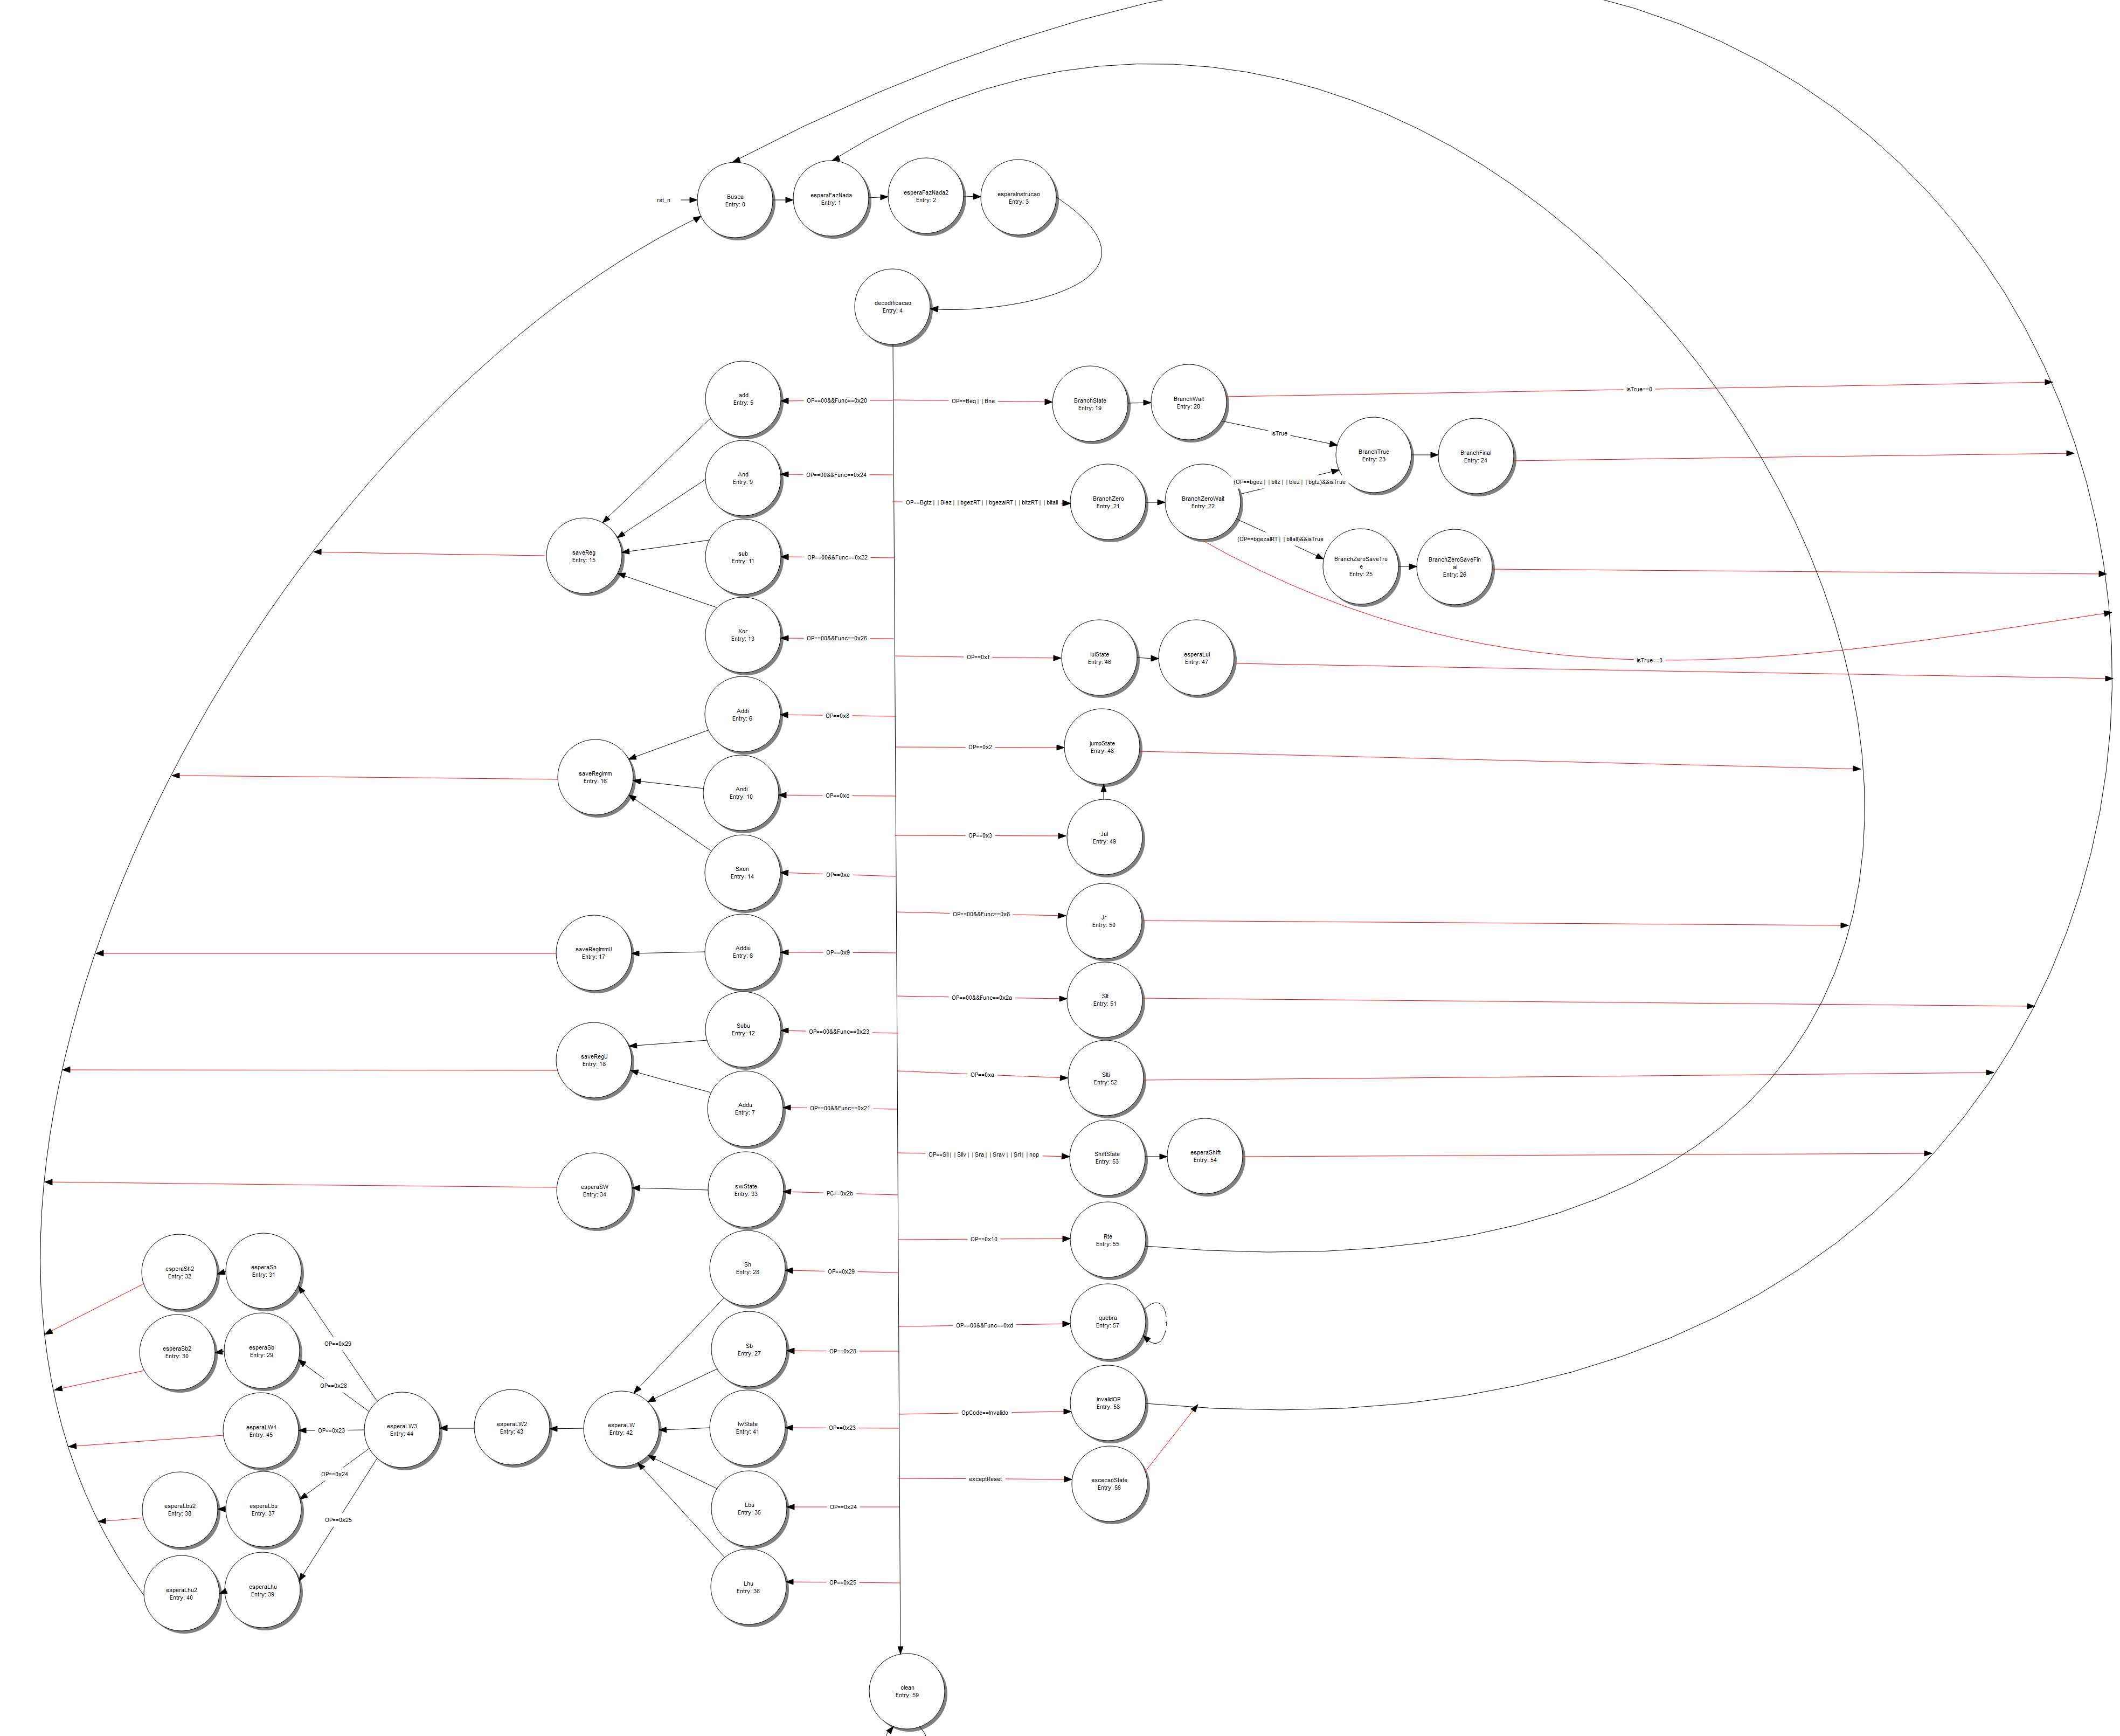
\includegraphics[scale=0.16]{FSM.png}
        \end{center}
    
    \newpage
    \subsection{busca, esperaFazNada, esperaFazNada2, esperaInstrucao}
    Nestes estados, o PC é incrementado em 4 e a instrução é lida da memória e escrita no banco de registradores.
    
    \subsection{decodificacao}
    Neste estado é feita a decodificação da instrução, guiando o estado para a operação a ser executada.
    
    \subsection{add}
    Neste estado é feita a operação de soma entre os registradores rs e rt e a {\it flag} de {\it Overflow} é considerada.
    
    \subsection{And}
    Neste estado é feita a operação de and entre os registradores rs e rt.
    
    \subsection{sub}
    Neste estado é feita a operação de subtração entre os registradores rs e rt e a {\it flag} de {\it Overflow} é considerada.
    
    \subsection{Xor}
    Neste estado é feita a operação de xor entre os registradores rs e rt.
    
    \subsection{Addi}
    Neste estado é feita a operação de soma entre o registrador rs e o imediato e a {\it flag} de {\it Overflow} é considerada.
    
    \subsection{Andi}
    Neste estado é feita a operação de and entre o registrador rs e o imediato.
    
    \subsection{Sxori}
    Neste estado é feita a operação de xor entre o registrador rs e o imediato.
    
    \subsection{Addiu}
    Neste estado é feita a operação de soma entre o registrador rs e o imediato e a {\it flag} de {\it Overflow} não é considerada.
    
    \subsection{Subu}
    Neste estado é feita a operação de subtração entre os registradores rs e rt e a {\it flag} de {\it Overflow} não é considerada.
    
    \subsection{Addu}
    Neste estado é feita a operação de soma entre os registradores rs e rt e a {\it flag} de {\it Overflow} não é considerada.
    
    \subsection{saveReg}
    Neste estado é escrito no registrador rd o valor que sai do registrador aluOut e a {\it flag} de {\it Overflow} é considerada.
    
    \subsection{saveRegImm}
    Neste estado é escrito no registrador rt o valor que sai do registrador aluOut e a {\it flag} de {\it Overflow} é considerada.
    
    \subsection{saveRegImmU}
    Neste estado é escrito no registrador rt o valor que sai do registrador aluOut e a {\it flag} de {\it Overflow} não é considerada.
    
    \subsection{saveRegU}
    Neste estado é escrito no registrador rd o valor que sai do registrador aluOut e a {\it flag} de {\it Overflow} não é considerada.
    
    \subsection{swState}
    Neste estado é calculado o endereço que será armazenado o valor do registrador rt.
    
    \subsection{esperaSw}
    Neste estado é escrito no endereço calculado anteriormente o valor do registrador rt.
    
    \subsection{sh}
    Neste estado é calculado o endereço que será armazenado a {\it half word} menos significativa do registrador rt e o valor de rt é mantido no registrador regB.
    
    \subsection{esperaSh, esperaSh2}
    Nestes estados são combinados o dado lido da memória com a {\it half word} menos significativa do registrador rt e escrito no endereço da memória calculado anteriormente em sh. O estado {\it esperaSh} serve para que o valor lido da memória passe do registrador MDR.
    
    \subsection{sb}
    Neste estado é calculado o endereço que será armazenado o byte menos significativa do registrador rt e o valor de rt é mantido no registrador regB.
    
    \subsection{esperaSb, esperaSb2}
    Nestes estados são combinados o dado lido da memória com o byte menos significativo do registrador rt e escrito no endereço da memória calculado anteriormente em sb. O estado {\it esperaSb} serve para que o valor lido da memória passe do registrador MDR.
    
    \subsection{lwState, esperaLW, esperaLW2, esperaLW3}
    Nestes estados é calculado o endereço que será lido da memória e é esperado o tempo necessário para que o dado lido da memória chegue no banco de memória e passe do registrador MDR.
    
    \subsection{esperaLW4}
    Neste estado é escrito o dado lido da memória no registrador rt.
    
    \subsection{Lbu}
    Neste estado é calculado o endereço que será lido da memória e escrito no byte menos significativo do registrador.
    
    \subsection{esperaLbu, esperaLbu2}
    Nestes estados é escrito a combinação do byte menos significativo lido da memória com 0s no registrador rt. O estado {\it esperaLbu} serve para que o valor lido da memória passe do registrador MDR.
    
    \subsection{Lhu}
    Neste estado é calculado o endereço que será lido da memória e escrito na {\it half word} menos significativa do registrador.
    
    \subsection{esperaLhu, esperaLhu2}
    Nestes estados é escrito a combinação da {\it half word} menos significativa lido da memória com 0s no registrador rt. O estado {\it esperaLhu} serve para que o valor lido da memória passe do registrador MDR.
    
    \subsection{BranchState, BranchWait}
    Nestes estados são analisados os registradores rs e rt para saber se o desvio será feito ou não. O estado {\it BranchWait} serve para dar tempo para que o módulo branchSelector forneça o dado certo.
    
    \subsection{BranchZero, BranchZeroWait}
    Nestes estados é analisado o registrador rs em relação ao valor 0 para saber se o desvio será feito ou não. O estado {\it BranchWait} serve para dar tempo para que o módulo branchSelector forneça o dado certo.
    
    \subsection{BranchTrue, BranchFinal}
    Nestes estados, o desvio é calculado e escrito em PC.
    
    \subsection{BranchZeroSaveTrue, BranchZeroSaveFinal}
    Nestes estados, o valor atual de PC é salvo no registrador 31 e o desvio é calculado e escrito em PC.
    
    \subsection{luiState, esperaLui}
    Nestes estados, o valor imediato da operação é estendido para 32 bits (preenchendo os 16 bits mais significativos com o valor do imediato) e, no estado {\it esperaLui}, o valor é escrito no registrador rt.
    
    \subsection{jumpState}
    Neste estado, é calculado o valor do jump e este valor é escrito em PC.
    
    \subsection{Jal}
    Neste estado, o valor de PC é escrito no registrador 31.
    
    \subsection{Jr}
    Neste estado, o valor de rs é escrito em PC.
    
    \subsection{Slt}
    Neste estado, é feito a subtração entre os registradores rs e rt e a {\it flag} negativo é escrita no registrador rd.
    
    \subsection{Slti}
    Neste estado, é feito a subtração entre os registradores rs e imediato e a {\it flag} negativo é escrita no registrador rt.
    
    \subsection{ShiftState}
    Nestes estados, é feita a operação de sll, sllv, nop, sra, srav ou slr.
    
    \subsection{esperaShift}
    Neste estado é escrito o dado que saiu do registrador de deslocamento no registrador rd.
    
    \subsection{Rte}
    Neste estado é escrito o valor que sai do registrador EPC em PC.
    
    \subsection{quebra}
    Este estado é um loop infinito que faz com que o processador pare a execução.
    
    \subsection{excecaoState}
    Este estado é ativado quando a {\it flag} de {\it Overflow} é ativada.
    
    \subsection{invalidOP}
    Neste estado é salvo o endereço de PC da instrução que teve um {\it OP Code} inválido.
    
    \subsection{clean}
    Neste estado, todo o sistema é reiniciado: todos os registradores são zerados.
    
    \newpage
    \begin{center}
        \begin{table}[]
        \centering
        \caption{\textbf{Número dos estados}}
        \label{my-label}
        \begin{tabular}{llll}
        \\
        0: Busca           & 16: saveRegImm          & 32: esperaSh2  & 48: jumpState    \\
        1: esperaFazNada   & 17: saveRegImmU         & 33: swState    & 49: Jal          \\
        2: esperaFazNada2  & 18: saveRegU            & 34: esperaSw   & 50: Jr           \\
        3: esperaInstrucao & 19: BranchState         & 35: Lbu        & 51: Slt          \\
        4: decodificacao   & 20: BranchWait          & 36: Lhu        & 52: Slti         \\
        5: add             & 21: BranchZero          & 37: esperaLbu  & 53: ShiftState   \\
        6: Addi            & 22: BranchZeroWait      & 38: esperaLbu2 & 54: esperaShift  \\
        7: Addu            & 23: BranchTrue          & 39: esperaLhu  & 55: rte          \\
        8: Addiu           & 24: BrachFinal          & 40: esperaLhu2 & 56: excecaoState \\
        9: And             & 25: BranchZeroSaveTrue  & 41: lwState    & 57: quebra       \\
        10: Andi           & 26: BranchZeroSaveFinal & 42: esperaLw   & 58: invalidOP    \\
        11: sub            & 27: Sb                  & 43: esperaLw2  & 59: clean        \\
        12: Subu           & 28: Sh                  & 44: esperaLw3  &                  \\
        13: Xor            & 29: esperaSb            & 45: esperaLw4  &                  \\
        14: Sxori          & 30: esperaSb2           & 46: luiState   &                  \\
        15: saveReg        & 31: esperaSh            & 47: esperaLui  &                  \\               
        \end{tabular}
        \end{table}
    \end{center}
    
    \newpage
    \section{Conjunto de Simulações}
    \subsection{Instruções}
    Todas as operações são simuladas no módulo {\it MultCycleProcessor}\footnote{Descrito na página 7.}. Tem como:\\
    \textbf{Entradas}:
    \begin{enumerate}
        \item clk(1 bit): representa o clock do sistema.
        \item rst(1 bit): representa que, quando ativado, reinicia todo o sistema.\\
    \end{enumerate}
\\
    \textbf{Saídas}:
    \begin{enumerate}
        \item overflowFlag(1 bit): representa se o sinal de Overflow foi ativado.
        \item whoIsA(5 bits): representa qual registrador foi transferido pro RegA.
        \item whoIsB(5 bits): representa qual registrador foi transferido pro RegB.
        \item WriteRegister(5 bits): representa qual registrador vai ser possivelmente escrito.
        \item estado(7 bits): representa o estado no qual a Unidade de Controle se encontra.
        \item MemData(32 bits): representa o dado que está na saída do registrador de acesso a memória.
        \item WriteDataMem(32 bits): representa o dado que será possivelmente escrito na memória.
        \item WriteDataReg(32 bits): representa o dado que será possivelmente escrito em um registrador.
        \item MDR(32 bits): representa o dado que está na saída do registrador Memory Data Register.
        \item Alu(32 bits): representa o dado que está na saída da ULA.
        \item AluOut(32 bits): representa o dado que está na saída do registrador AluOut.
        \item PC(32 bits): representa o dado que está na saída do registrador PC (Program Counter).
        \item Address(32 bits): representa o endereço que vai ser lido/escrito na memória.
        \item instrucao(32 bits): representa a instrução que está saindo do Registrador de Instruções.
        \item EPC\_out(32 bits): representa o dado que está na saída do registrador EPC (Excepcion Program Counter).\\
    \end{enumerate}\\
    Ao olhar a imagem, analisar os dados que estão à direita do {\it pivot} do {\it waveform} do {\it Quartus}.\\
    Código usado para observar o funcionamento do: lui, jal, break, add, addi, addiu, addu, sub, subu, and, andi, xor, xori, beq(falha), bne(falha), sw, lw, slt, slti, nop, sll, sllv, sra, srav, srl e jr:
    \begin{verbatim}
        lui $2, 1
        jal 4
        lui $4, 1
        break
        add $5, $2, $0
        addi $6, $2, 1
        addiu $7, $0, 1
        addu $8, $6, $0
        sub $9, $6, $6
        subu $9, $7, $2
        and $10, $7, $2
        andi $6, $5, 1
        xor $11, $2, $0
        xori $12, $2, 2
        beq $12, $11, 0
        bne $12, $12, 0
        sw $2, 180($0)
        lw $13, 180($0)
        slt $14, $2, $3
        slt $14, $0, $2
        slti $14, $0, 0
        slti $14, $0, 2
        nop
        lui $2, 1
        addi $5, $0, 4
        sll $4, $2, 3
        sllv $4, $2, $5
        sra $4, $2, 3
        srav $4, $2, $5
        srl $4, $2, 3
        jr $31
        break
    \end{verbatim}
    \\
    Código usado para testar os branchs:\\
    \begin{verbatim}
        addi $2, $0, -1
        addi $3, $0, 1
        bgez $2, 12
        bgezal $2, 14
        bgtz $0, 14
        blez $3, 5
        bltz $0, 8
        bltall $0, 5
        nop
        bgez $0, 1
        break
        bgezal $3, 1
        break
        bgtz $3, 1
        break
        blez $0, 1
        break
        bltz $2, 1
        break
        bltall $2, 1
        break
        beq $2, $2, 1
        break
        bne $2, $3, 1
        break
        nop
        nop
        break
    \end{verbatim}
    \\
    Código usado para testar o lbu, lhu, sb e sh:\\
    \begin{verbatim}
        addi $2, $0, 256
        addi $3, $0, 1
        addi $4, $0, 32768
        addi $4, $4, 32768
        sw $4, 100($0)
        sw $4, 110($0)
        sb $2, 100($0)
        sh $2, 110($0)
        lb $5, 100($0)
        lh $5, 110($0)
        sb $3, 100($0)
        sh $3, 110($0)
        lh $5, 100($0)
        lb $5, 110($0)
        break
    \end{verbatim}
    \\
    Código usado para testar o j e o rte:\\
    \begin{verbatim}
        nop
        j 6
        nop
        nop
        nop
        nop
        rte
        break
    \end{verbatim}
    \newpage
    \subsubsection{add}
    {\it add \$5, \$2, \$0}\\
    \begin{center}
        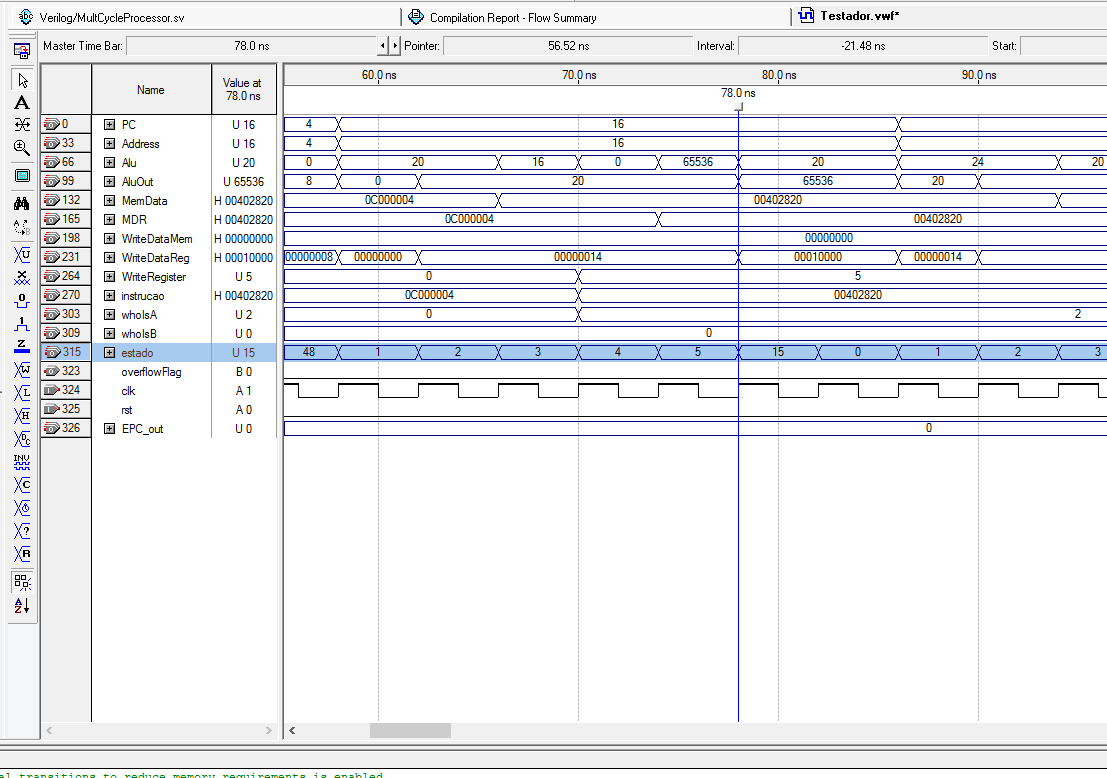
\includegraphics[scale=0.25]{add.PNG}
    \end{center}
    
    \\
    \subsubsection{addu}
    {\it addu \$8, \$6, \$0}\\
    \begin{center}
        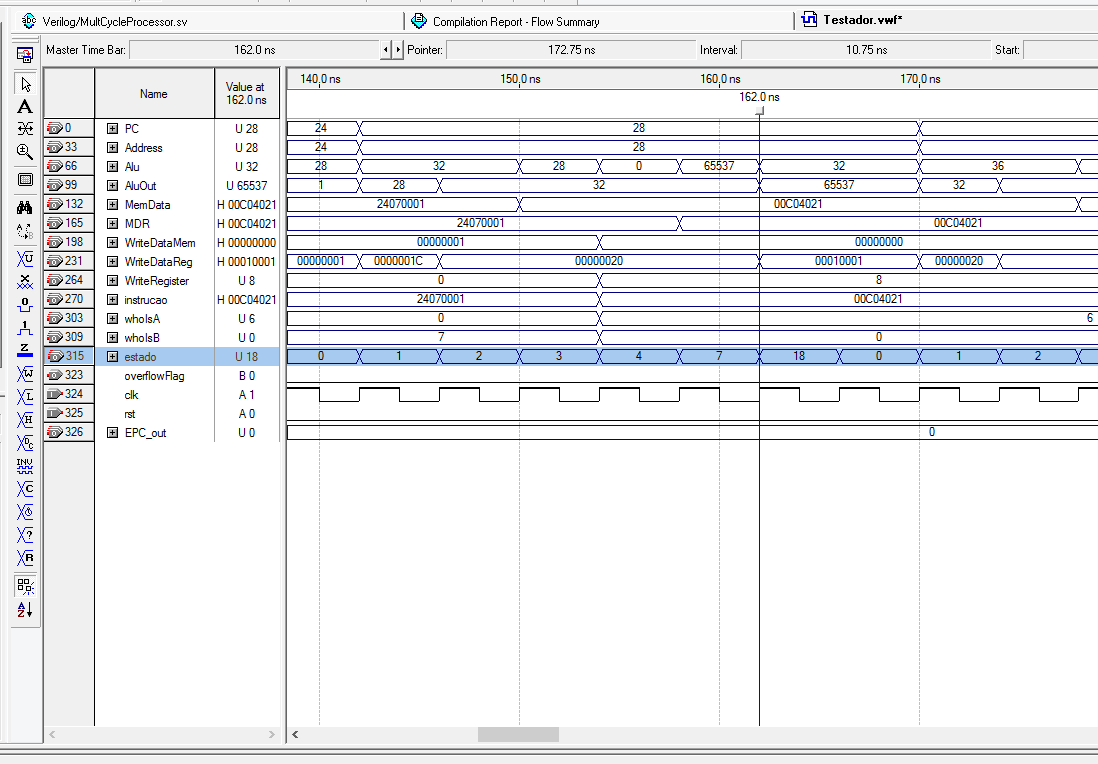
\includegraphics[scale=0.25]{addu.PNG}
    \end{center}
    
    \\
    \subsubsection{and}
    {\it and \$10, \$7, \$2}\\
    \begin{center}
        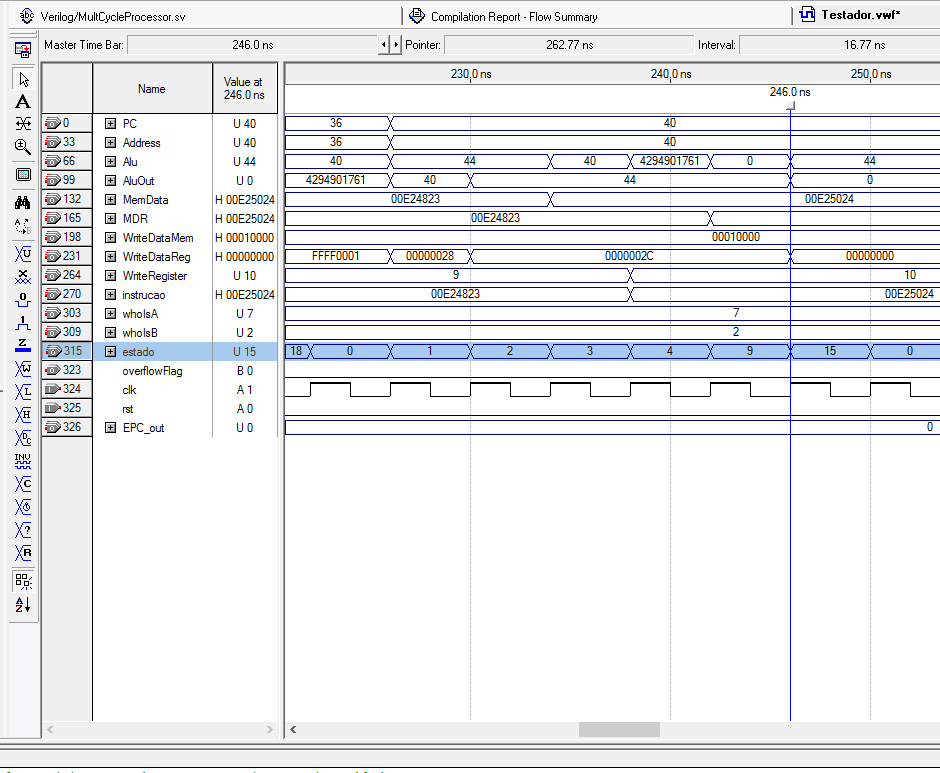
\includegraphics[scale=0.25]{and.PNG}
    \end{center}
    
    \\
    \subsubsection{jr}
    {\it jr \$31}\\
    \begin{center}
        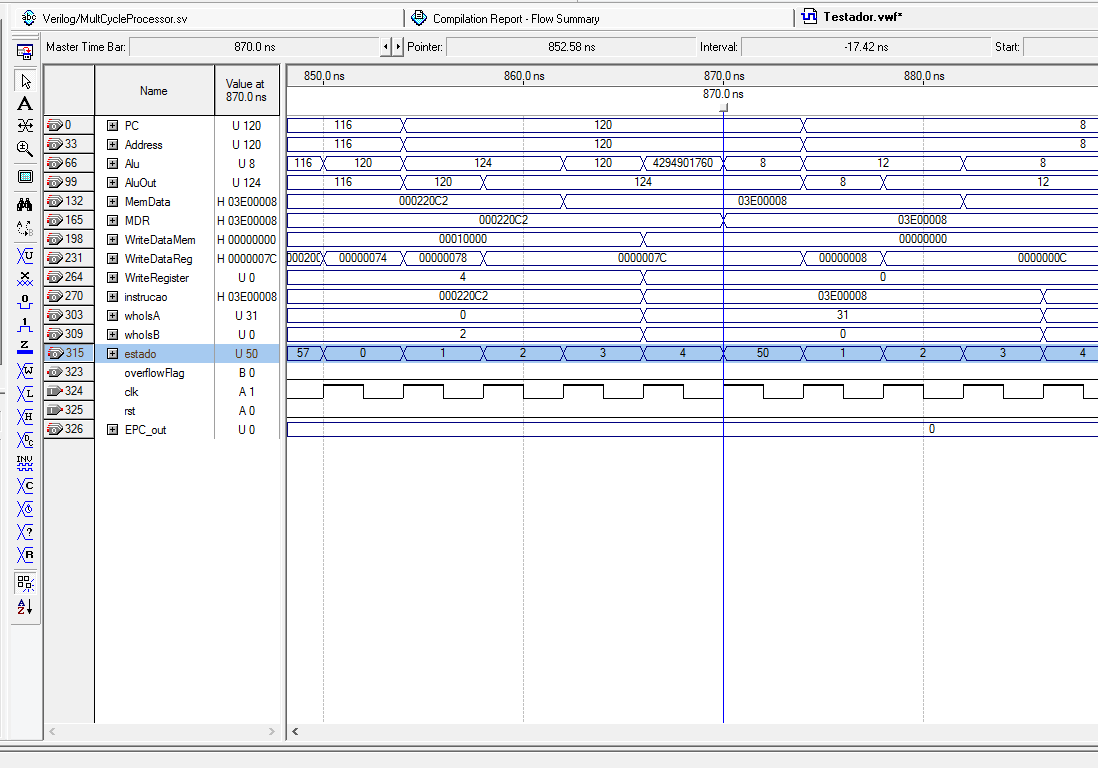
\includegraphics[scale=0.25]{jr.PNG}
    \end{center}
    
    \\    
    \subsubsection{sll e nop}
    {\it nop}\\
    \begin{center}
        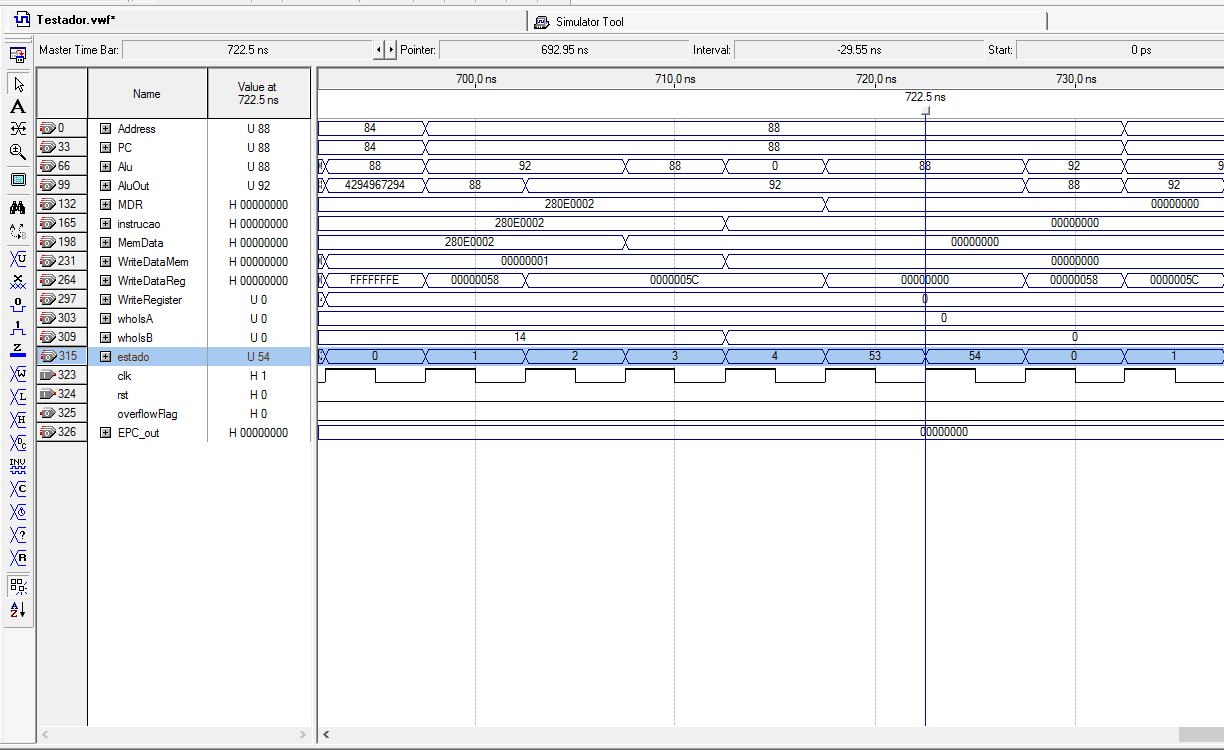
\includegraphics[scale=0.25]{nop.PNG}
    \end{center}
    \\
    {\it sll \$4, \$2, 3}\\
    \begin{center}
        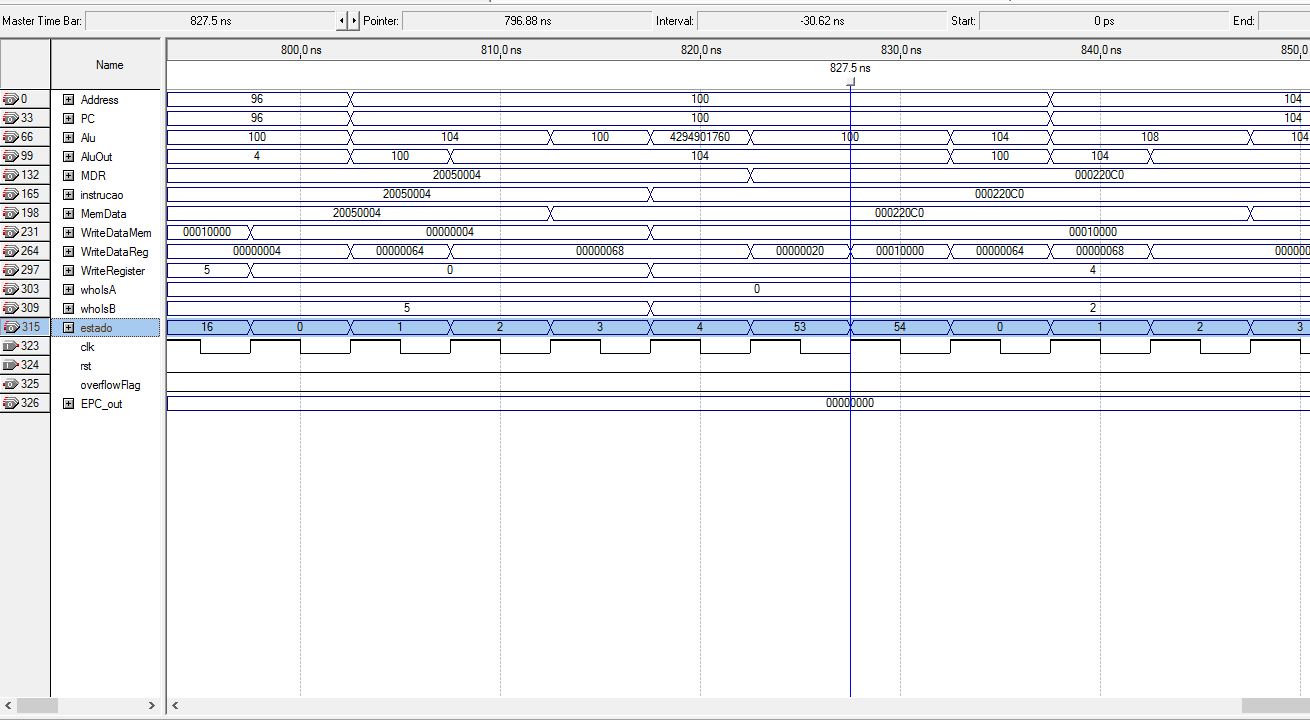
\includegraphics[scale=0.25]{sll.PNG}
    \end{center}
    
    \newpage
    \subsubsection{sllv}
    {\it sllv \$4, \$2, \$5}\\
    \begin{center}
        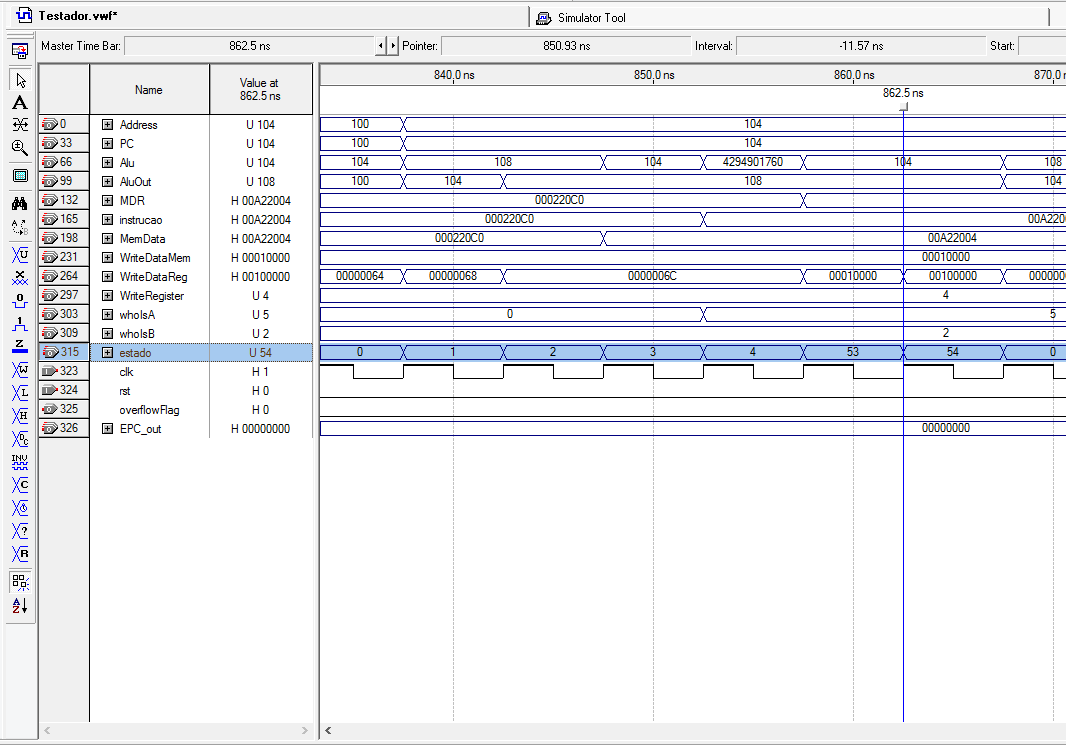
\includegraphics[scale=0.25]{sllv.PNG}
    \end{center}
    
    \\    
    \subsubsection{sra}
    {\it sra \$4, \$2, 3}\\
    \begin{center}
        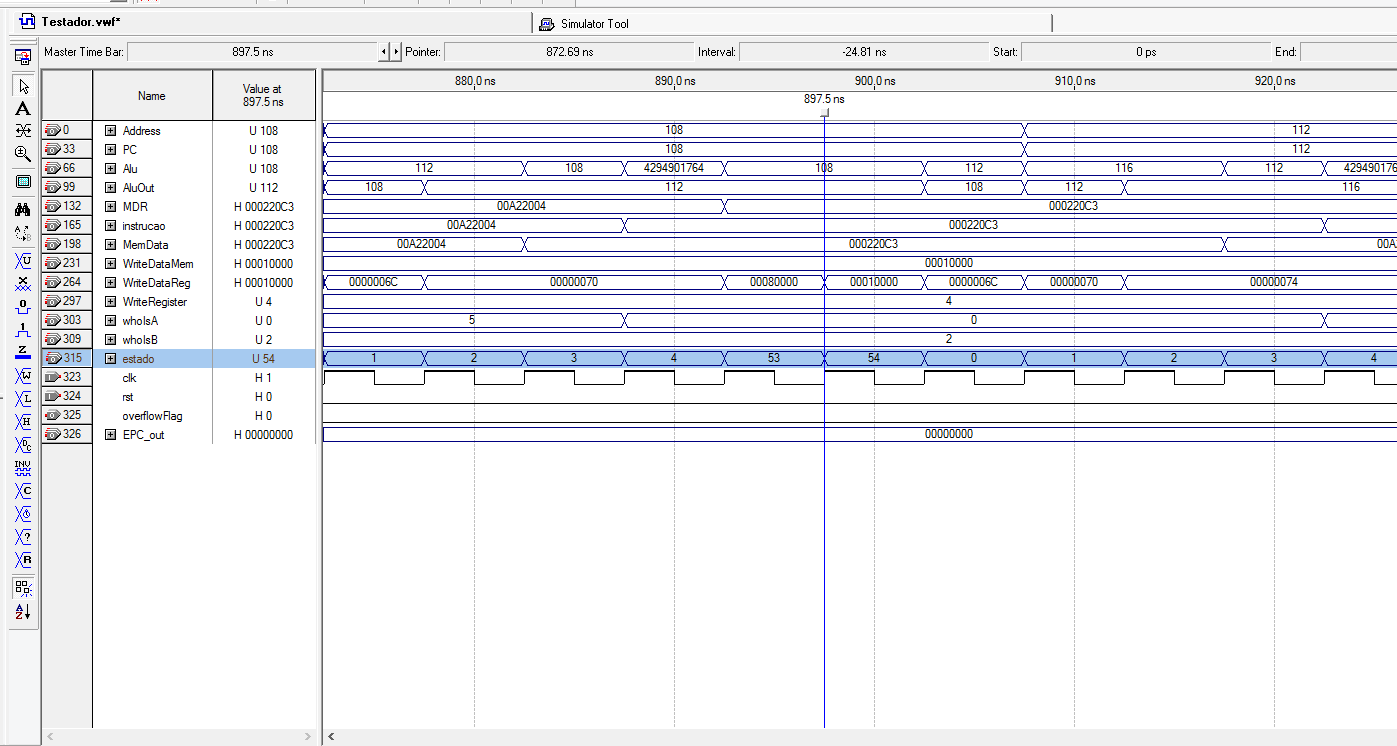
\includegraphics[scale=0.25]{sra.PNG}
    \end{center}
    
    \\    
    \subsubsection{srav}
    {\it srav \$4, \$2, \$5}\\
    \begin{center}
        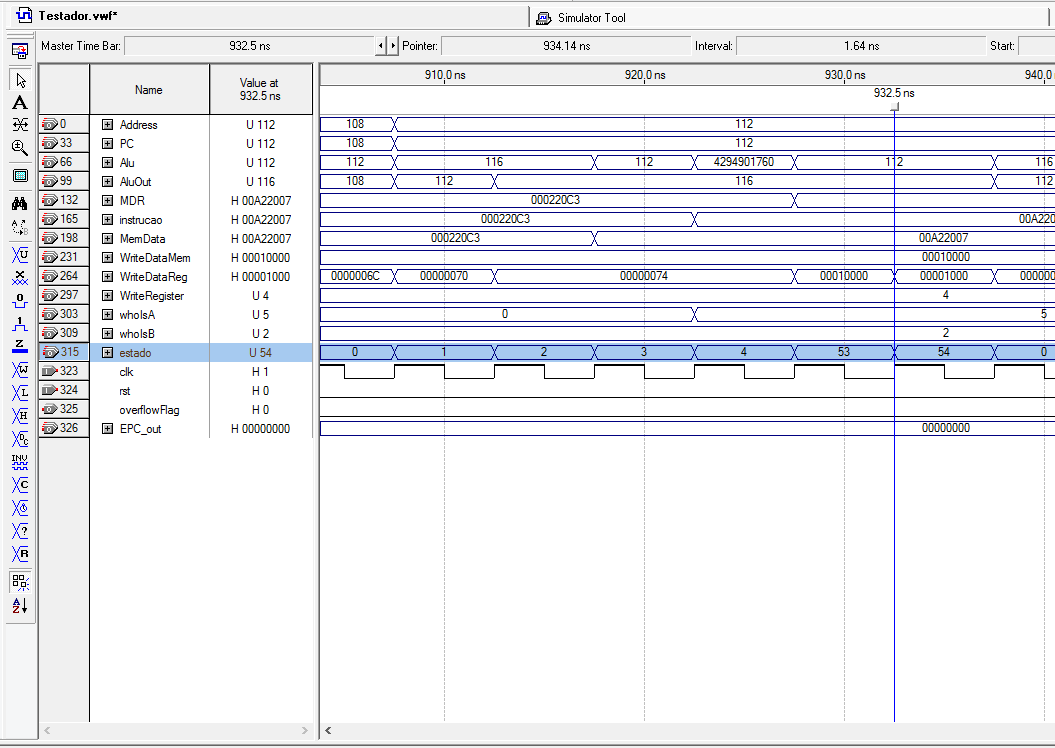
\includegraphics[scale=0.25]{srav.PNG}
    \end{center}
    
    \\    
    \subsubsection{srl}
    {\it srl \$4, \$2, 3}\\
    \begin{center}
        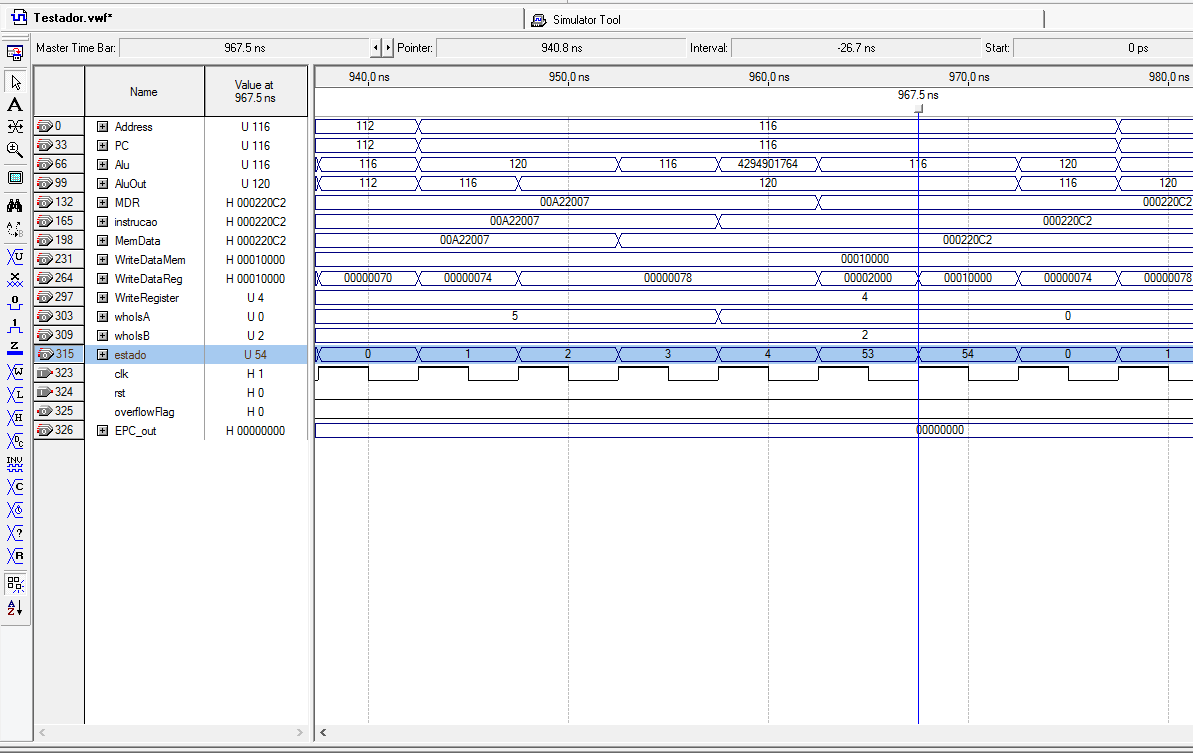
\includegraphics[scale=0.25]{srl.PNG}
    \end{center}
    
    
    \\    
    \subsubsection{slt}
    {\it slt \$14, \$2, \$3} falha;\\
    \begin{center}
        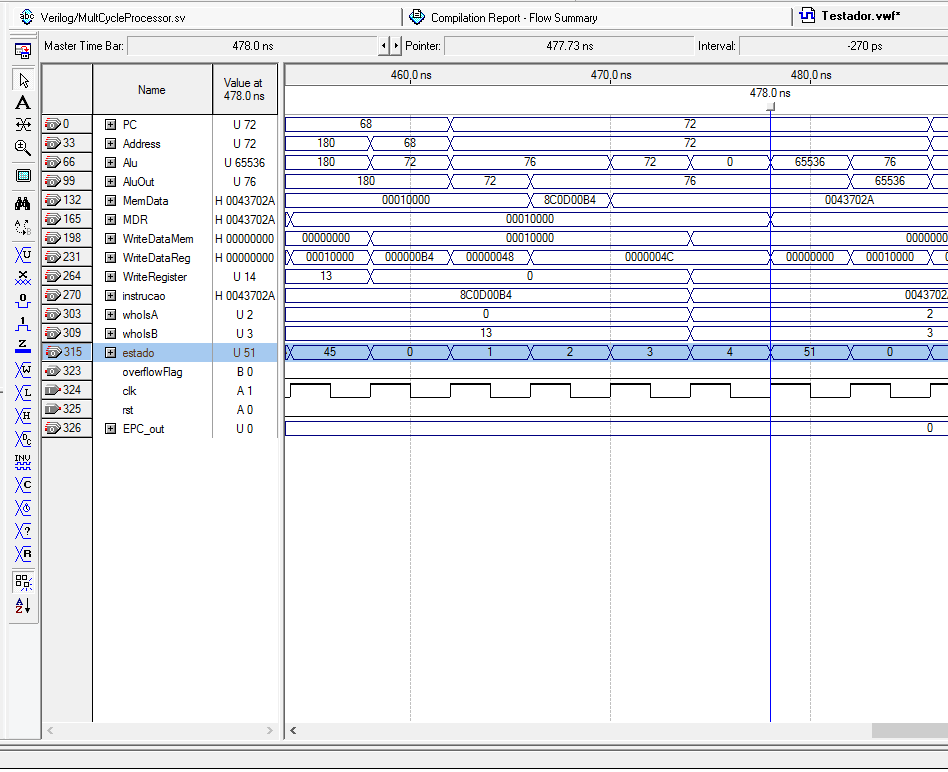
\includegraphics[scale=0.25]{sltfalha.PNG}
    \end{center}
    \\
    {\it slt \$14, \$0, \$2} sucesso;\\
    \begin{center}
        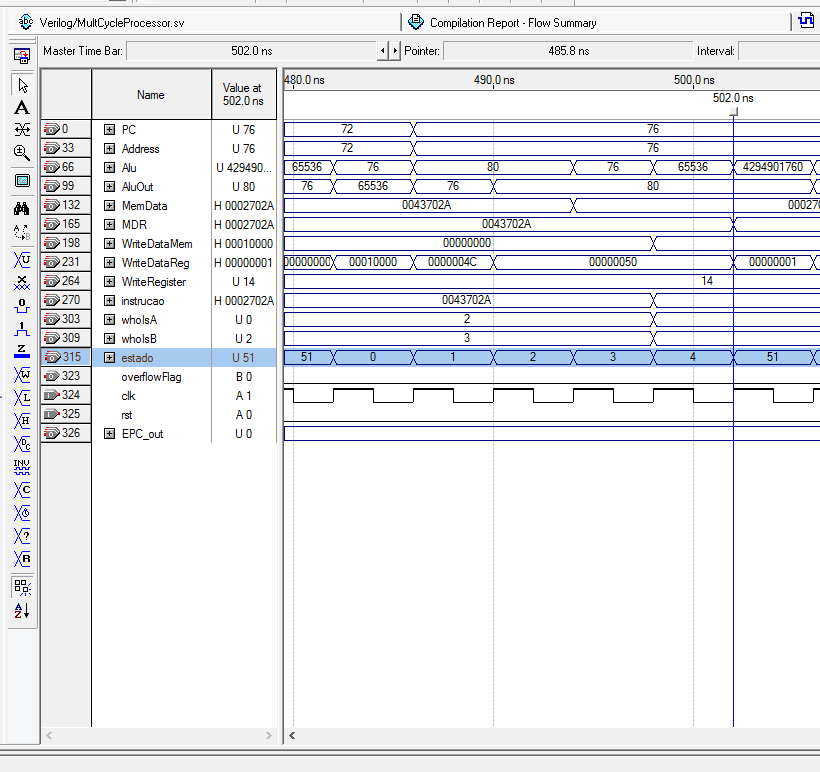
\includegraphics[scale=0.25]{sltsucesso.PNG}
    \end{center}
    
    \\
    \subsubsection{sub}
    {\it sub \$9, \$6, \$6}\\
    \begin{center}
        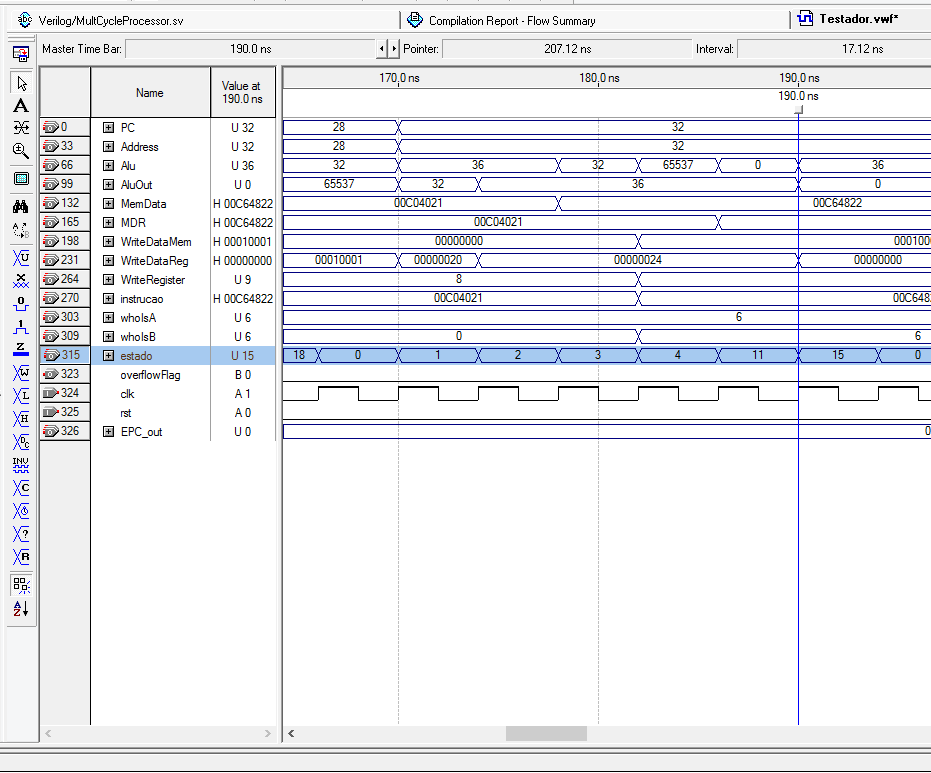
\includegraphics[scale=0.25]{sub.PNG}
    \end{center}
    
    \\
    \subsubsection{subu}
    {\it subu \$9, \$7, \$2}\\
    \begin{center}
        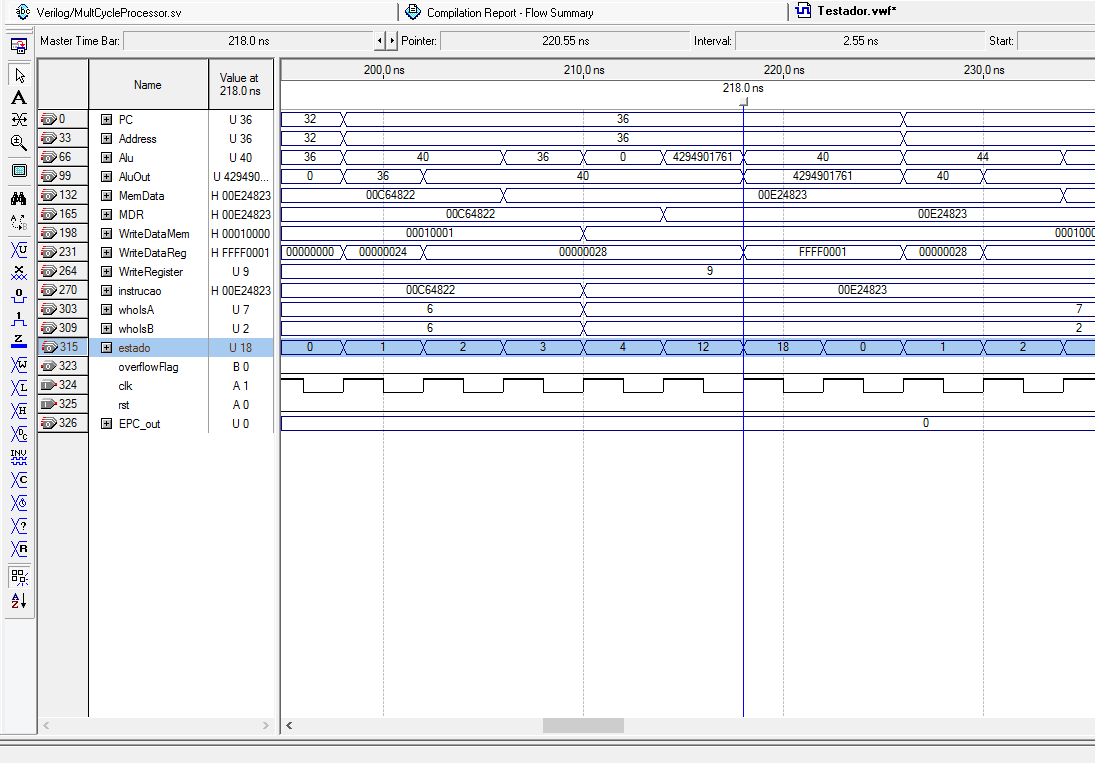
\includegraphics[scale=0.25]{subu.PNG}
    \end{center}
    
    \\
    \subsubsection{xor}
    {\it xor \$11, \$2, \$0}\\
    \begin{center}
        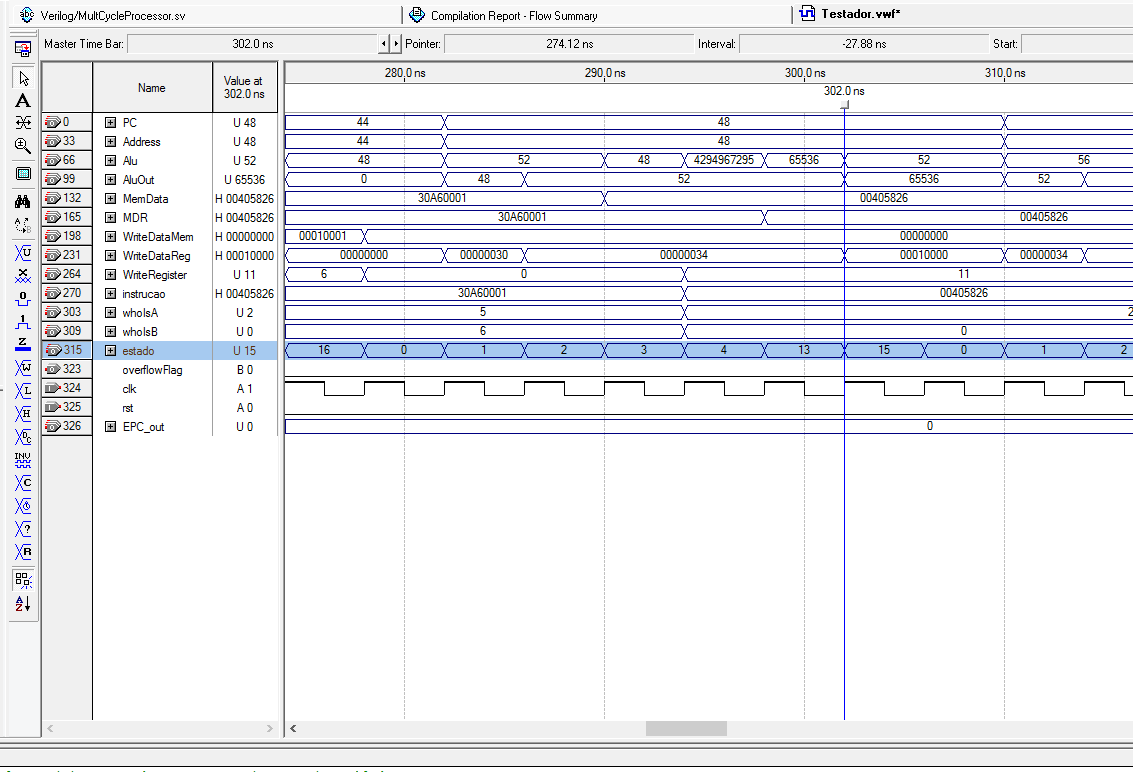
\includegraphics[scale=0.25]{xor.PNG}
    \end{center}
    
    \\
    \subsubsection{break}
    {\it break}\\
    \begin{center}
        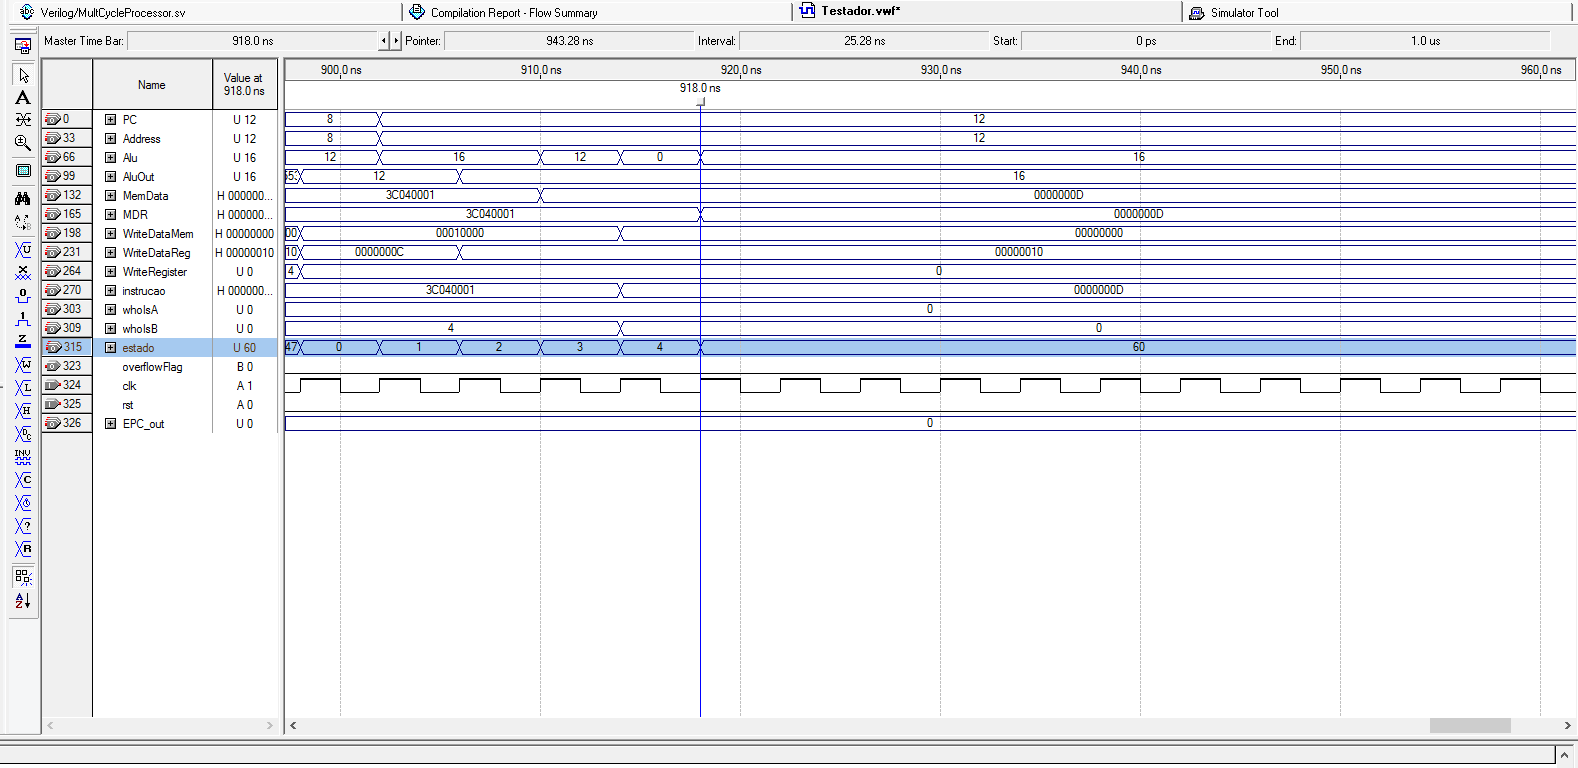
\includegraphics[scale=0.25]{break.PNG}
    \end{center}
    
    \\
    \subsubsection{addi}
    {\it addi \$6, \$2, 1}\\
    \begin{center}
        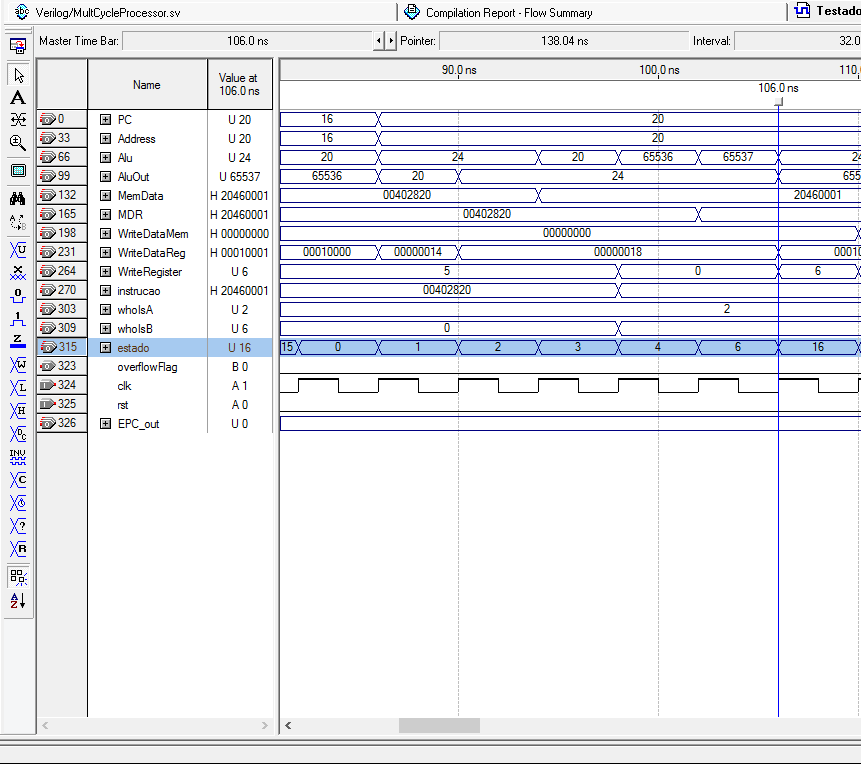
\includegraphics[scale=0.25]{addi.PNG}
    \end{center}
    
    \\
    \subsubsection{addiu}
    {\it addiu \$7, \$0, 1}\\
    \begin{center}
        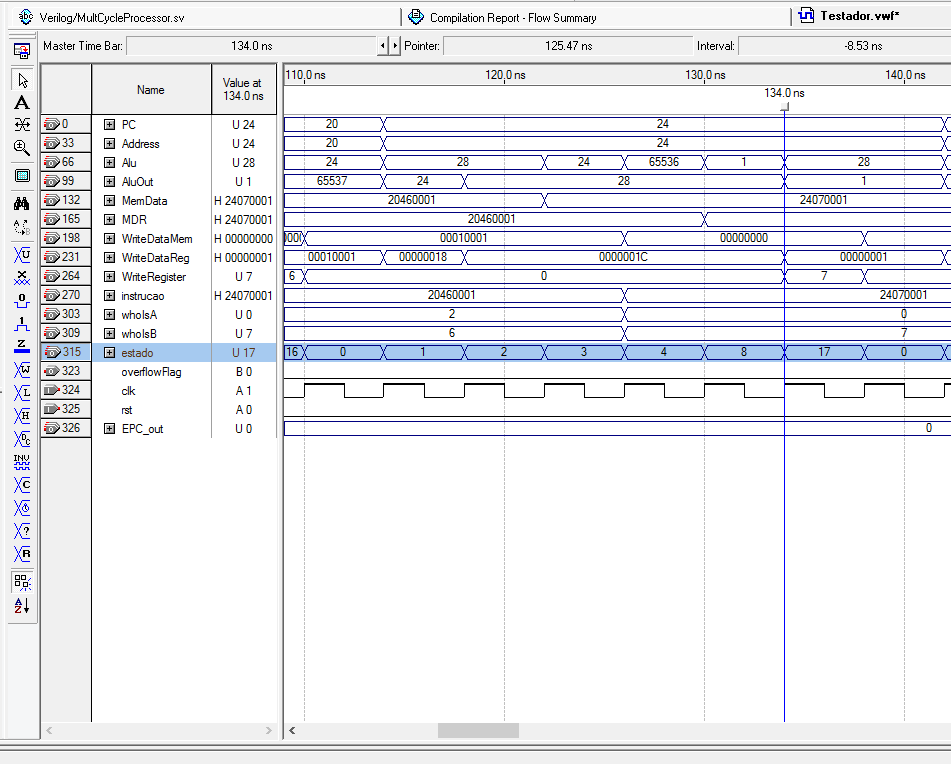
\includegraphics[scale=0.25]{addiu.PNG}
    \end{center}
    
    \\
    \subsubsection{andi}
    {\it andi \$6, \$5, 1}\\
    \begin{center}
        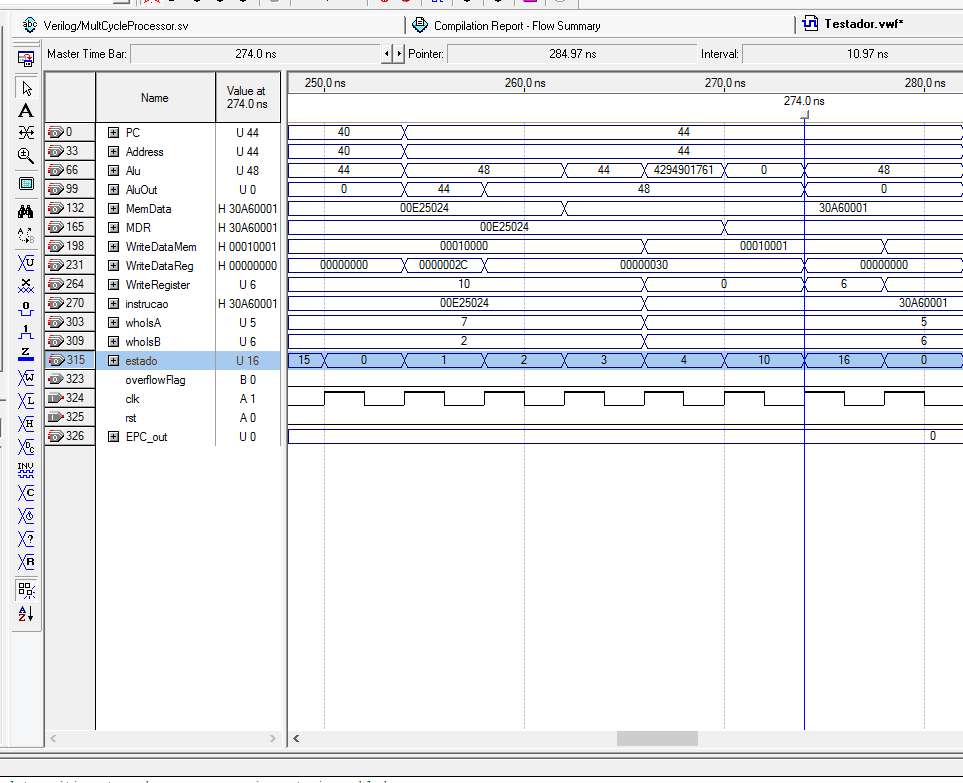
\includegraphics[scale=0.25]{andi.PNG}
    \end{center}
    
    \\
    \subsubsection{beq}
    {\it beq \$12, \$11, 0} falha;\\
    \begin{center}
        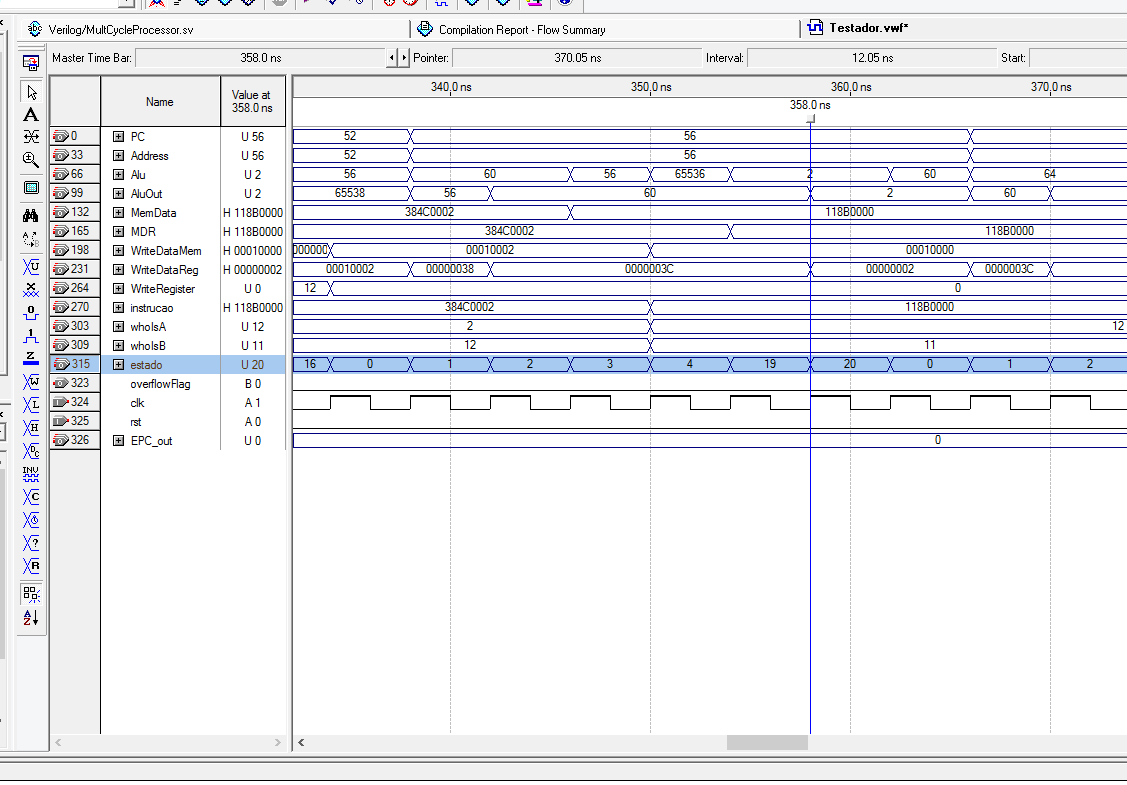
\includegraphics[scale=0.25]{beqfalha.PNG}
    \end{center}
    \\
    {\it beq \$2, \$2, 1} sucesso;\\
    \begin{center}
        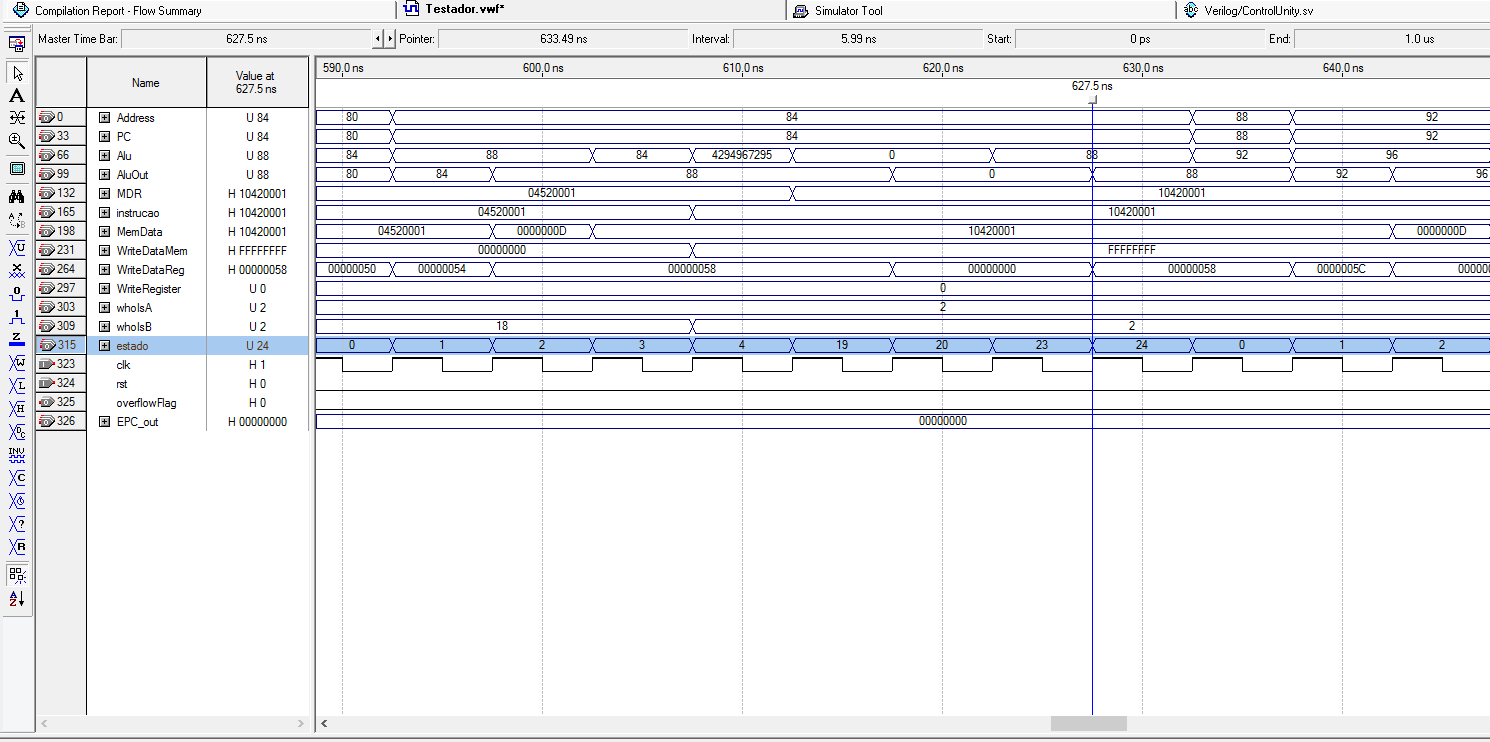
\includegraphics[scale=0.25]{beqsucesso.PNG}
    \end{center}
    
    \\
    \subsubsection{bne}
    {\it bne \$12, \$12, 0} falha;\\
    \begin{center}
        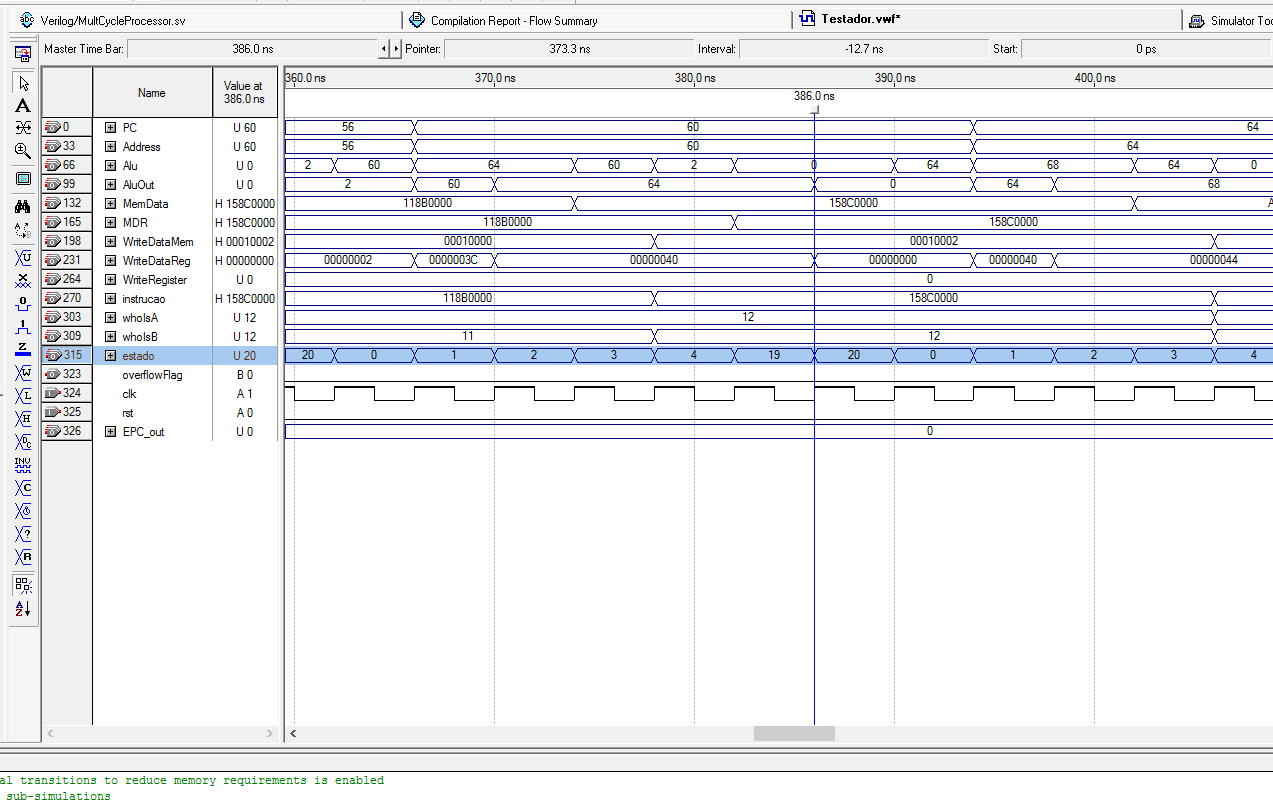
\includegraphics[scale=0.25]{bnefalha.PNG}
    \end{center}
    \\
    {\it bne \$2, \$3, 1} sucesso;\\
    \begin{center}
        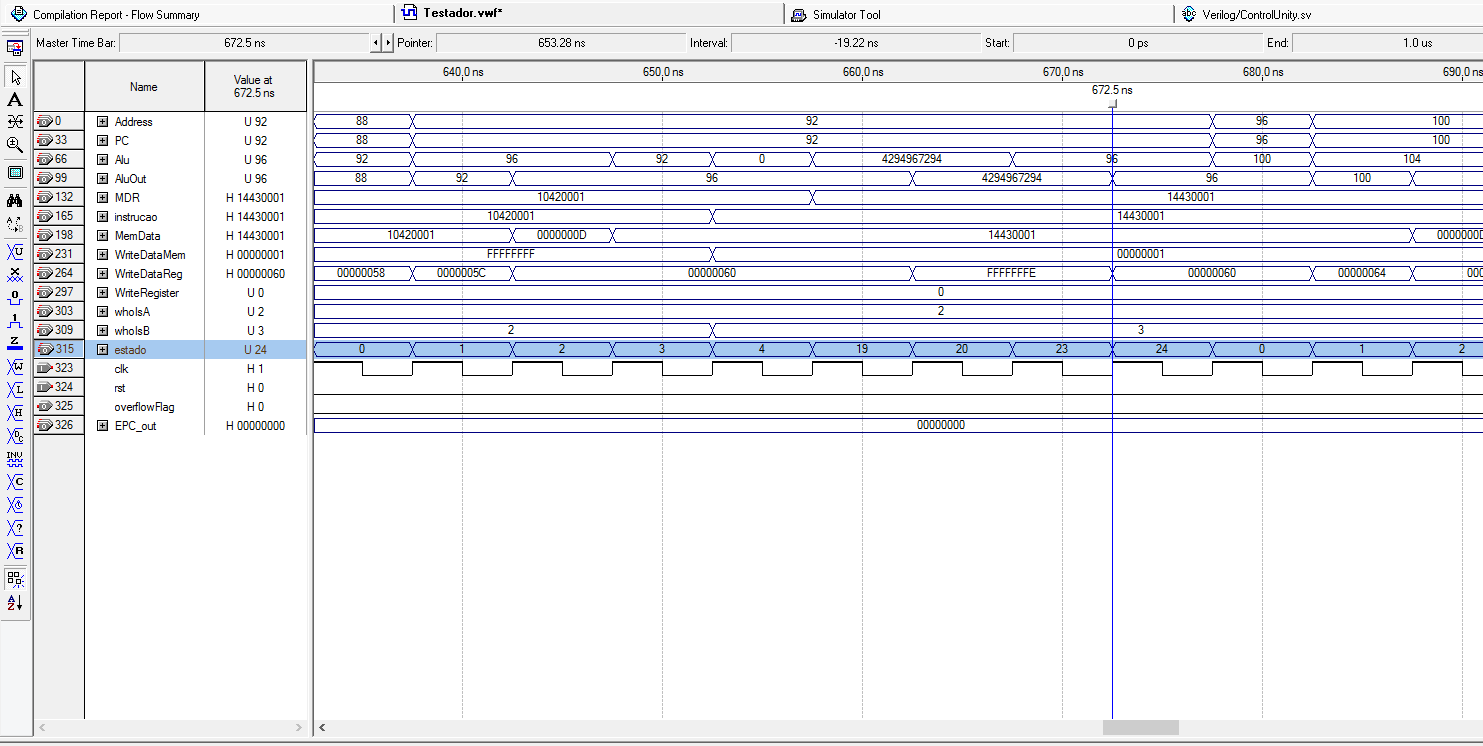
\includegraphics[scale=0.25]{bnesucesso.PNG}
    \end{center}
    
    \\
    \subsubsection{bgez}
    {\it bgez \$2, 0} falha;\\
    \begin{center}
        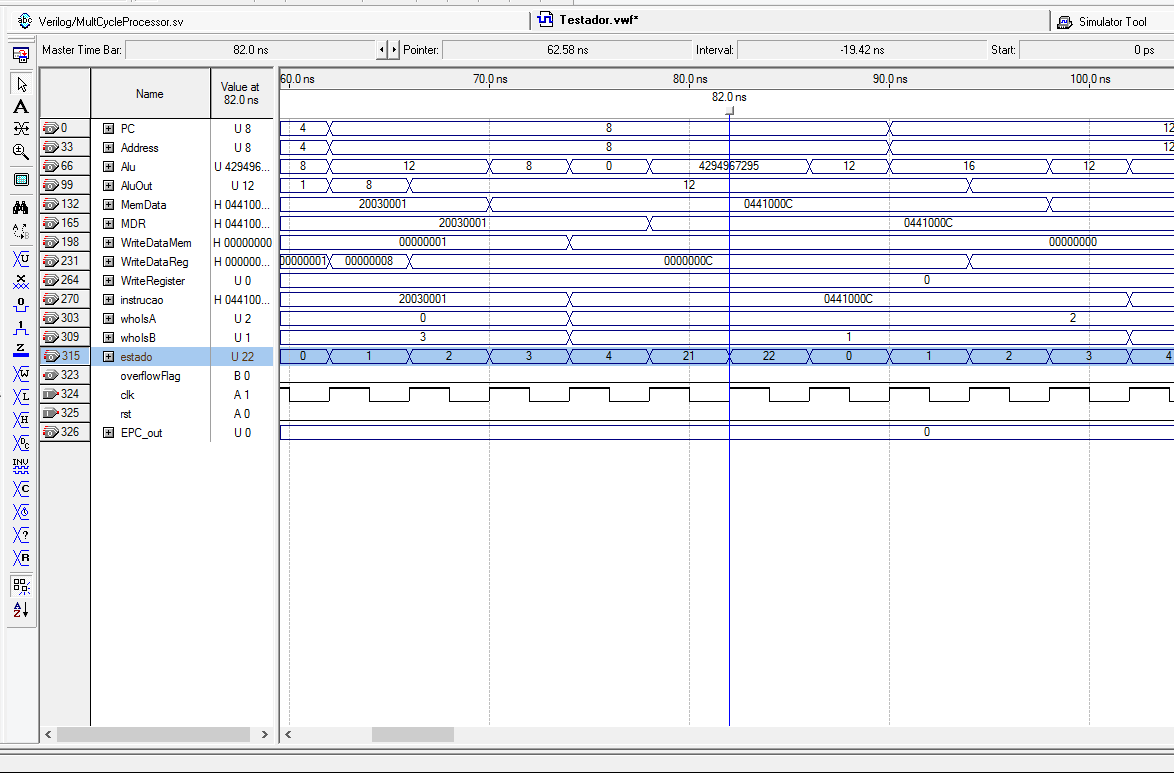
\includegraphics[scale=0.25]{bgezfalha.PNG}
    \end{center}
    \\
    \newpage
    {\it bgez \$0, 1} sucesso;\\
    \begin{center}
        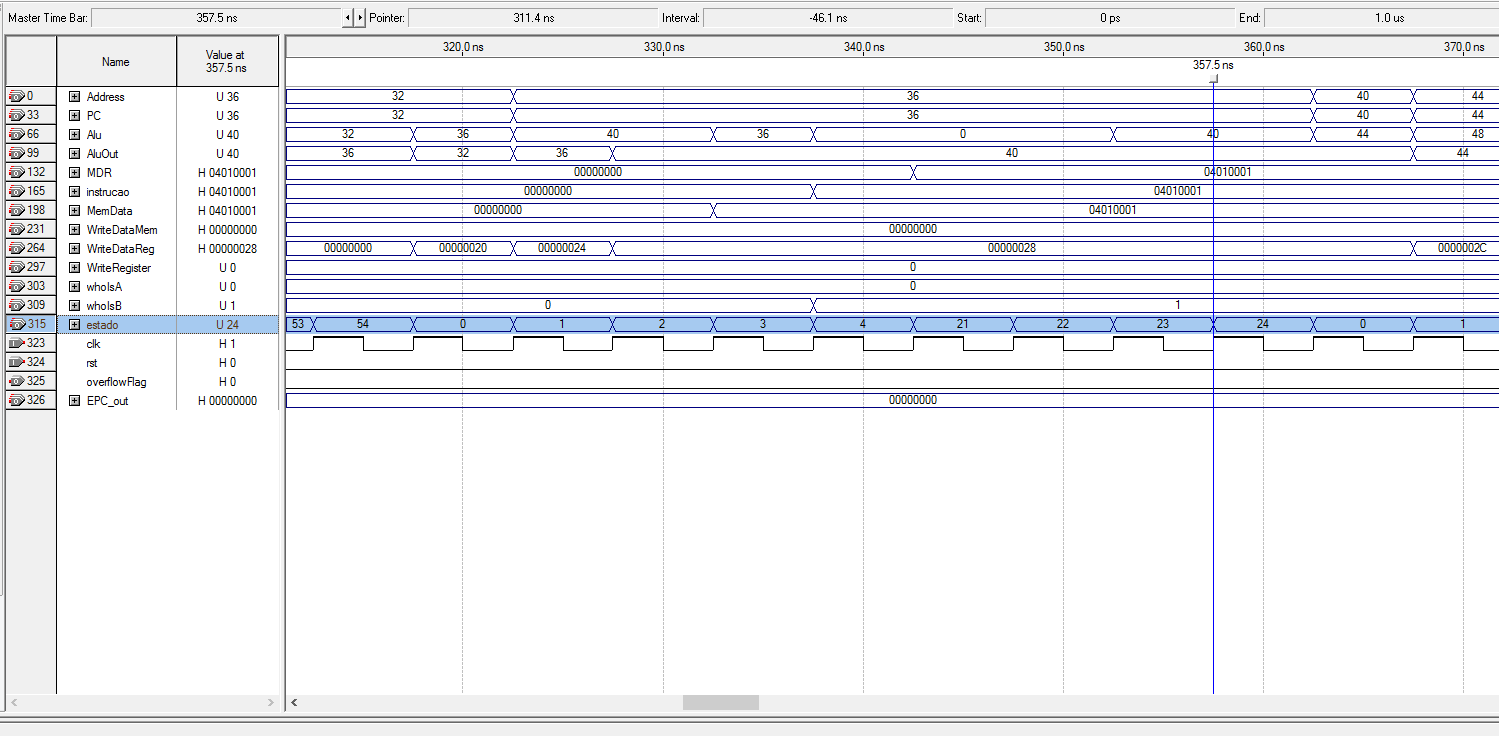
\includegraphics[scale=0.25]{bgezsucesso.PNG}
    \end{center}
    
    \\
    \subsubsection{bgtz}
    {\it bgtz \$0, 14} falha;\\
    \begin{center}
        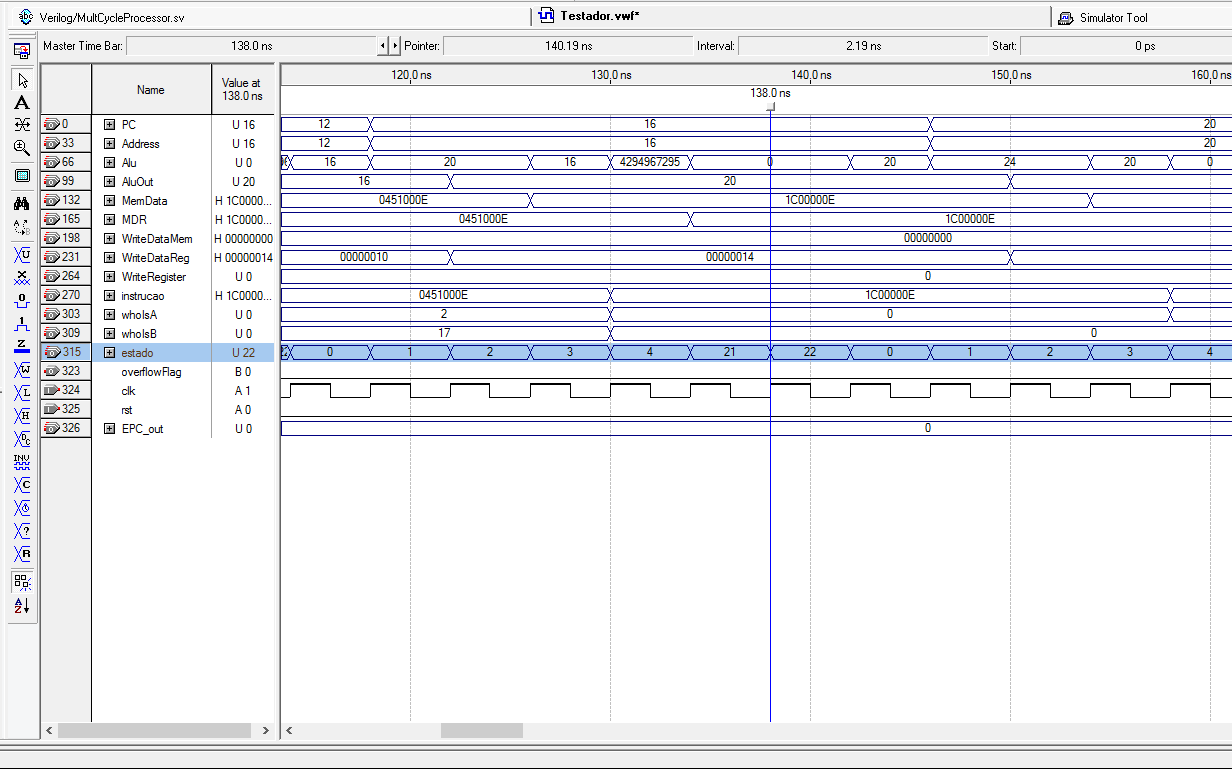
\includegraphics[scale=0.25]{bgtzfalha.PNG}
    \end{center}
    \\
    {\it bgtz \$3, 1} sucesso;\\
    \begin{center}
        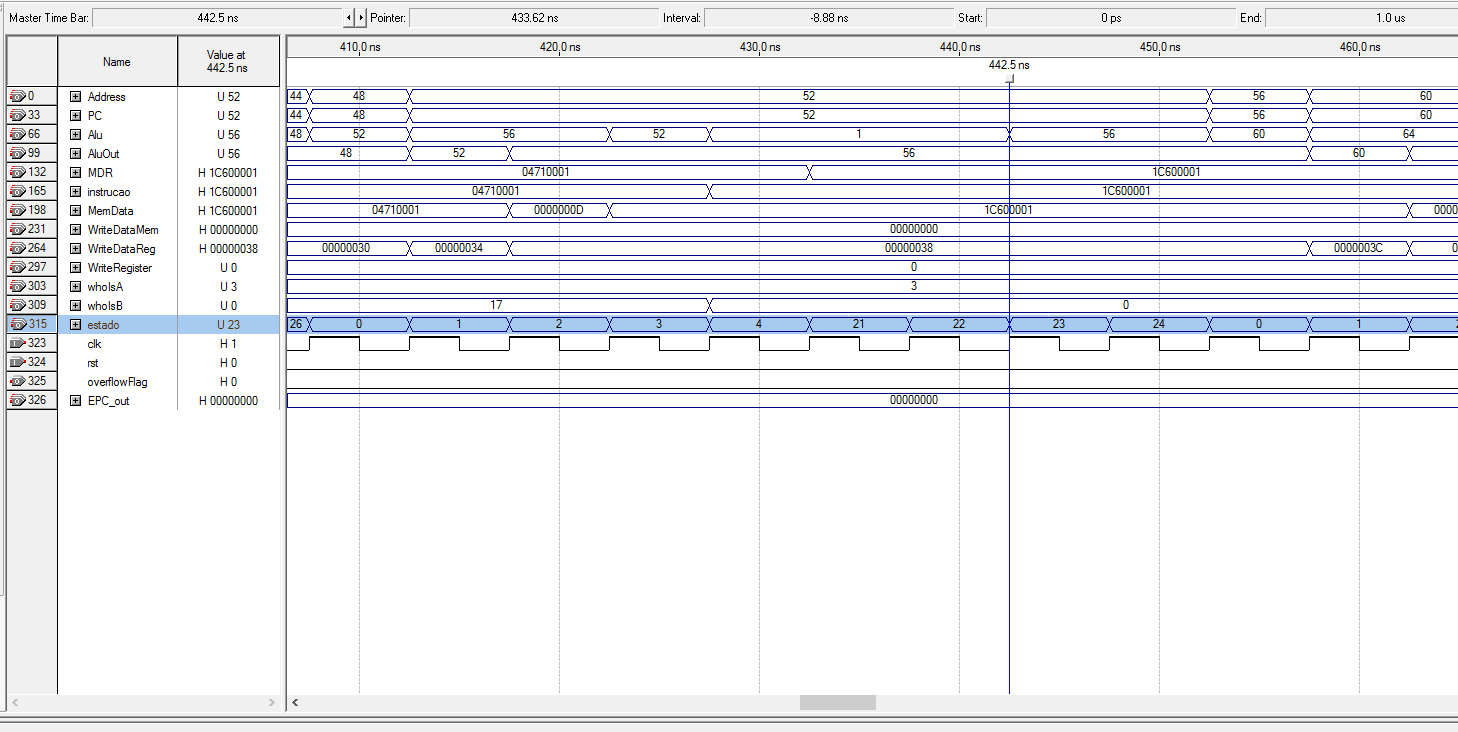
\includegraphics[scale=0.25]{bgtzsucesso.PNG}
    \end{center}
    
    \\
    \newpage
    \subsubsection{blez}
    {\it blez \$3, 5} falha;\\
    \begin{center}
        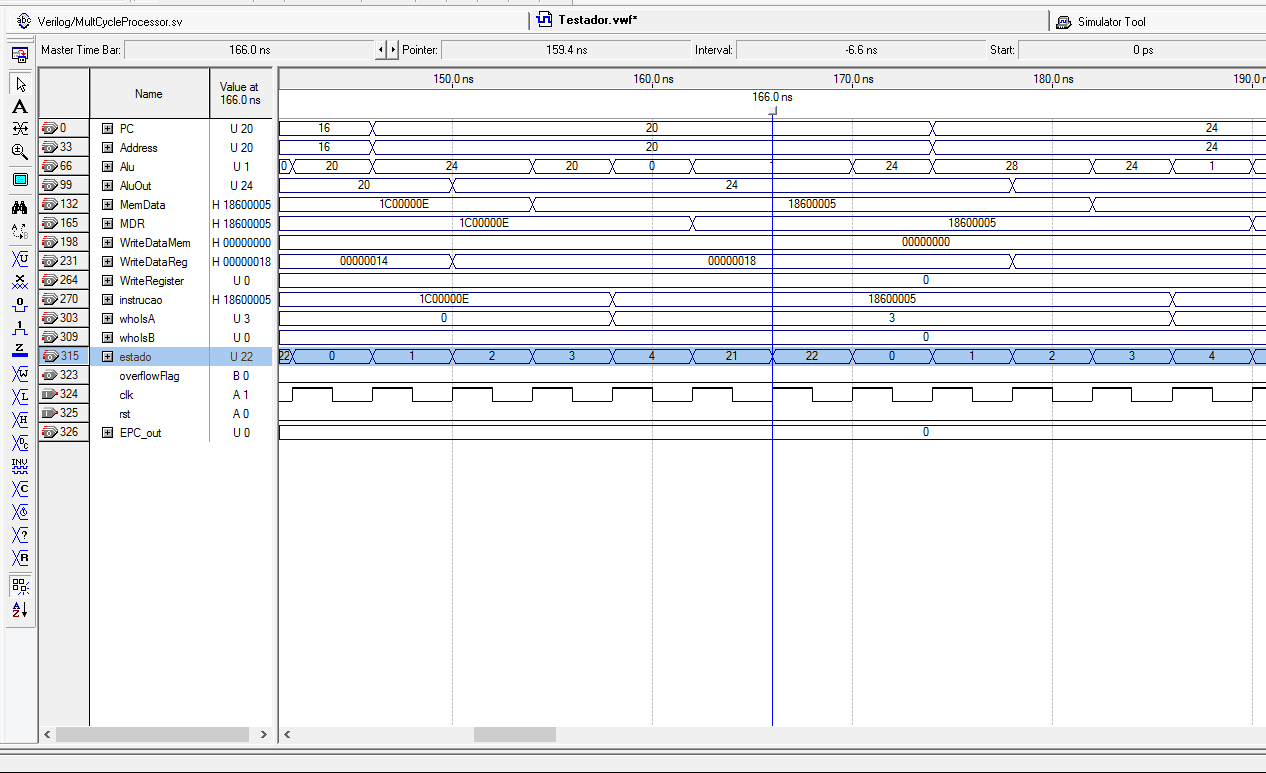
\includegraphics[scale=0.25]{blezfalha.PNG}
    \end{center}
    \\
    {\it blez \$0, 1} sucesso;\\
    \begin{center}
        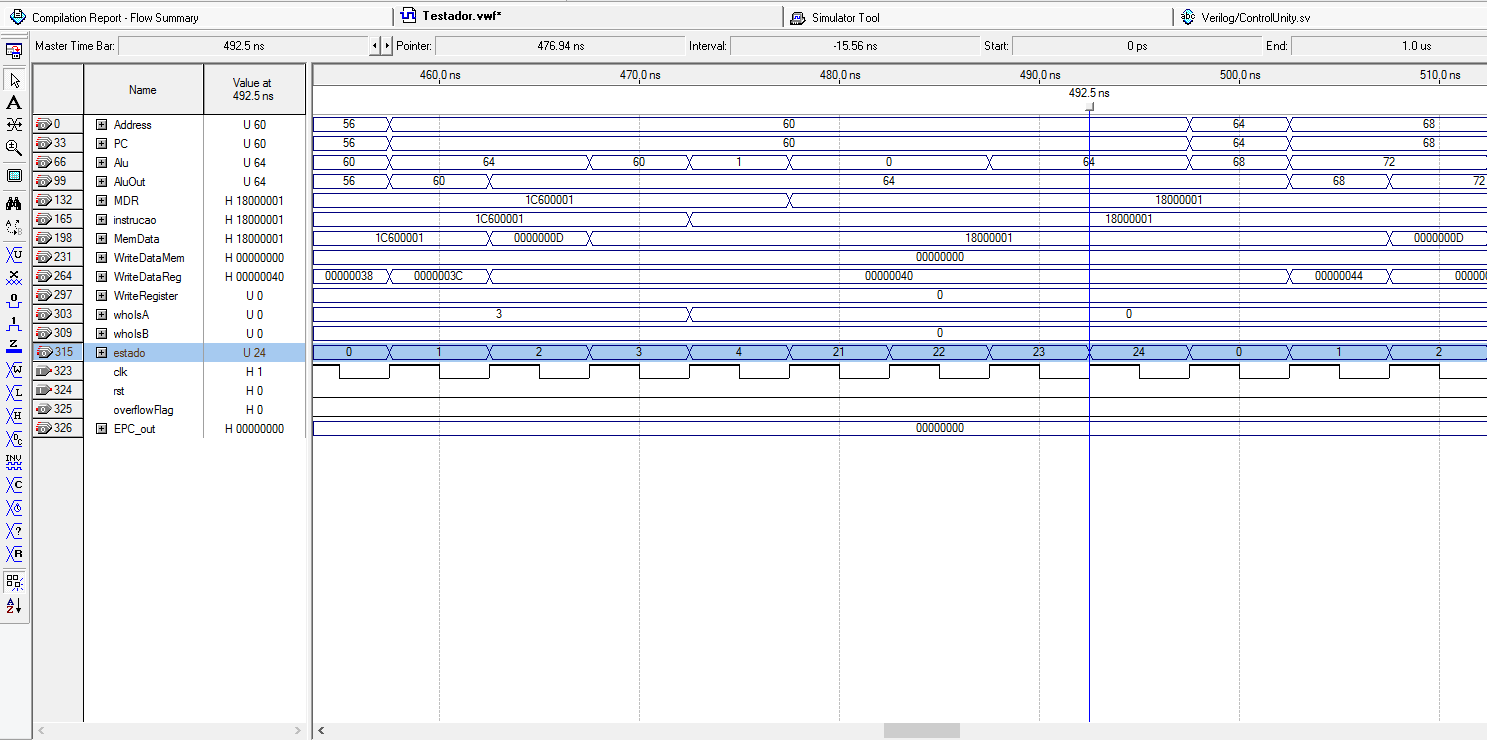
\includegraphics[scale=0.25]{blezsucesso.PNG}
    \end{center}
    
    \\
    \subsubsection{bltz}
    {\it bltz \$0, 8} falha;\\
    \begin{center}
        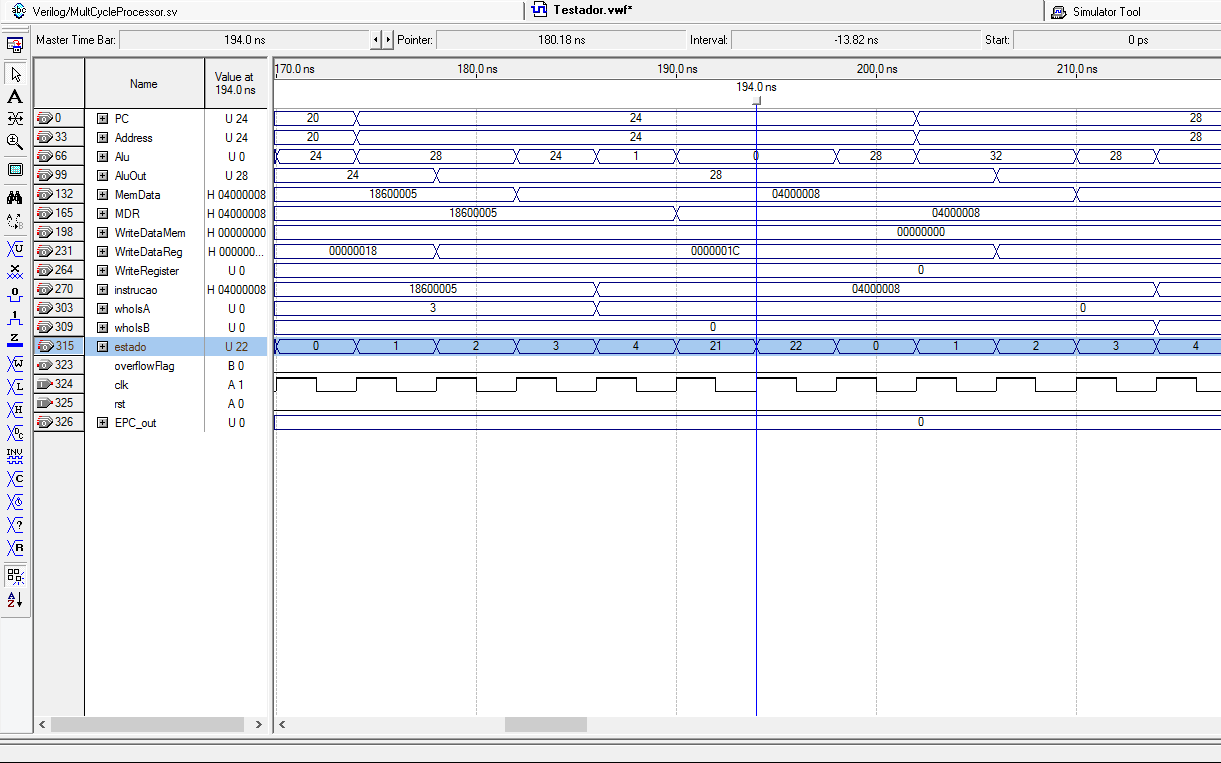
\includegraphics[scale=0.25]{bltzfalha.PNG}
    \end{center}
    \\
    \newpage
    {\it bltz \$2, 1} sucesso;\\
    \begin{center}
        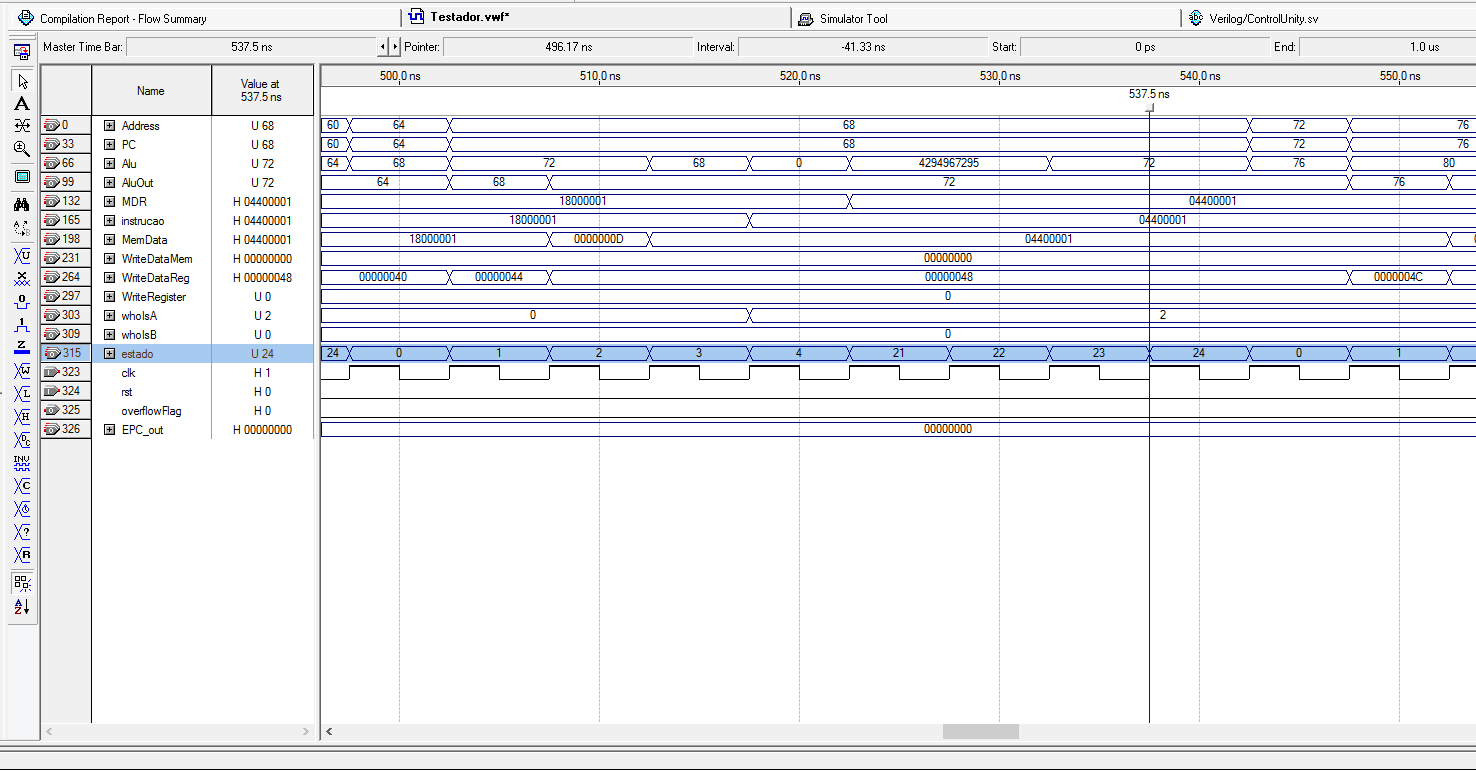
\includegraphics[scale=0.25]{bltzsucesso.PNG}
    \end{center}
    
    \\
    \subsubsection{bgezal}
    {\it bgezal \$2, 14} falha;\\
    \begin{center}
        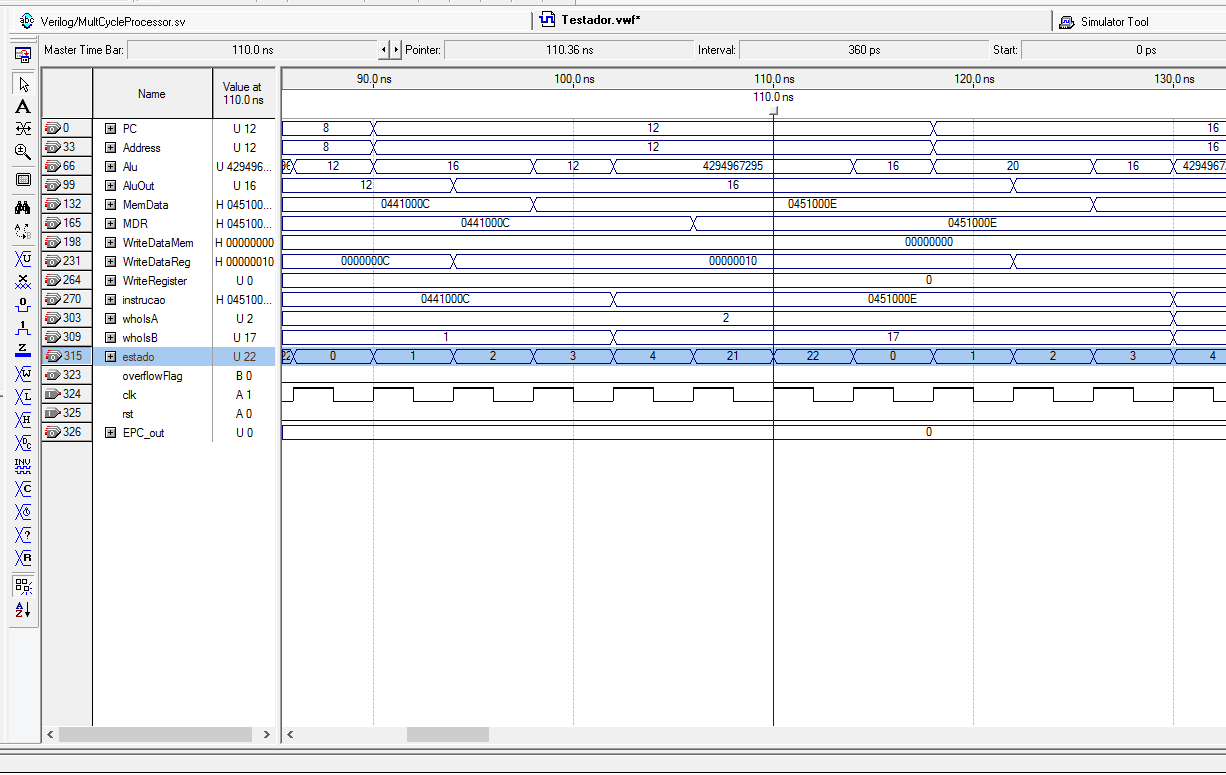
\includegraphics[scale=0.25]{bgezalfalha.PNG}
    \end{center}
    \\
    {\it bgezal \$3, 1} sucesso;\\
    \begin{center}
        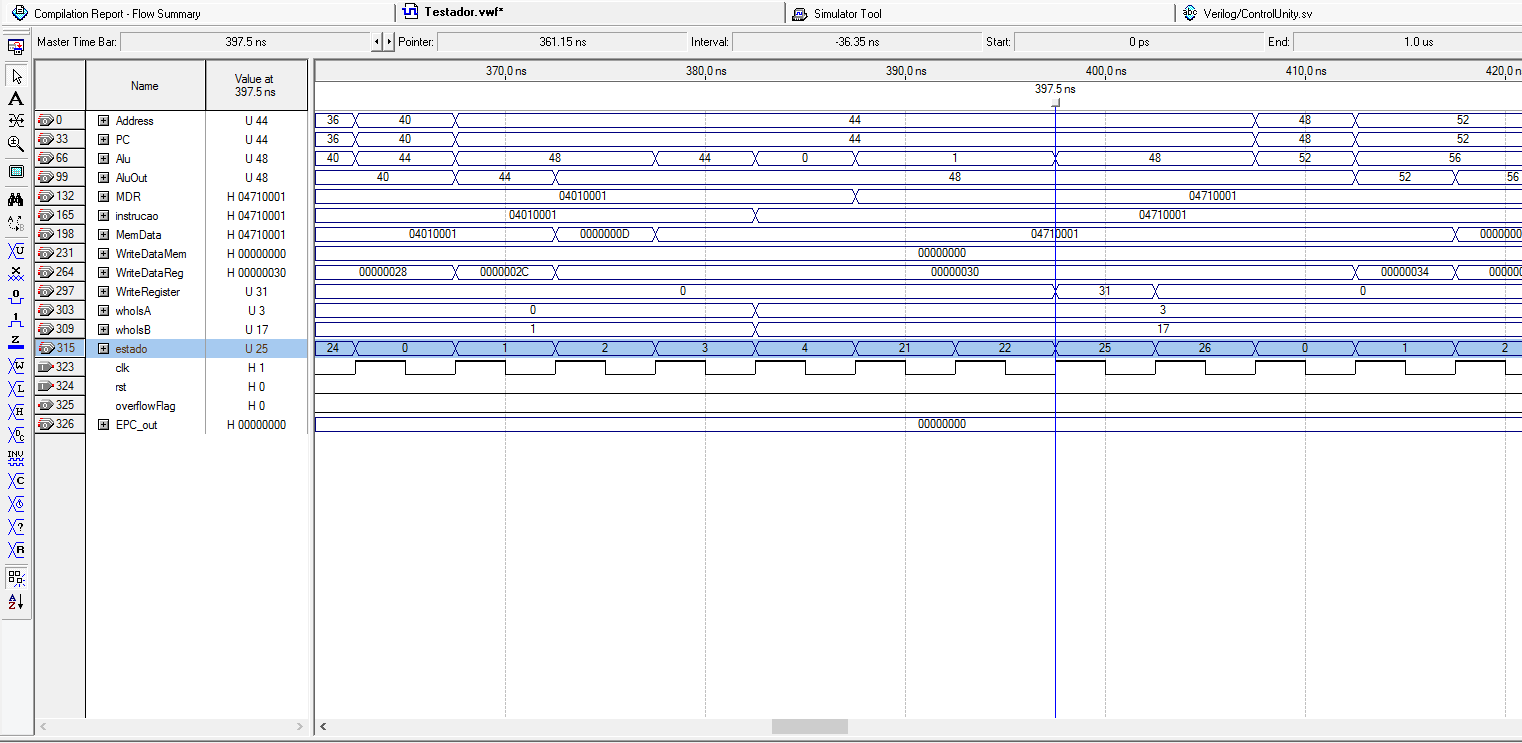
\includegraphics[scale=0.25]{bgezalsucesso.PNG}
    \end{center}
    
    \\
    \newpage
    \subsubsection{bltall}
    {\it bltall \$0, 5} falha;\\
    \begin{center}
        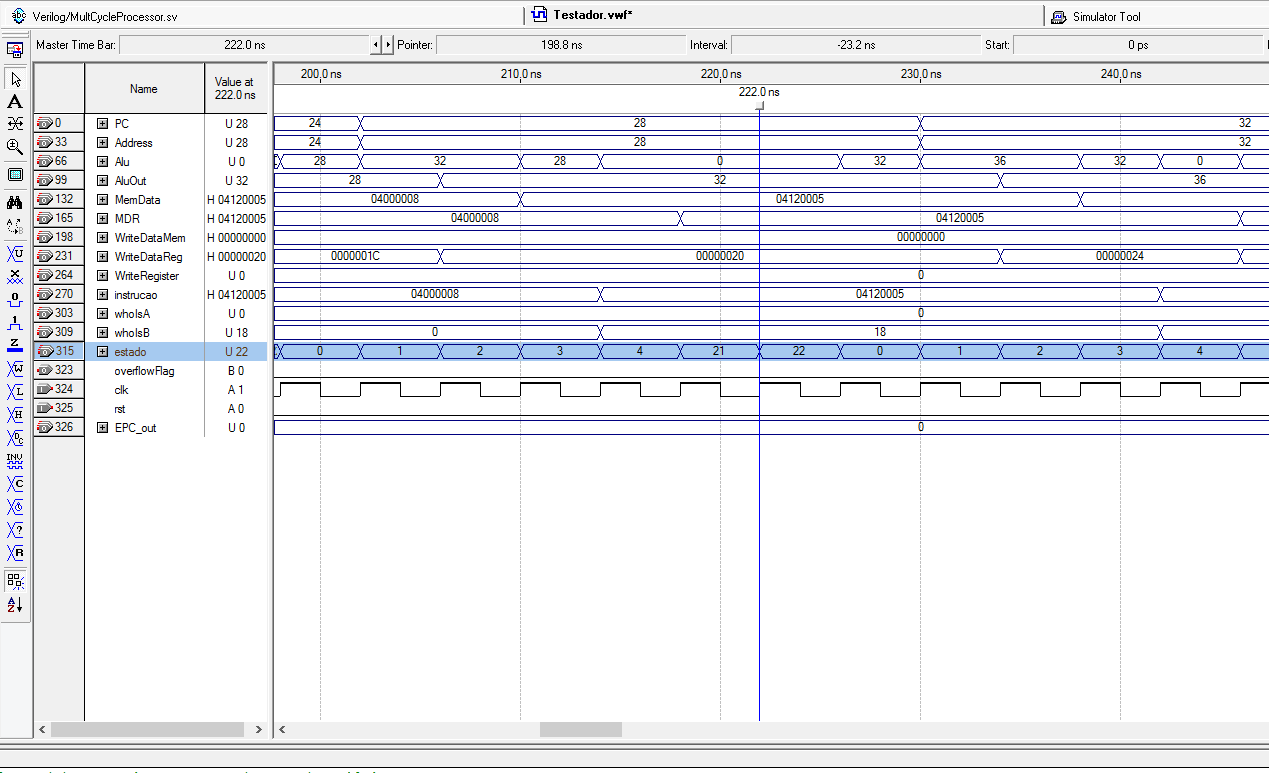
\includegraphics[scale=0.25]{bltallfalha.PNG}
    \end{center}
    \\
    {\it bltall \$2, 1} sucesso;\\
    \begin{center}
        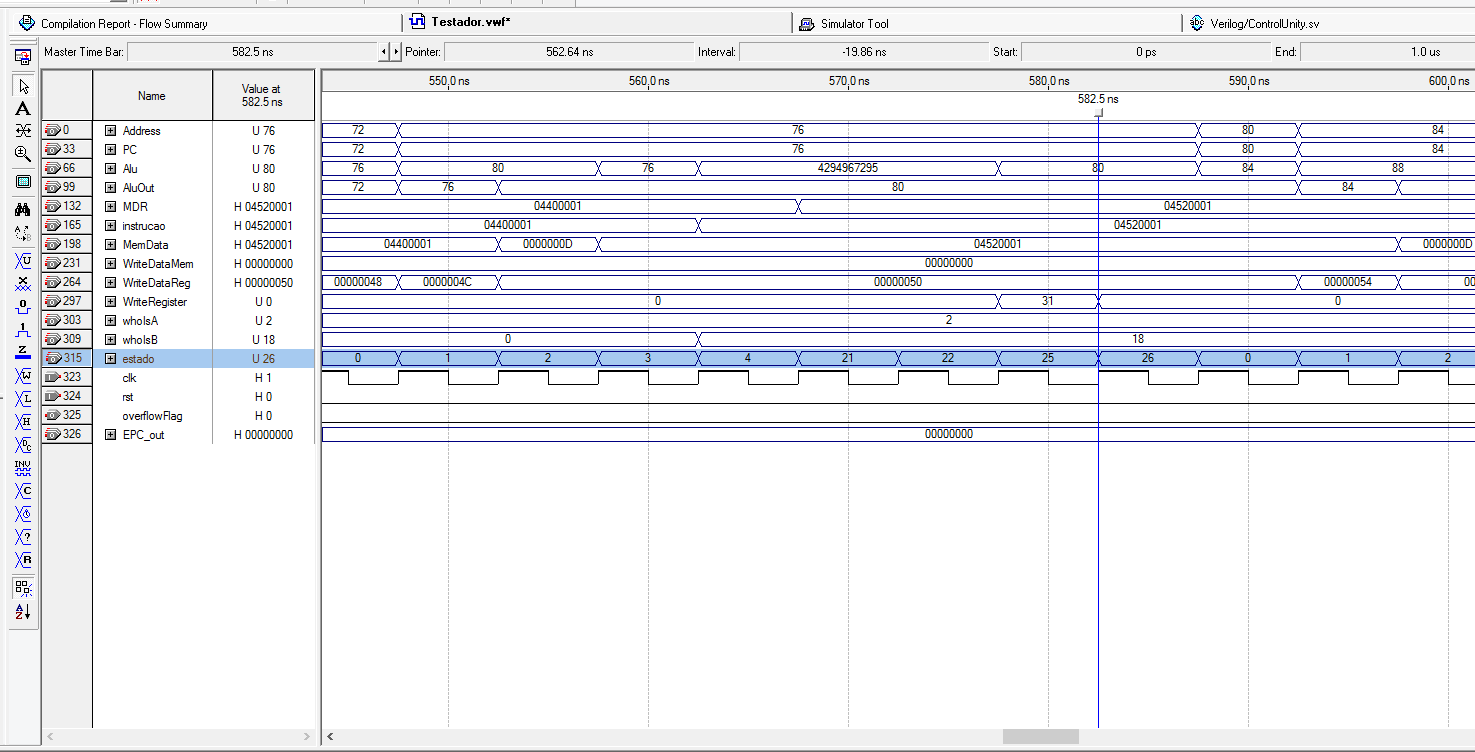
\includegraphics[scale=0.25]{bltallsucesso.PNG}
    \end{center}
    
    \\
    \subsubsection{lbu}
    {\it lbu \$5, 100(\$0)}
    \begin{center}
        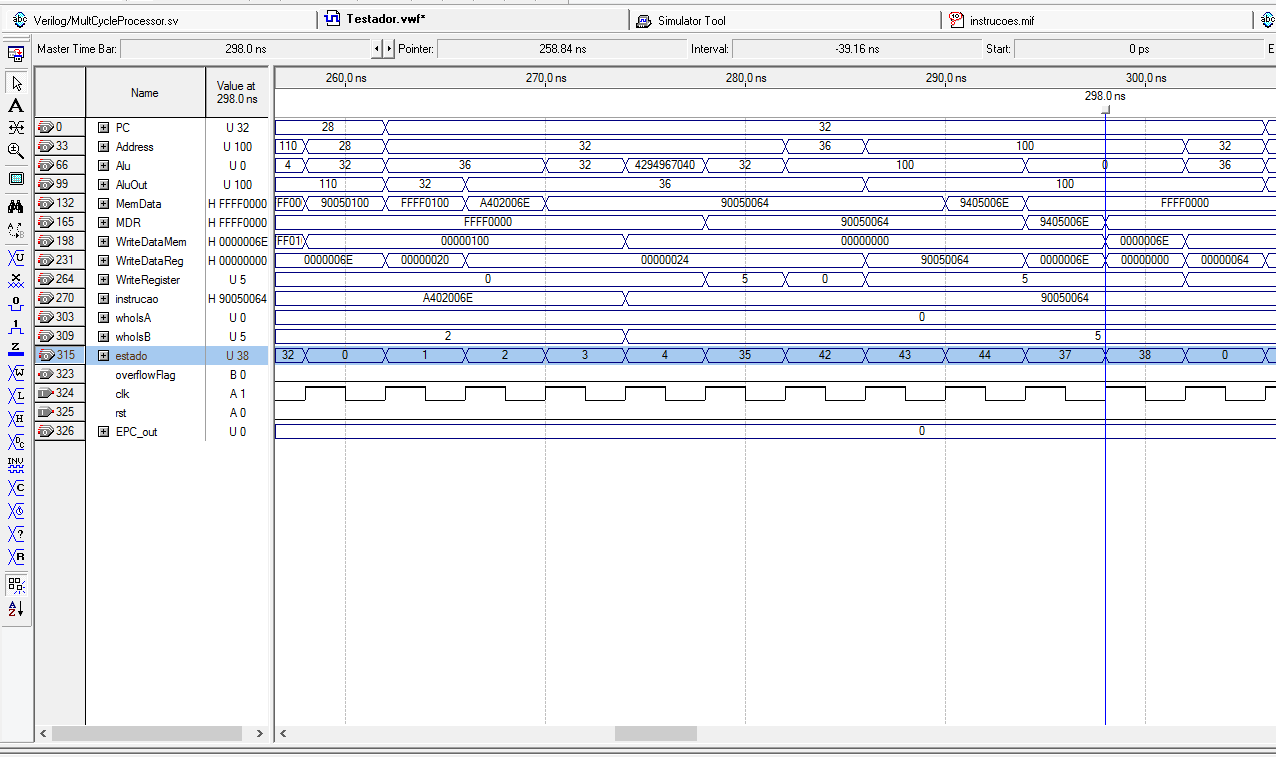
\includegraphics[scale=0.25]{lb.PNG}
    \end{center}
    
    \\
    \newpage
    \subsubsection{lhu}
    {\it lh \$5, 110(\$0)}
    \begin{center}
        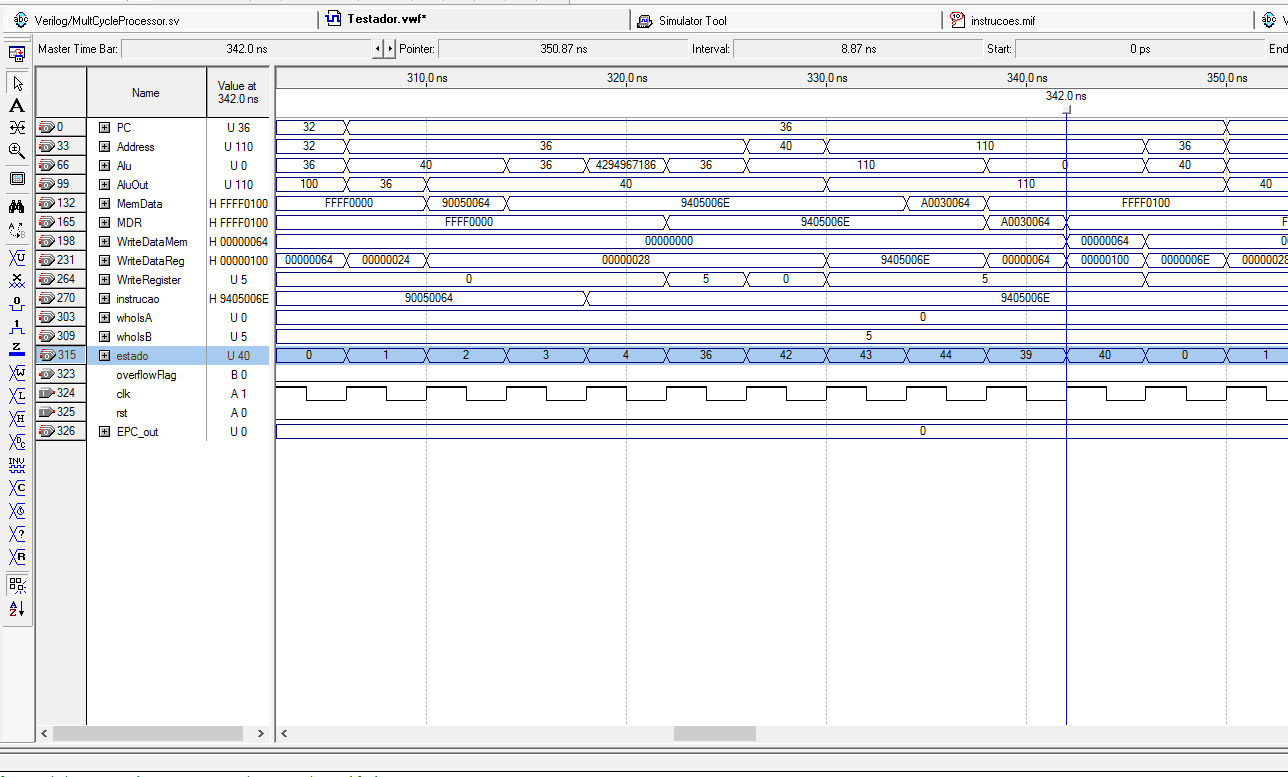
\includegraphics[scale=0.25]{lh.PNG}
    \end{center}
    
    \\
    \subsubsection{lui}
    {\it lui \$2, 1}\\
    \begin{center}
        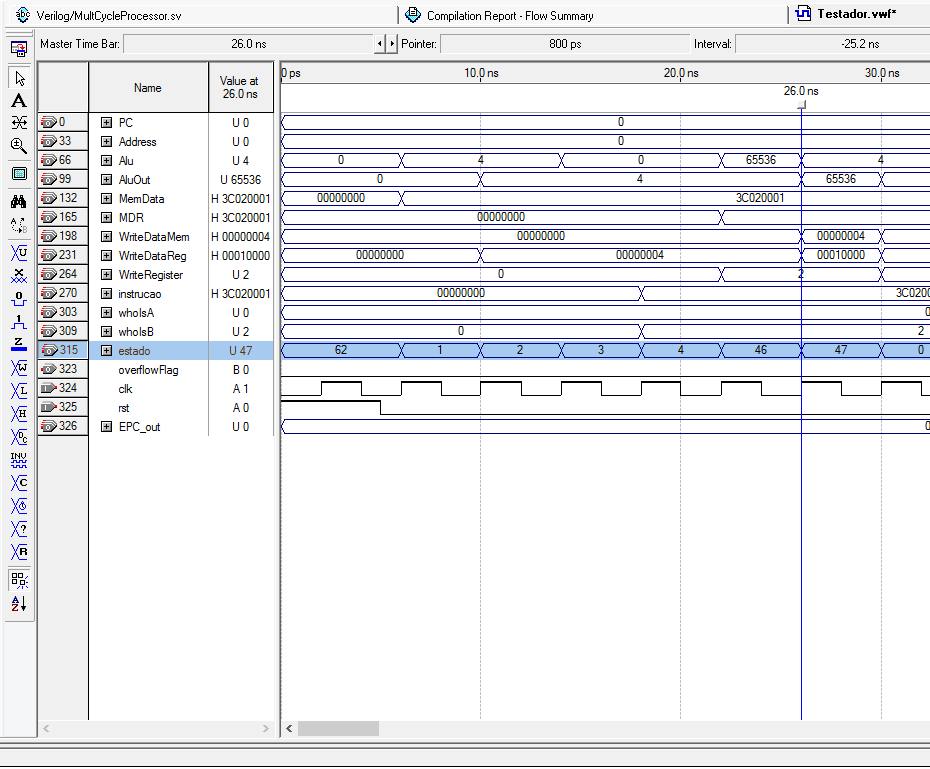
\includegraphics[scale=0.25]{lui.PNG}
    \end{center}
    
    \\
    \subsubsection{lw}
    {\it lw \$13, 180(\$0)}\\
    \begin{center}
        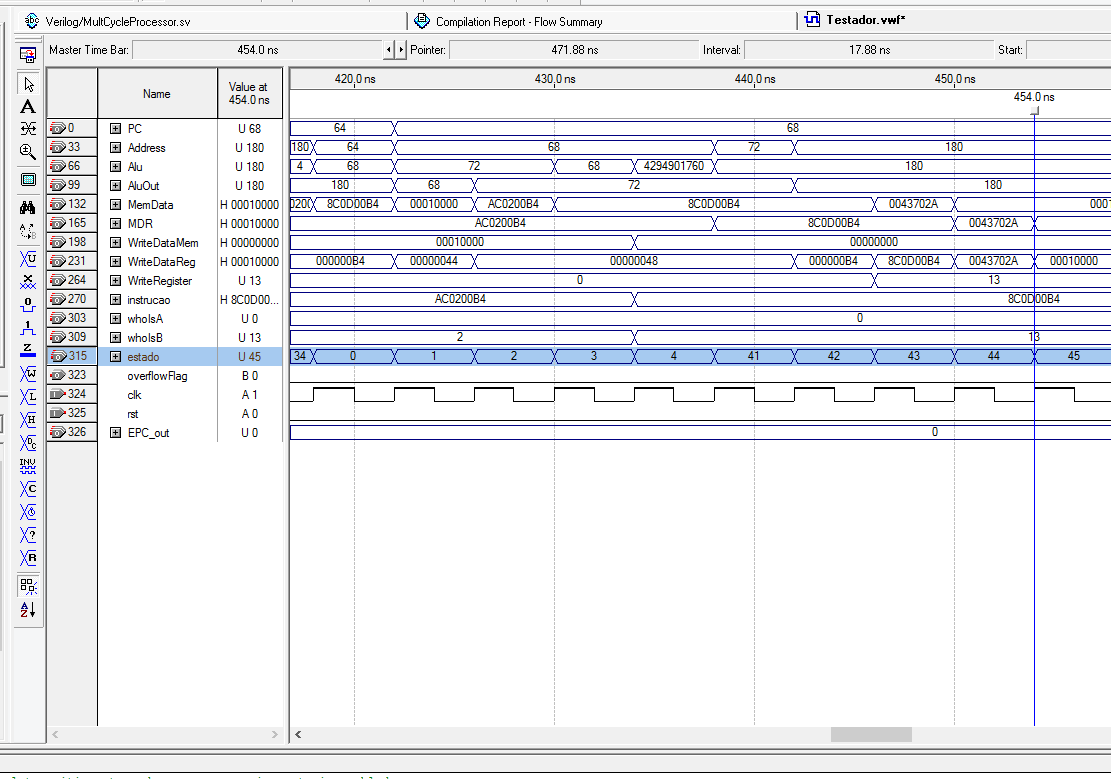
\includegraphics[scale=0.25]{lw.PNG}
    \end{center}
    
    \\
    \subsubsection{sb}
    {\it sb \$2, 100(\$0)}
    \begin{center}
        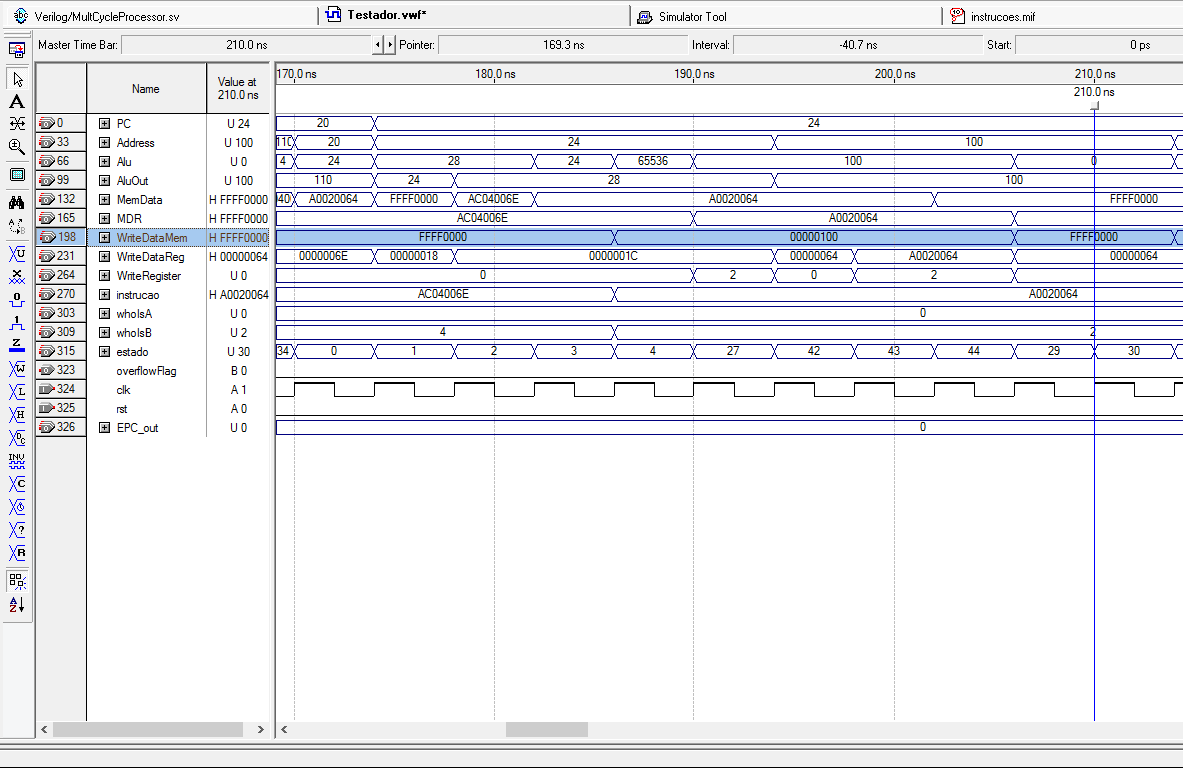
\includegraphics[scale=0.25]{sb.PNG}
    \end{center}
    
    \\
    \subsubsection{sh}
    {\it sh \$2, 110(\$0)}
    \begin{center}
        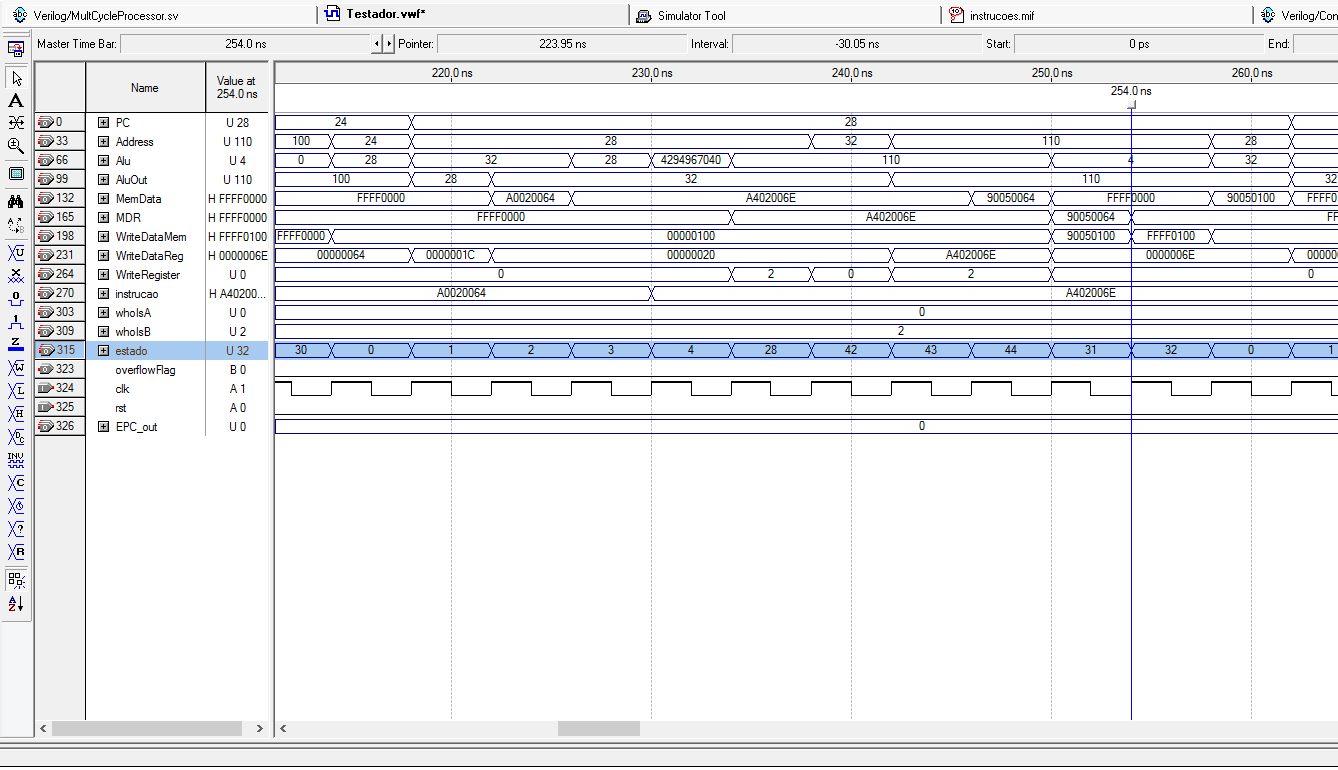
\includegraphics[scale=0.25]{sh.PNG}
    \end{center}
    
    \\
    \subsubsection{slti}
    {\it slti \$14, \$0, 0} falha;\\
    \begin{center}
        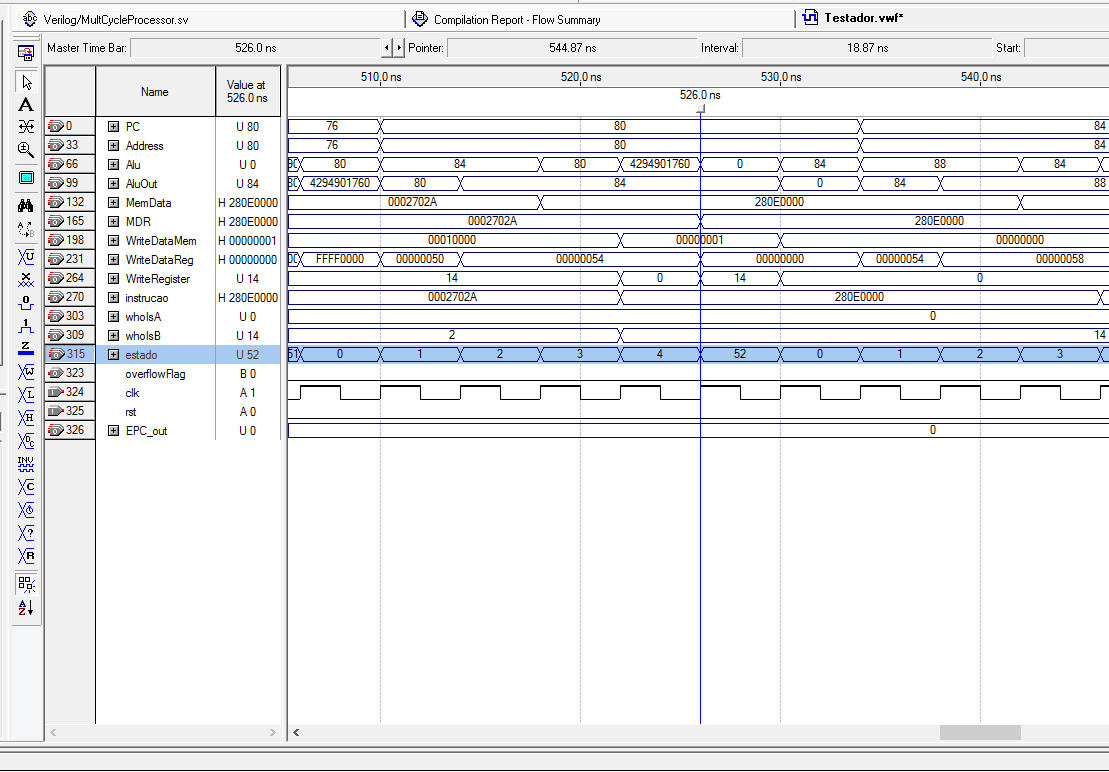
\includegraphics[scale=0.25]{sltifalha.PNG}
    \end{center}
    \\
    \newpage
    {\it slti \$14, \$0, 2} sucesso;\\
    \begin{center}
        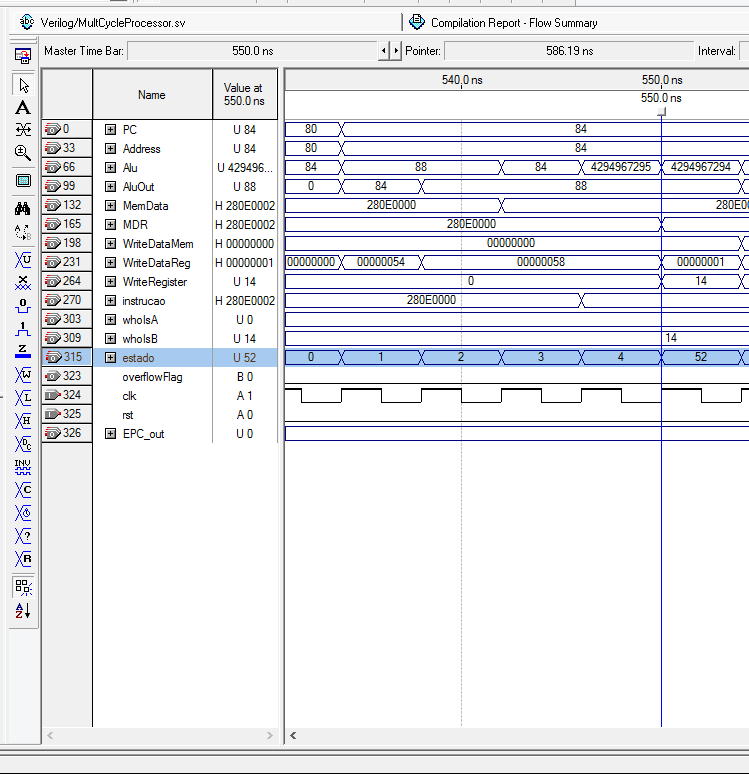
\includegraphics[scale=0.25]{sltisucesso.PNG}
    \end{center}
    
    \\
    \subsubsection{sw}
    {\it sw \$2, 180(\$0)}\\
    \begin{center}
        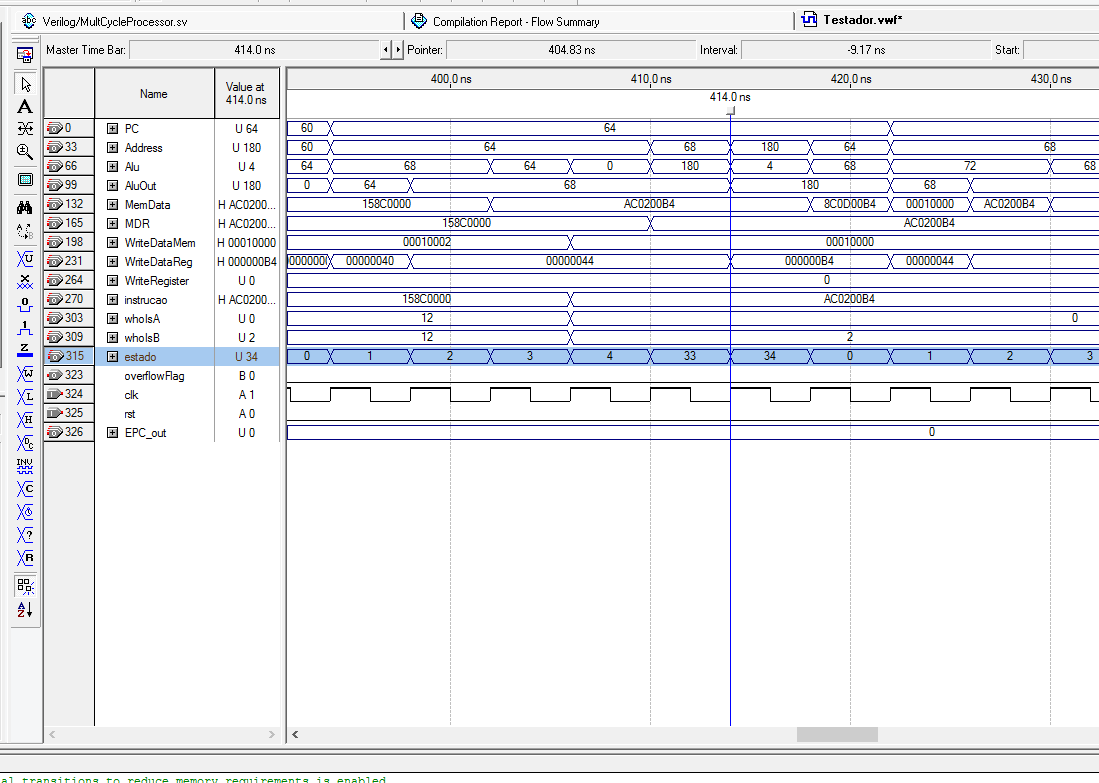
\includegraphics[scale=0.25]{sw.PNG}
    \end{center}
    
    \\
    \subsubsection{sxori}
    {\it xori \$12, \$2, 2}\\
    \begin{center}
        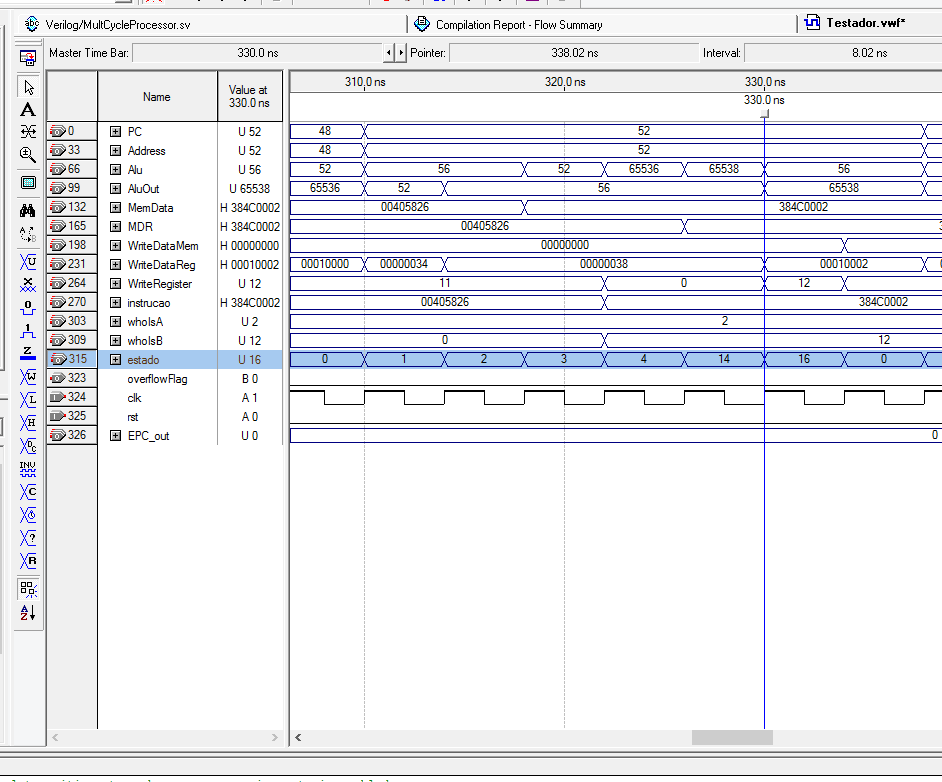
\includegraphics[scale=0.25]{xori.PNG}
    \end{center}
    
    \\
    \subsubsection{j} 
    {\it j 6}\\
    \begin{center}
        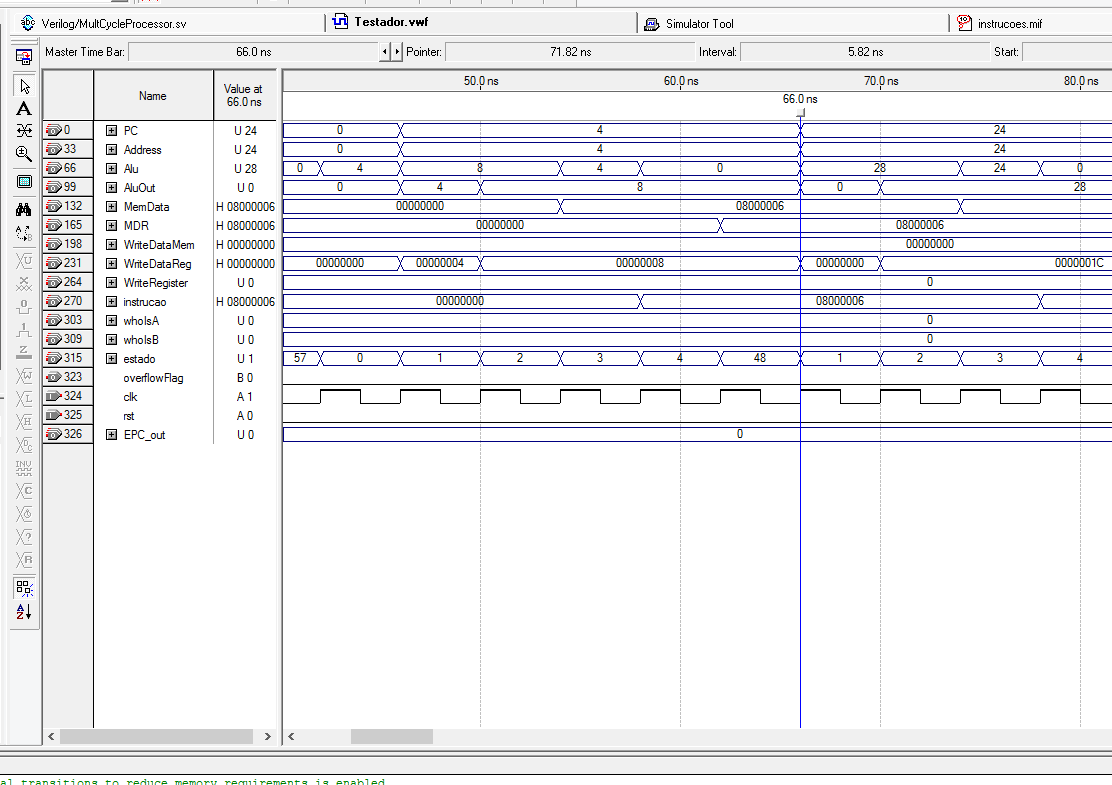
\includegraphics[scale=0.25]{j.PNG}
    \end{center}
    
    \\
    \subsubsection{rte} 
    {\it rte}\\
    \begin{center}
        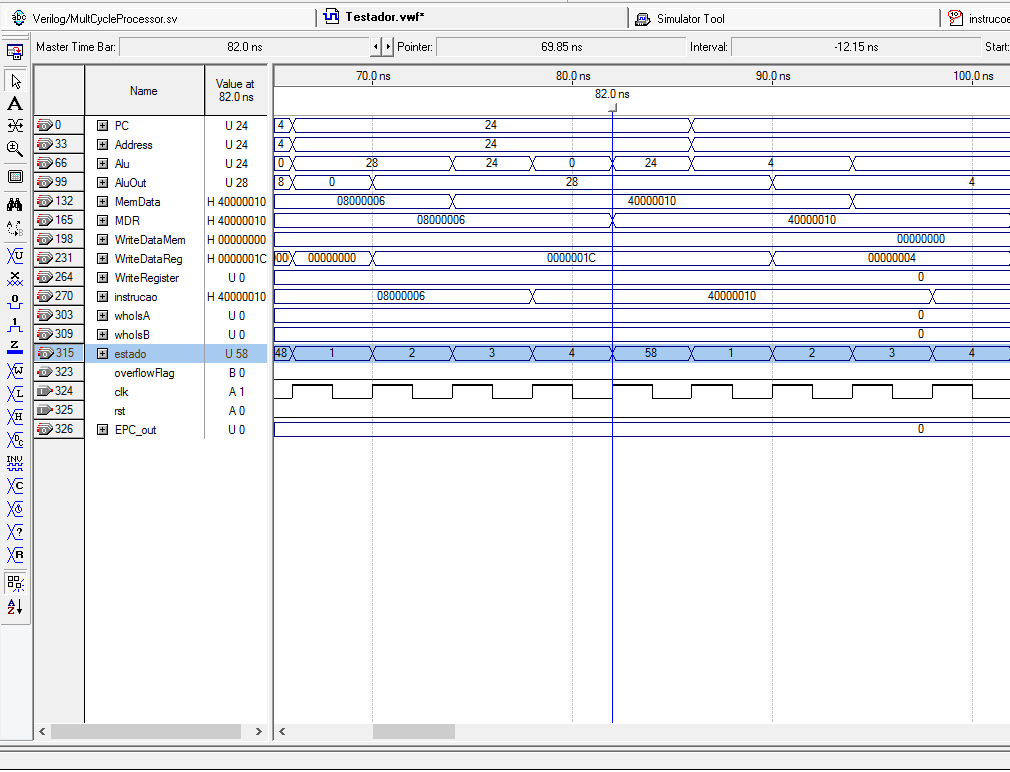
\includegraphics[scale=0.25]{rte.PNG}
    \end{center}
    
    \\
    \subsubsection{jal}
    {\it jal 4}\\
    \begin{center}
        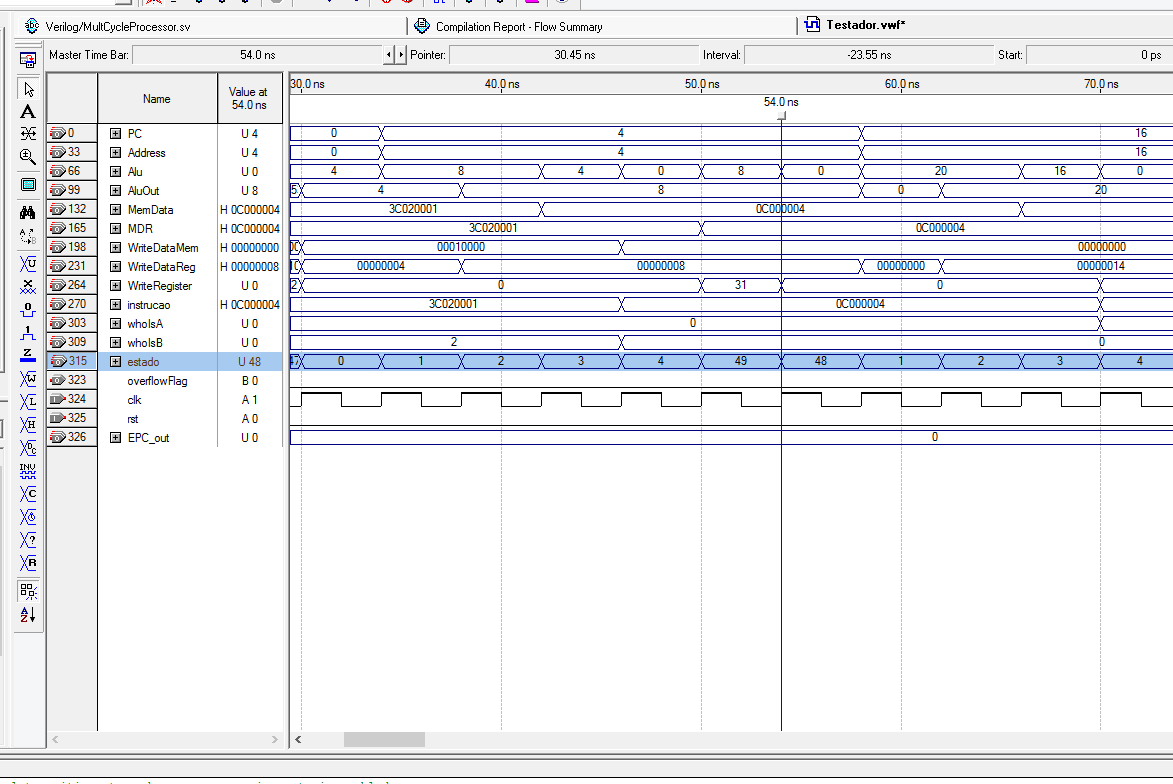
\includegraphics[scale=0.25]{jal.PNG}
    \end{center}
    
    \\
    \newpage
    \subsection{Módulos}
     \subsubsection{MultCycleProcessor}
    \textbf{Entradas}:
    \begin{enumerate}
        \item clk(1 bit): representa o clock do sistema.
        \item rst(1 bit): representa que, quando ativado, reinicia todo o sistema.\\
    \end{enumerate}
\\
    \textbf{Saídas}:
    \begin{enumerate}
        \item overflowFlag(1 bit): representa se o sinal de Overflow foi ativado.
        \item whoIsA(5 bits): representa qual registrador foi transferido pro RegA.
        \item whoIsB(5 bits): representa qual registrador foi transferido pro RegB.
        \item WriteRegister(5 bits): representa qual registrador vai ser possivelmente escrito.
        \item estado(7 bits): representa o estado no qual a Unidade de Controle se encontra.
        \item MemData(32 bits): representa o dado que está na saída do registrador de acesso a memória.
        \item WriteDataMem(32 bits): representa o dado que será possivelmente escrito na memória.
        \item WriteDataReg(32 bits): representa o dado que será possivelmente escrito em um registrador.
        \item MDR(32 bits): representa o dado que está na saída do registrador Memory Data Register.
        \item Alu(32 bits): representa o dado que está na saída da ULA.
        \item AluOut(32 bits): representa o dado que está na saída do registrador AluOut.
        \item PC(32 bits): representa o dado que está na saída do registrador PC (Program Counter).
        \item Address(32 bits): representa o endereço que vai ser lido/escrito na memória.
        \item instrucao(32 bits): representa a instrução que está saindo do Registrador de Instruções.
        \item EPC\_out(32 bits): representa o dado que está na saída do registrador EPC (Excepcion Program Counter).\\
    \end{enumerate}\\
    \begin{center}
        \includegraphics[scale=0.3]{MultCycleProcessor.PNG}
    \end{center}
    
    \newpage
    \subsubsection{ControlUnity}
    \textbf{Entradas}:
    \begin{enumerate}
         \item clk(1 bit): representa o clock do sistema.
         \item rst(1 bit): representa que, quando ativado, muda o estado para o estado {\it clean}.
         \item isTrue(1 bit): representa se o desvio de qualquer Branch será efetuado ou não.
         \item exceptReset(1 bit): representa se aconteceu alguma exceção ou não (overflow ou OpCode inválido).
         \item rt(5 bits): representa a parte da instrução referente ao {\it rt} (utilizado para distinguir os Branchs).
         \item OP(5 bits): representa o {\it OP Code} da função a ser executada.
         \item ari\_Func(5 bits): representa a parte {\it funct} do código binário da função, utilizado para distinguir as operações aritméticas.\\
    \end{enumerate}
\\
    \textbf{Saídas}:
    \begin{enumerate}
        \item PCWrite (1 bit): representa se o valor da entrada do registrador PC será passada para saída(1) ou não(0).
        \item IorD(1 bit): representa se o Address virá do registrador PC (0) ou do registrador AluOut(1).
        \item clear(1 bit): representa se o sistema será reiniciado(1) ou não(0).
        \item act\_regA(1 bit): representa se o valor da entrada do registrador regA será passada para saída(1) ou não(0).
        \item act\_regB(1 bit): representa se o valor da entrada do registrador regB será passada para saída(1) ou não(0).
        \item act\_ALUout(1 bit): representa se o valor da entrada do registrador AluOut será passada para saída(1) ou não(0).
        \item act\_memData(1 bit): representa se o valor da entrada do registrador MDR será passada para saída(1) ou não(0).
        \item signExtendSrc(1 bit): representa o seletor do multiplexador que define qual sign extend será utilizado na operação (o normal ou o referente ao Lui).
        \item savePCexcep(1 bit): representa se o valor da entrada do registrador EPC será passada para saída(1) ou não(0).
        \item MemWrite(1 bit): representa se o valor em WriteDataMemory será escrito(1) ou não(0) na memória.
        \item IRWrite(1 bit): representa se o valor na entrada do registrador de instruções será passado para as saídas(1) ou não(0).
        \item AluSrcA(1 bit): representa o seletor do multiplexador ligado à entrada A da Alu (0 = regA e 1 = PC).
        \item RegWrite(1 bit): representa se o valor em WriteDataReg será escrito(1) ou não(0) no registrador WriteRegister.
        \item act\_cleanA(1 bit): representa se o valor no registrador regA será zerado(1) ou não(0).
        \item act\_cleanB(1 bit): representa se o valor no registrador regB será zerado(1) ou não(0).
        \item act\_overflow(1 bit): representa se o sinal de {\it Overflow} da Alu será considerado(1) ou não(0).
        \item act\_ShiftOrSet(1 bit): representa o seletor do multiplexador que seleciona se o dado enviado para o multiplexador do WriteDataReg será o valor de um Shift(0) ou de um Set Less Than(1).
        \item AluSrcB(2 bits): representa o seletor do multiplexador ligado à entrada B da Alu (0 = regB, 1 = 4, 2 = signExtend, 3 = signExtend + shiftLeft2).
        \item RegDist(2 bits): representa o seletor do multiplexador que define qual será o registrador que será possivelmente escrito (0 = rs, 1 = rt, 3 = 31, 4 = 0).
        \item MemToReg(2 bits): representa o seletor do multiplexador que define qual dado será escrito no registrador (0 = AluOut, 1 = MDR, 2 = saída da Alu, 3 = set less).
        \item act\_MemoryDataWrite(2 bits): representa o seletor do multiplexador que define se o que será escrito na memória serão 32 bits (0), uma {\it half word}(1) ou um byte(2).
        \item writeDataRegSel(2 bits): representa o seletor do multiplexador que define se o que será escrito na memória serão 32 bits (0), uma {\it half word}(1), um byte(2) ou o resultado de um Shift/SetLess(3).
        \item ALUOp(3 bits): representa o seletor da função da Alu (tabela na especificação do projeto).
        \item PCSource(3 bits): representa o seletor do multiplexador que define a origem da entrada do registrador PC (0 = saída da Alu, 1 = AluOut, 2 = endereço de jump, 3 = regA, 4 = epc).
        \item estado(7 bits): representa o estado\footnote{checar a o tópico 4, página 21.} em que a unidade de controle se encontra.\\
    \end{enumerate}\\
    \begin{center}
        \includegraphics[scale=0.4]{ControlUnity.PNG}
    \end{center}
\\
    
    \newpage
    \subsubsection{mux4Memory}
    \textbf{Entradas}:
    \begin{enumerate}
        \item Seletor(1 bit): representa o seletor desse multiplexador (0 = entrada0, 1 = entrada1 + entrada3[31:16], 2 = entrada2 + entrada3[31:8], 3 = entrada3)
        \item entrada0(32 bits): representa a saída caso o seletor seja igual a 0.
        \item entrada1(16 bits): representa a {\it half word} da saída caso o seletor seja igual a 1.
        \item entrada2(8 bits): representa o byte da saída caso o seletor seja igual a 2..
        \item entrada3(32 bits): representa a saída caso o seletor seja igual a 3.\\
    \end{enumerate}
    \\
    \textbf{Saídas}:
    \begin{enumerate}
        \item saida(32 bits): representa a saída do multiplexador.\\
    \end{enumerate}\\
    \begin{center}
        \includegraphics[scale=0.4]{mux4Memory.PNG}
    \end{center}
    \\
    \newpage
    \subsubsection{mux4LoadB}
    \textbf{Entradas}:
    \begin{enumerate}
        \item Seletor(1 bit): representa o seletor desse multiplexador (0 = entrada0, 1 = entrada1 + 16'd0, \\2 = entrada2 + 24'd0, 3 = entrada3).
        \item entrada0(32 bits): representa a saída caso o seletor seja igual a 0.
        \item entrada1(16 bits): representa a {\it half word} da saída caso o seletor seja igual a 1.
        \item entrada2(8 bits): representa o byte da saída caso o seletor seja igual a 2..
        \item entrada3(32 bits): representa a saída caso o seletor seja igual a 3.\\
    \end{enumerate}
    \\
    \textbf{Saídas}:
    \begin{enumerate}
        \item saida(32 bits): representa a saída do multiplexador.\\
    \end{enumerate}\\
    \begin{center}
        \includegraphics[scale=0.4]{mux4LoadB.PNG}
    \end{center}
    
    \newpage
    \subsubsection{shiftleft2}
    \textbf{Entradas}:
    \begin{enumerate}
        \item entrada(32 bits): representa o dado a ser feito um shift left de 2 bits.\\
    \end{enumerate}
    \\
    \textbf{Saídas}:
    \begin{enumerate}
        \item saida(32 bits): representa o dado já feito um shift left de 2 bits.\\
    \end{enumerate}\\
    \begin{center}
        \includegraphics[scale=0.4]{shiftleft2.PNG}
    \end{center}
    \newpage
    \subsubsection{shiftRegOrImm}
    \textbf{Entradas}:
    \begin{enumerate}
        \item shamt(5 bits): representa a parte referente ao {\it shift amount} da operação.
        \item funct(6 bits): representa a parte referente à funcionalidade da operação.
        \item immediate(16 bits): representa a parte referente ao imediato da operação.\\
    \end{enumerate}
    \\
    \textbf{Saídas}:
    \begin{enumerate}
        \item saida(5 bits): representa a quantidade de shifts que será realizado pelo registrador de deslocamento.\\
    \end{enumerate}\\
    \begin{center}
        \includegraphics[scale=0.4]{shiftRegOrImm.PNG}
    \end{center}
    
    \newpage
    \subsubsection{InstrucJoin}
    \textbf{Entradas}:
    \begin{enumerate}
        \item instr\_2521(5 bits): representa do bit 25 ao bit 21 da instrução.
        \item instr\_2016(5 bits): representa do bit 20 ao bit 16 da instrução.
	    \item instr\_150(16 bits): representa do bit 16 ao bit 0 da instrução.\\
    \end{enumerate}
    \\
    \textbf{Saídas}:
    \begin{enumerate}
        \item instr\_250(32 bits): representa a junção do bit 25 ao bit 0 da instrução.\\
    \end{enumerate}\\
    \begin{center}
        \includegraphics[scale=0.4]{InstrucJoin.PNG}
    \end{center}
    \\
    \newpage
    \subsubsection{PCInstrucJoin}
    \textbf{Entradas}:
    \begin{enumerate}
        \item PC\_end(4 bits): representa os 4 bits mais significativos do registrador PC.
        \item sign\_extend\_instr(32 bits): representa a junção de todas as instruções.\\
    \end{enumerate}
    \\
    \textbf{Saídas}:
    \begin{enumerate}
        \item jmp\_address(32 bits): representa a junção dos 28 bits da instrução com 2 shifts left com os últimos 4 bits de pc.\\ 
    \end{enumerate}\\
    \begin{center}
        \includegraphics[scale=0.4]{PCInstrucJoin.PNG}
    \end{center}
    \\
    
    \newpage
    \subsubsection{SignExtendLui}
    \textbf{Entradas}:
    \begin{enumerate}
        \item extend(16 bits): representa o dado que será estendido de 16 para 32 bits.\\
    \end{enumerate}
    \\
    \textbf{Saídas}:
    \begin{enumerate}
        \item extended(32 bits): representa o dado estendido de 16 para 32 bits.\\
    \end{enumerate}\\
    \begin{center}
        \includegraphics[scale=0.4]{SignExtendLui.PNG}
    \end{center}
    \\
    \newpage
    \subsubsection{SignExtend}
    \textbf{Entradas}:
    \begin{enumerate}
         \item extend(16 bits): representa o dado que será estendido de 16 para 32 bits.\\
    \end{enumerate}
    \\
    \textbf{Saídas}:
    \begin{enumerate}
        \item extended(32 bits): representa o dado estendido de 16 para 32 bits.\\
    \end{enumerate}\\
    \begin{center}
        \includegraphics[scale=0.4]{SignExtend.PNG}
    \end{center}
    \\
    \newpage
    \subsubsection{setLessThanExtend}
    \textbf{Entradas}:
   \begin{enumerate}
        \item entrada(1 bit): representa o sinal de slt ou slti.\\
    \end{enumerate}
    \\
    \textbf{Saídas}:
    \begin{enumerate}
        \item saida(32 bits): representa o sinal de slt ou slti estendido para 32 bits.\\
    \end{enumerate}\\
    \begin{center}
        \includegraphics[scale=0.4]{setLessThanExtend.PNG}
    \end{center}

    
    \newpage
    \subsubsection{branchSelector}
    \textbf{Entradas}:
   \begin{enumerate}
        \item zeroFlag(1 bit): representa o sinal de zero da ALU.
        \item negativeFlag(1 bit): representa o sinal de negativo da ALU.
        \item clk(1 bit): representa o clock do sistema.
        \item rt (5 bits): representa a parte do código da operação referente ao {\it rt}.
        \item OPCode(6 bits): representa a parte do código da operação referente ao {\it OP Code}.\\
    \end{enumerate}
    \\
    \textbf{Saídas}:
    \begin{enumerate}
        \item saida(1 bit): representa se o desvio do branch será feito ou não.\\
    \end{enumerate}\\
    \begin{center}
        \includegraphics[scale=0.4]{branchSelector.PNG}
    \end{center}
    \\
    \newpage
    \subsubsection{shiftWise}
    \textbf{Entradas}:
   \begin{enumerate}
        \item clk(1 bit): representa o clock do sistema.
        \item funct(6 bits): representa a parte referente à funcionalidade da operação.\\
    \end{enumerate}
    \\
    \textbf{Saídas}:
    \begin{enumerate}
        \item shiftFunction(3 bits): representa qual operação será executado no registrador de deslocamento.\\
    \end{enumerate}\\
    \begin{center}
        \includegraphics[scale=0.4]{shiftWise.PNG}
    \end{center}
    
    \newpage
    \section{Observação}
    Os módulos mux8, mux4 e mux2 são multiplexadores de 8, 4 e 2 entradas, respectivamente, e com saídas de 32 bits e seus funcionamentos são triviais, assim como mux4RegBank, que é um multiplexador de 4 entradas e saída de 5 bits, então não foram descritos na sessão de \textbf{Descição dos módulos}\footnote{A partir da página 7.}.\\
    O Registrador de Deslocamento também foi alterado, pois ele só recebia quantidade de shifts de até 3 bits({\textless =7) e o Processador implementado pela equipe tem necessidade de receber até 5 bits(\textless =31) de quantidade de shifts.\\
    Após o desvio ser feito nas operações de {\it branch}, é feito uma soma de PC + 4 antes de analisar a instrução pois, nesta implementação, o endereço presente no registrador PC é o endereço da instrução que está sendo executada no momento e o desvio instruído pela especificação considera que o endereço presente em PC é o endereço da próxima instrução (PC + 4). Por isso, antes de executar a instrução, é feito um acréscimo em PC.
    
    \newpage
    \section{Conclusão}
    A equipe conclui, baseado nas simulações feitas no software {\it Quartus II 9.1sp2 Web Edition}, que é possível implementar, neste mesmo software, um Processador em Multiciclos, que executa as operações de {\it add, addu, and, jr, sll, sllv, slt, sra, srav, srl, sub, subu, xor, break, nop, rte, addi, addiu, andi, beq, bne, bgez, bgezal, bgtz, blez, bltz, bltall, lbu, lhu, lui, lw, sb, sh, slti, sw, sxori, j e jal}, totalizando 38 instruções, todas em Assembly MIPS.
    

\end{document}
